\documentclass[a4paper,12pt,english,twoside,openright]{memoir}
%\usepackage{etex} % probleme de reservation memoire pour les variables et certains packages.
%-------Packages--------------
\usepackage[T1]{fontenc}
\usepackage[utf8]{inputenc}
\usepackage{libertine}
\usepackage{fourier}%Symboles de separation
\usepackage{calc}
% \rmfamily
% \DeclareFontShape{T1}{lmr}{b}{sc}{<->ssub*cmr/bx/sc}{}
% \DeclareFontShape{T1}{lmr}{bx}{sc}{<->ssub*cmr/bx/sc}{}
% \font\curve=callig15 at 15pt
% \DeclareMathAlphabet{\mathpzc}{OT1}{pzc}{m}{it}% Definition des polices de caracteres speciales


%------------------ Mise en page ------------------
\usepackage{packages/MF-style_1}
\usepackage[some,top]{background}%marques de notes, faire un header pour style de page, ne pas depasser 1/4 hauteur de page au total
\SetBgContents{%
	\rule{.2cm}{.3cm}
}
\SetBgColor{black}
\usepackage{adjustbox}
%------------------ Graphics ------------------
\usepackage{wrapfig}
\usepackage{graphicx}

% \usepackage{graphicx,subfig}
% \usepackage{tikz}
\graphicspath{{Figures/}}
\usepackage{caption}
\captionsetup{textfont={small,it},format=plain,labelformat=empty,labelsep=none,justification=centerlast}


\usepackage{color}
\definecolor{gris1}{gray}{0.1}
\definecolor{gris2}{gray}{0.3}
\definecolor{gris3}{gray}{0.5}
\definecolor{gris4}{gray}{0.7}
\definecolor{gris5}{gray}{0.9}
\usepackage{packages/picins}

%%---------Langue---------
\usepackage[english]{babel}
\usepackage{makeidx}
\makeindex
%Avec \makeindex{nom} index des philosophes et index des citations
\usepackage{xspace}
\usepackage[protrusion=true,expansion=true,kerning, spacing]{microtype} %fine typo avec pdflatex, a règlé les erreures de boites horizontales canoniques
\usepackage{lipsum}

%-------Biblio version biblatex--------------
\usepackage[%
bibencoding=latin1,%
bibstyle=alphabetic,%
citestyle=alphabetic,%
sorting=nyt,%
language=english,%
isbn=false,%
doi=false,%
%eprint=true,%pour citation arxiv
%note=false,%
url=false
]{biblatex}
%\addbibresource{Galois.bib}%Pour nouvelles version de biblatex
\bibliography{Tesla}


\hypersetup{
	pdftitle = {My Inventions, Nikola Tesla's Autobiography},
	pdfauthor = {Nikola Tesla}
}

%%%%%%%%%%%%%%%%%%%%%%%%%%% Document %%%%%%%%%%%%%%%%%%%%%%%%%%%
\begin{document}
	\nocite{*}
	\frontmatter
%%------------------Title ------------------
\thispagestyle{empty}
% Original Title Template Peter Wilson	
{ 
\centering 
\vspace*{\baselineskip}

%Horizontal lines
\rule{\textwidth}{1.6pt}\vspace*{-\baselineskip}\vspace*{2pt} 
\rule{\textwidth}{0.4pt}\\[\baselineskip] 

\vspace*{1cm}
% Title
{\HUGE 	\bfseries
	MY INVENTIONS\\[\baselineskip] 
}

\vspace*{1cm}

%Horizontal lines
\rule{\textwidth}{0.4pt}\vspace*{-\baselineskip}\vspace{3.2pt} 
\rule{\textwidth}{1.6pt}\\[\baselineskip] 

\vspace*{.2cm}

\scshape 
% Tagline(s) or further description
{\Large
	By\\ \textsc{Nikola Tesla} \\
} 
\vspace*{1cm}

With\\ Original Illustrations\\ and\\ 
Forewords of H. Gernsback\\[\baselineskip]


\vspace*{4\baselineskip}

% Editor list
\emph{Edited by} \\
{\large Etaoin Shrdluc\par} 


\vfill % Whitespace between editor names and publisher logo


{\scshape 2014} \\[0.3\baselineskip] % Year published
{\large THE PUBLISHER}\par % Publisher
\vspace{1.5cm}
}

	\newpage
%%------------------Copyright ------------------	
	\thispagestyle{empty}
	{\vspace*{\stretch{1}}
	\centering\normalsize
	
	
\includegraphics[width=1cm]{cc-large.png}\hspace{1em}
	
\includegraphics[width=1cm]{by-large.png}\hspace{1em}
	
\includegraphics[width=1cm]{nc-large.png}\hspace{1em}
	
\includegraphics[width=1cm]{sa-large.png}
	
	\bigskip
	
	This work is licensed under the Creative Commons Attribution-NonCommercial-ShareAlike 4.0 International License, 2014. \\
	To view a copy of this license, visit \url{http://creativecommons.org/licenses/by-nc-sa/4.0/deed.en_US}.
	
	\bigskip
	
	{\small First published in the \textsc{Electrical Experimenter} magazine 1919.} 
	\par	
	}
	

\newpage
\clearforchapter	

\tableofcontents*
\newpage
\clearforchapter	

%%------------------Editor Preface ------------------
\thispagestyle{empty}
\markboth{Editor's Preface}{}
\markright{}
\vspace*{5em}
\begin{center}
	\bfseries
	\noindent {\Large\decofourleft~\textsc{I}~\decofourright}\\
	\noindent\rule{.5\linewidth}{1pt}\\
	\medskip
	{\noindent\LARGE Editor's Preface}
		\par
	
	\vspace*{5em}
\end{center}
\addcontentsline{toc}{section}{Editor's Preface}

{
%	History of document. 
	\emph{My Inventions} originally appeared in six series of the magazine \textsc{Electronical Experimenter} in 1919, written by Nikola Tesla when he was 63 years old. It has then been compiled, edited and extended with a 20 pages wonderful introduction and an \emph{Appendix: Hydrolic Analog of Tesla Two Phase Induction Motor} by Ben \textsc{Johnston} under the title \emph{My Inventions: The Autobiography of Nikola Tesla} in 1982. Note that the original six-part series published in Electrical Experimenter Magazine in 1919 has been republished in book form as: \emph{My Inventions, The Autobiography of Nikola Tesla (Hart Brothers, Williston, 1983)}.
	
	\medskip
	
	The first online version of Nikola Tesla's Autobiography was transcribed by John Roland Penner in 1994 from a small typed booklet, a photocopied and stapled version of \emph{The Strange Life of Nikola Tesla (Kolmogorov-Smirnov Publishing)}\footnote{Source: \url{http://en.wikipedia.org/wiki/My_inventions}, 23 June 2013.}.
			
	\medskip
		
	This text is an extended and edited version of the nearly unabridged electronic text available by \emph{Twenty-First Century Books}\footnote{See: \url{http://www.tfcbooks.com/special/my_inventions_index.htm}.}, which can be freely distributed and modified. It has been enhanced with the 16 original illustrations --with legends-- of the \textsc{Electronical Experimenter} edition\footnote{Collection at: \url{http://electricalexperimenter.com/}.}, as well as the 6 forewords signed by the quondam Editor H. \textsc{Gernsback}.
		
	\hfill -- \textsc{E. Shrdluc}.
		
	\newpage
	
	%Customize Bibliography
	\defbibheading{bibliography}[References]{%
	\subsection*{#1}%
	\markboth{#1}{#1}}
	\renewcommand*{\bibfont}{\small}
	\printbibliography[heading=bibliography]
	}

\mainmatter

%%------------------Chapitre 1 ------------------
	\thispagestyle{empty}
	\markboth{My Early Life}{}
	\markright{}
	\vspace*{5em}
	\begin{center}
		\bfseries
		\noindent {\Large\decofourleft~\textsc{I}~\decofourright}\\
		\noindent\rule{.5\linewidth}{1pt}\\
		\medskip
		{\noindent\LARGE My Early Life}
		
		\bigskip
		
		{\normalfont\smallskip\small\protect\parbox{.75\linewidth}{\itshape
				\lettrine[lines=2]{H}{ow} does the world's greatest inventor invent ? How does he carry out an invention? What sort of mentality has Nikola Tesla? Was his early life as commonplace as most of ours? What was the early training of one of the World's Chosen? These, and many other very interesting questions are answered in an incomparable manner by Nikola Tesla himself in this, his first article.
				
				In his autobiography, treating mainly on his early youth, we obtain a good insight into the wonderful life this man has led. It reads like a fairy tale, which has the advantage of being true. For Tesla is no common mortal. He has led a charmed life--struck down by the pest, the cholera and what not--given up by doctors at least three times as dead--we find him at sixty, younger than ever. You have never read the like before.\\
				
				\hfill --\scshape{Editor}.
			}
			\par
		}
		\vspace*{5em}

	\end{center}
	\addcontentsline{toc}{section}{My Early Life}
	
	
	\lettrine[lines=3]{T}{he} progressive development of man is vitally dependent on invention.  It is the most important 
	product of his creative brain.  Its ultimate purpose is the complete mastery of mind over the 
	material world, the harnessing of the forces of nature to human needs.  This is the difficult task of 
	the inventor who is often misunderstood and unrewarded.  But he finds ample compensation in 
	the pleasing exercises of his powers and in the knowledge of being one of that exceptionally 
	privileged class without whom the race would have long ago perished in the bitter struggle 
	against pitiless elements.  
	
	Speaking for myself, I have already had more than my full measure of this exquisite enjoyment, 
	so much that for many years my life was little short of continuous rapture.  I am credited with 
	being one of the hardest workers and perhaps I am, if thought is the equivalent of labor, for I have 
	devoted to it almost all of my waking hours.  But if work is interpreted to be a definite performance 
	in a specified time according to a rigid rule, then I may be the worst of idlers.  Every effort under 
	compulsion demands a sacrifice of life-energy.  I never paid such a price.  On the contrary, I have 
	thrived on my thoughts.  
	
	In attempting to give a connected and faithful account of my activities in this series of articles 
	which will be presented with the assistance of the Editors of the \textsc{Electrical Experimenter}
	and are chiefly addrest to our young men readers, I must dwell, however reluctantly, on the 
	impressions of my youth and the circumstances and events which have been instrumental in 
	determining my career.  

	
	Our first endeavors are purely instinctive, promptings of an imagination vivid and undisciplined.  
	As we grow older reason asserts itself and we become more and more systematic and designing.  
	But those early impulses, tho not immediately productive, are of the greatest moment and may 
	shape our very destinies.  Indeed, I feel now that had I understood and cultivated instead of 
	suppressing them, I would have added substantial value to my bequest to the world.  But not until 
	I had attained manhood did I realize that I was an inventor.  
	
	This was due to a number of causes.  In the first place I had a brother who was gifted to an 
	extraordinary degree—one of those rare phenomena of mentality which biological investigation 
	has failed to explain.  His premature death left my parents disconsolate.  We owned a horse 
	which had been presented to us by a dear friend.  It was a magnificent animal of Arabian breed, 
	possest of almost human intelligence, and was cared for and petted by the whole family, having 
	on one occasion saved my father's life under remarkable circumstances.  My father had been 
	called one winter night to perform an urgent duty and while crossing the mountains, infested by 
	wolves, the horse became frightened and ran away, throwing him violently to the ground.  It 
	arrived home bleeding and exhausted, but after the alarm was sounded immediately dashed off 
	again, returning to the spot, and before the searching party were far on the way they were met by 
	my father, who had recovered consciousness and remounted, not realizing that he had been lying 
	in the snow for several hours.  This horse was responsible for my brother's injuries from which he 
	died.  I witnest the tragic scene and altho fifty-six years have elapsed since, my visual impression 
	of it has lost none of its force.  The recollection of his attainments made every effort of mine seem 
	dull in comparison.  
	
	
	Anything I did that was creditable merely caused my parents to feel their loss more keenly.  So I 
	grew up with little confidence in myself.  But I was far from being considered a stupid boy, if I am 
	to judge from an incident of which I have still a strong remembrance.  One day the Aldermen 
	were passing thru a street where I was at play with other boys.  The oldest of these venerable 
	gentlemen—a wealthy citizen—paused to give a silver piece to each of us.  Coming to me he 
	suddenly stopt and commanded, "Look in my eyes." I met his gaze, my hand outstretched to 
	receive the much valued coin, when, to my dismay, he said, "No, not much, you can get nothing 
	from me, you are too smart." They used to tell a funny story about me.  I had two old aunts with 
	wrinkled faces, one of them having two teeth protruding like the tusks of an elephant which she 
	buried in my cheek every time she kist me.  Nothing would scare me more than the prospect of 
	being hugged by these as affectionate as unattractive relatives.  It happened that while being 
	carried in my mother's arms they asked me who was the prettier of the two.  After examining their 
	faces intently, I answered thoughtfully, pointing to one of them, "This here is not as ugly as the 
	other." 
	
	\begin{wrapfigure}{r}{0.65\textwidth}
		\vspace{-20pt}
		\begin{center}
			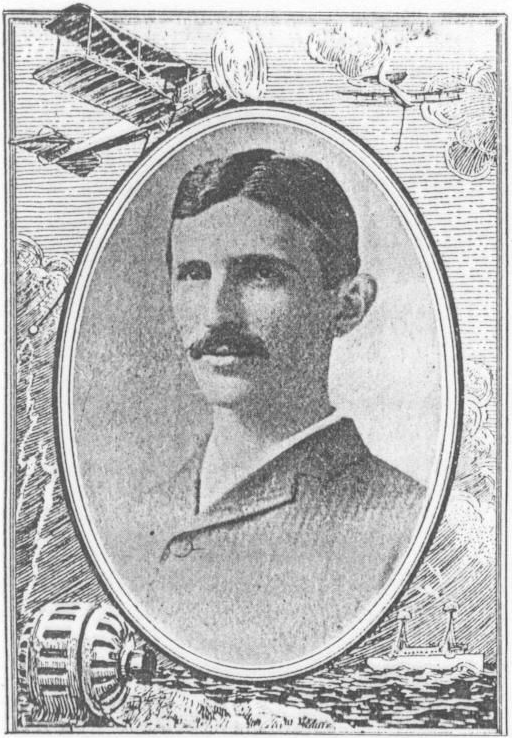
\includegraphics[width=0.63\textwidth]{Tesla-29.png}
		\end{center}
		\legend{Mr. Tesla at the Age of 29.}
		\vspace{-20pt}
	\end{wrapfigure}
	
	Then again, I was intended from my very birth for the clerical profession and this thought 
	constantly opprest me.  I longed to be an engineer but my father was inflexible.  He was the son 
	of an officer who served in the army of the Great Napoleon and, in common with his brother, 
	professor of mathematics in a prominent institution, had received a military education but, 
	singularly enough, later embraced the clergy in which vocation he achieved eminence.  He was a 
	very erudite man, a veritable natural philosopher, poet and writer and his sermons were said to 
	be as eloquent as those of Abraham a Sancta-Clara.  He had a prodigious memory and 
	frequently recited at length from works in several languages.  He often remarked playfully that if 
	some of the classics were lost he could restore them.  His style of writing was much admired.  He 
	penned sentences short and terse and was full of wit and satire.  The humorous remarks he 
	made were always peculiar and characteristic.  Just to illustrate, I may mention one or two 
	instances.  Among the help there was a cross-eyed man called Mane, employed to do work 
	around the farm.  He was chopping wood one day.  As he swung the axe my father, who stood 
	nearby and felt very uncomfortable, cautioned him, "For God's sake, Mane, do not strike at what 
	you are looking but at what you intend to hit." On another occasion he was taking out for a drive a 
	friend who carelessly permitted his costly fur coat to rub on the carriage wheel.  My father 
	reminded him of it saying, "Pull in your coat, you are ruining my tire." He had the odd habit of 
	talking to himself and would often carry on an animated conversation and indulge in heated 
	argument, changing the tone of his voice.  A casual listener might have sworn that several people 
	were in the room.  
	
	Altho I must trace to my mother's influence whatever inventiveness I possess, the training he 
	gave me must have been helpful.  It comprised all sorts of exercises—as, guessing one another's 
	thoughts, discovering the defects of some form or expression, repeating long sentences or 
	performing mental calculations.  These daily lessons were intended to strengthen memory and 
	reason and especially to develop the critical sense, and were undoubtedly very beneficial.  

	
	My mother descended from one of the oldest families in the country and a line of inventors.  Both 
	her father and grandfather originated numerous implements for household, agricultural and other 
	uses.  She was a truly great woman, of rare skill, courage and fortitude, who had braved the 
	storms of life and past thru many a trying experience.  When she was sixteen a virulent pestilence 
	swept the country.  Her father was called away to administer the last sacraments to the dying and 
	during his absence she went alone to the assistance of a neighboring family who were stricken by 
	the dread disease.  All of the members, five in number, succumbed in rapid succession.  She 
	bathed, clothed and laid out the bodies, decorating them with flowers according to the custom of 
	the country and when her father returned he found everything ready for a Christian burial.  My 
	mother was an inventor of the first order and would, I believe, have achieved great things had she 
	not been so remote from modern life and its multifold opportunities.  She invented and 
	constructed all kinds of tools and devices and wove the finest designs from thread which was 
	spun by her.  She even planted the seeds, raised the plants and separated the fibers herself.  
	She worked indefatigably, from break of day till late at night, and most of the wearing apparel and 
	furnishings of the home was the product of her hands.  When she was past sixty, her fingers were 
	still nimble enough \emph{to tie three knots in an eyelash}.  
	
	There was another and still more important reason for my late awakening.  In my boyhood I 
	suffered from a peculiar affliction due to the appearance of images, often accompanied by strong 
	flashes of light, which marred the sight of real objects and interfered with my thought and action.  
	They were pictures of things and scenes which I had really seen, never of those I imagined.  
	When a word was spoken to me the image of the object it designated would present itself vividly 
	to my vision and sometimes I was quite unable to distinguish whether what I saw was tangible or 
	not.  This caused me great discomfort and anxiety.  None of the students of psychology or 
	physiology whom I have consulted could ever explain satisfactorily these phenomena.  They 
	seem to have been unique altho I was probably predisposed as I know that my brother 
	experienced a similar trouble.  The theory I have formulated is that the images were the result of 
	a reflex action from the brain on the retina under great excitation.  They certainly were not 
	hallucinations such as are produced in diseased and anguished minds, for in other respects I was 
	normal and composed.  To give an idea of my distress, suppose that I had witnest a funeral or 
	some such nerve-racking spectacle.  Then, inevitably, in the stillness of night, a vivid picture of 
	the scene would thrust itself \emph{before} my eyes and persist despite all my efforts to banish it.  
	Sometimes it would even remain fixt in space tho I pushed my hand thru it.  If my explanation is 
	correct, it should be able to project on a screen the image of any object one conceives and make 
	it visible.  Such an advance would revolutionize all human relations.
	I am convinced that this 
	wonder can and will be accomplished in time to come; I may add that I have devoted much thought to the solution of the problem.  	
	
	
	To free myself of these tormenting appearances, I tried to concentrate my mind on something 
	else I had seen, and in this way I would of ten obtain temporary relief; but in order to get it I had to 
	conjure continuously new images.  It was not long before I found that I had exhausted all of those 
	at my command; my "reel" had run out, as it were, because I had seen little of the world—only 
	objects in my home and the immediate surroundings.  As I performed these mental operations for 
	the second or third time, in order to chase the appearances from my vision, the remedy gradually 
	lost all its force.  Then I instinctively commenced to make excursions beyond the limits of the 
	small world of which I had knowledge, and I saw new scenes.  These were at first very blurred 
	and indistinct, and would flit away when I tried to concentrate my attention upon them, but by and 
	by I succeeded in fixing them; they gained in strength and distinctness and finally assumed the 
	concreteness of real things.  I soon discovered that my best comfort was attained if I simply went 
	on in my vision farther and farther, getting new impressions all the time, and so I began to 
	travel—of course, in my mind.  Every night (and sometimes during the day), when alone, I would 
	start on my journeys—see new places, cities and countries—live there, meet people and make 
	friendships and acquaintances and, however unbelievable, it is a fact that they were just as dear 
	to me as those in actual life and not a bit less intense in their manifestations.  
	

	This I did constantly until I was about seventeen when my thoughts turned seriously to invention.  
	Then I observed to my delight that I could visualize with the greatest facility.  I needed no models, 
	drawings or experiments.  I could picture them all as real in my mind.  Thus I have been led 
	unconsciously to evolve what I consider a new method of materializing inventive concepts and 
	ideas, which is radically opposite to the purely experimental and is in my opinion ever so much 
	more expeditious and efficient.  The moment one constructs a device to carry into practise a 
	crude idea he finds himself unavoidably engrost with the details and defects of the apparatus.  As 
	he goes on improving and reconstructing, his force of concentration diminishes and he loses sight 
	of the great underlying principle.  Results may be obtained but always at the sacrifice of quality.  
	
		
	
	My method is different.  I do not rush into actual work.  When I get an idea I start at once building 
	it up in my imagination.  I change the construction, make improvements and operate the device in 
	my mind.  It is absolutely immaterial to me whether I run my turbine in thought or test it in my 
	shop.  \emph{I even note if it is out of balance}.  There is no difference whatever, the results are the 
	same.  In this way I am able to rapidly develop and perfect a conception without touching 
	anything.  When I have gone so far as to embody in the invention every possible improvement I 
	can think of and see no fault anywhere, I put into concrete form this final product of my brain.  
	Invariably my device works as I conceived that it should, and the experiment comes out exactly 
	as I planned it.  In twenty years there has not been a single exception.  Why should it be 
	otherwise? Engineering, electrical and mechanical, is positive in results.  There is scarcely a 
	subject that cannot be mathematically treated and the effects calculated or the results determined 
	beforehand from the available theoretical and practical data.  The carrying out into practise of a 
	crude idea as is being generally done is, I hold, nothing but a waste of energy, money and time.  
	
	My early affliction had, however, another compensation.  The incessant mental exertion 
	developed my powers of observation and enabled me to discover a truth of great importance.  I 
	had noted that the appearance of images was always preceded by actual vision of scenes under 
	peculiar and generally very exceptional conditions and I was impelled on each occasion to locate 
	the original impulse.  After a while this effort grew to be almost automatic and I gained great 
	facility in connecting cause and effect.  Soon I became aware, to my surprise, that every thought I 
	conceived was suggested by an external impression.  Not only this but all my actions were 
	prompted in a similar way.  In the course of time it became perfectly evident to me that I was 
	merely an \emph{automaton} endowed with power of movement, responding to the stimuli of the sense 
	organs and thinking and acting accordingly.  The practical result of this was the art of 
	\emph{telautomatics} which has been so far carried out only in an imperfect manner.  Its latent 
	possibilities will, however, be eventually shown.  I have been since years planning self-controlled 
	automata and believe that me-
	
	\newpage
	\vspace*{-3.7cm}
	\makebox[\linewidth]{
		\noindent\adjustbox{valign=t}{\begin{minipage}{.65\linewidth}
				\footnotesize\setlength{\columnsep}{.7em}
				\begin{multicols}{2}
					\vspace*{1em}
					\begin{center}
						\textbf{{\large Nikola Tesla}\\ \normalsize The Man}\\
						\textit{By H. Gernsback}
					\end{center}\itshape\footnotesize
					\lettrine[lines=2]{T}{he} doors opens and out steps a tall figure -- over six feet high -- gaunt but erect. It approaches slowly, stately. You become conscious at once that you are face to face with a personality of a high order. Nikola Tesla advances and shakes your hand with a powerful grip, suprising for a man over sixty. A winning smile from piercing light blue-gray eyes, set in extraordinarily deep sockeets, fascinates you and makes you feel at once at home.
					
					You are guided into an office immaculate in its orderliness. Not a speck of dust is to be seen. No papers litter the desk, everything just so. It reflects the man himself, immaculate in attire, orderly and precise in his every moment. Drest in a dark frock coat, he is entirely devoid of all jewelry. No ring, stickpin, or even watch-chain can be seen.
					
					Tesla speaks -- a very high almist falsetto voice. He speaks quickly and very convincingly. It is the man's voice chiefly which fascinates you.
					
					As he speaks you find it difficult to take your eyes off his own. Only when he speaks to others do you have a chance to study his head, predominant of which is a very high forehead with a bulge between the eyes -- the neverfailing sign of an exceptional intelligence. Then the long, well-shaped nose, proclaiming the scientist.
					
					How does this man, who has accomplished such a tremendous work, keep young and manage to surprise the world with more and more new inventions as he grows older? How does this youth of sixty, who is a professor of mathematics, a great mechanical and electrical engineer and the greatest inventor of all times, keep his physical as well as remarkable mental freshness?
				\end{multicols}
				
				%		\vspace{-20pt}
				%	\end{wrapfigure}
				
				%		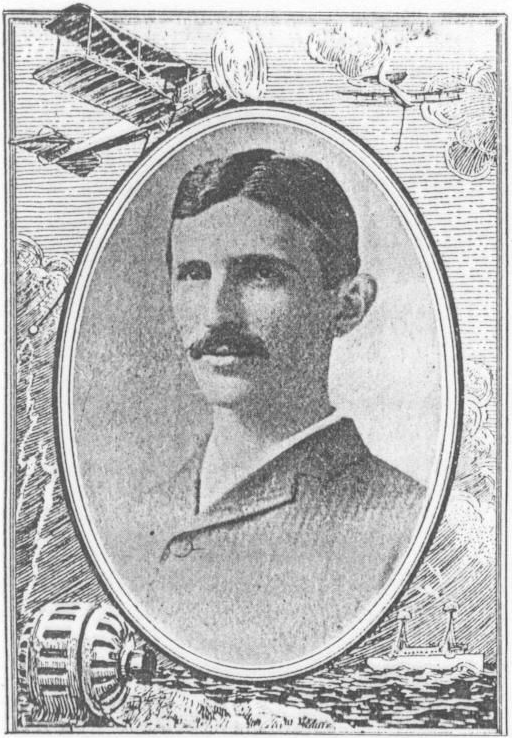
\includegraphics[width=\textwidth]{Tesla-29.png}
				%			\legend{Mr. Tesla at the Age of 29.}
			\end{minipage}}\hspace{1em}
			\adjustbox{valign=t}{\begin{minipage}[t]{.65\linewidth}
					\vspace*{1em}
					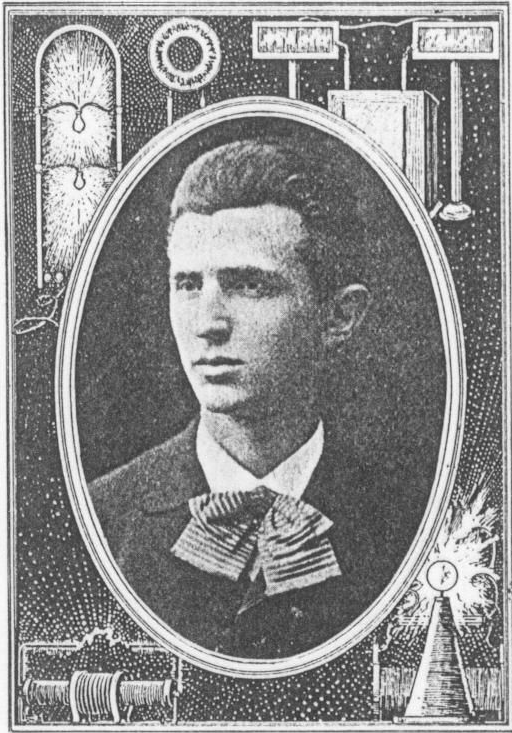
\includegraphics[width=\textwidth]{Tesla-23.png}
					\legend{Nikola Tesla at the Age of 23.}
				\end{minipage}}
			}
			
			\vspace*{1em}
			\makebox[\linewidth]{
				\noindent\adjustbox{valign=t}{\begin{minipage}{.65\linewidth}
						%		\vspace*{1em}	
						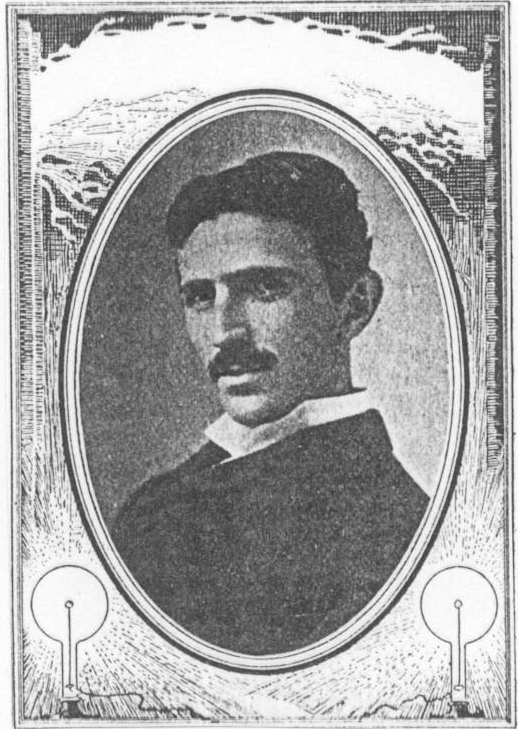
\includegraphics[width=\textwidth]{Tesla-39.png}
						\legend{Mr. Tesla at the Age of 39.}
					\end{minipage}}\hspace{1em}
					\adjustbox{valign=t}{\begin{minipage}{.65\linewidth}
							%			\noindent\begin{minipage}{\textwidth}
							\footnotesize\itshape\setlength{\columnsep}{.7em}
							\begin{multicols}{2}
								
								
								To begin, Tesla, who is birth a Serbian, comes from a long-lived hardy race. His family tree abounds with centenarians. Accordingly, Tesla -- barring accidents -- fully expects to be still inventing in A. D. 1960.
								
								But the chief reason for his perpetual youth is found in his gastronomical frugality. Tesla has learned the great fundamental truth that most people not only eat all of their bodily ills, but actually eat themselves to death by either eating too much or else by food that does not agree with them.
								
								When Tesla found out that tobacco and black coffee interfered with his physical well-being, he quit both. This is the simple menu of the great inventor:\\
								Breakfast: One to two pints of warm milk and a few eggs, prepared by himself -- yes he is a bachelor!\\
								Lunch: None whatsoever, as a rule.
								
								\columnbreak
								Dinner: Celery or the like, soupe, a single piece of meat or fowl, potatoes and one other vegetable; a glass of light wine. For desert, perhaps a slice of cheese, and invariably a big raw apple, and that's all.
								
								Tesla is very fussy and particular about his food: he eats very little, but what he does eat must be of the very best. And he knows, for outside of being a great inventor in science he is an accomplished cook who who has invented all sort of savory dishes.
								
								His only vice is his generosity. The man who, by the ignorant onlooker has often been called an idle dreamer, has made over a million dollars out of his inventions -- and spent them as quickly on new ones. But Tesla is an idealist of the highest order and to such men money itself means but little.
							\end{multicols}
							%			\end{minipage}
							
							%			\bigskip
							%		\centering\normalsize \itshape Mr. Nikola \textsc{Tesla}\\ at the Age of 23 (above), 29 (above right) and 39 (right).
						\end{minipage}}
					}
					\newpage
	
	
	\noindent -chanisms can be produced which will act as if possest of reason, to 
	a limited degree, and will create a revolution in many commercial and industrial departments.  
	
	I was about twelve years old when I first succeeded in banishing an image from my vision by 
	wilful effort, but I never had any control over the flashes of light to which I have referred.  They 
	were, perhaps, my strangest experience and inexplicable.  They usually occurred when I found 
	myself in a dangerous or distressing situation, or when I was greatly exhilarated.  In some 
	instances I have seen all the air around me filled with tongues of living flame.  Their intensity, 
	instead of diminishing, increased with time and seemingly attained a maximum when I was about 
	twenty-five years old.  While in Paris, in 1883, a prominent French manufacturer sent me an 
	invitation to a shooting expedition which I accepted.  I had been long confined to the factory and 
	the fresh air had a wonderfully invigorating effect on me.  On my return to the city that night I felt a 
	positive sensation that my brain had caught fire.  I saw a light as tho a small sun was located in it 
	and I past the whole night applying cold compressions to my tortured head.  Finally the flashes 
	diminished in frequency and force but it took more than three weeks before they wholly subsided.  
	When a second invitation was extended to me my answer was an emphatic NO! 
	
	These luminous phenomena still manifest themselves from time to time, as when a new idea 
	opening up possibilities strikes me, but they are no longer exciting, being of relatively small 
	intensity.  When I close my eyes I invariably observe first, a background of very dark and uniform 
	blue, not unlike the sky on a clear but starless night.  In a few seconds this field becomes 
	animated with innumerable scintillating flakes of green, arranged in several layers and advancing 
	towards me.  Then there appears, to the right, a beautiful pattern of two systems of parallel and 
	closely spaced lines, at right angles to one another, in all sorts of colors with yellow-green and 
	gold predominating.  Immediately thereafter the lines grow brighter and the whole is thickly 
	sprinkled with dots of twinkling light.  This picture moves slowly across the field of vision and in 
	about ten seconds vanishes to the left, leaving behind a ground of rather unpleasant and inert 
	grey which quickly gives way to a billowy sea of clouds, seemingly trying to mould themselves in 
	living shapes.  It is curious that I cannot project a form into this grey until the second phase is 
	reached.  Every time, before falling asleep, images of persons or objects flit before my view.  
	When I see them I know that I am about to lose consciousness.  If they are absent and refuse to 
	come it means a sleepless night.  
	
	To what an extent imagination played a part in my early life I may illustrate by another odd 
	experience.  Like most children I was fond of jumping and developed an intense desire to support 
	myself in the air.  Occasionally a strong wind richly charged with oxygen blew from the mountains 
	rendering my body as light as cork and then I would leap and float in space for a long time.  It was 
	a delightful sensation and my disappointment was keen when later I undeceived myself.  
	
	During that period I contracted many strange likes, dislikes and habits, some of which I can trace 
	to external impressions while others are unaccountable.  I had a violent aversion against the 
	earrings of women but other ornaments, as bracelets, pleased me more or less according to 
	design.  The sight of a pearl would almost give me a fit but I was fascinated with the glitter of 
	crystals or objects with sharp edges and plane surfaces.  I would not touch the hair of other 
	people except, perhaps, at the point of a revolver.  I would get a fever by looking at a peach and if 
	a piece of camphor was anywhere in the house it caused me the keenest discomfort.  Even now I 
	am not insensible to some of these upsetting impulses.  When I drop little squares of paper in a 
	dish filled with liquid, I always sense a peculiar and awful taste in my mouth.  I counted the steps 
	in my walks and calculated the cubical contents of soup plates, coffee cups and pieces of food—
	otherwise my meal was unenjoyable.  All repeated acts or operations I performed had to be 
	divisible by three and if I mist I felt impelled to do it all over again, even if it took hours.  
	
	Up to the age of eight years, my character was weak and vacillating.  I had neither courage or 
	strength to form a firm resolve.  My feelings came in waves and surges and vibrated unceasingly 
	between extremes.  My wishes were of consuming force and like the heads of the hydra, they 
	multiplied.  I was opprest by thoughts of pain in life and death and religious fear.  I was swayed by 
	superstitious belief and lived in constant dread of the spirit of evil, of ghosts and ogres and other 
	unholy monsters of the dark.  Then, all at once, there came a tremendous change which altered 
	the course of my whole existence.  Of all things I liked books the best.  My father had a large 
	library and whenever I could manage I tried to satisfy my passion for reading.  He did not permit it 
	and would fly into a rage when he caught me in the act.  He hid the candles when he found that I 
	was reading in secret.  He did not want me to spoil my eyes.  But I obtained tallow, made the 
	wicking and cast the sticks into tin forms, and every night I would bush the keyhole and the 
	cracks and read, often till dawn, when all others slept and my mother started on her arduous daily 
	task.  On one occasion I came across a novel entitled "Abafi" (the Son of Aba), a Serbian 
	translation of a well known Hungarian writer, Josika.  This work somehow awakened my dormant 
	powers of will and I began to practise self-control.  At first my resolutions faded like snow in April, 
	but in a little while I conquered my weakness and felt a pleasure I never knew before—that of 
	doing as I willed.  In the course of time this vigorous mental exercise became second nature.  At 
	the outset my wishes had to be subdued but gradually desire and will grew to be identical.  After 
	years of such discipline I gained so complete a mastery over myself that I toyed with passions 
	which have meant destruction to some of the strongest men.  At a certain age I contracted a 
	mania for gambling which greatly worried my parents.  To sit down to a game of cards was for me 
	the quintessence of pleasure.  My father led an exemplary life and could not excuse the 
	senseless waste of time and money in which I indulged.  I had a strong resolve but my philosophy 
	was bad.  I would say to him, "I can stop whenever I please but is it worth while to give up that 
	which I would purchase with the joys of Paradise?" On frequent occasions he gave vent to his 
	anger and contempt but my mother was different.  She understood the character of men and 
	knew that one's salvation could only be brought about thru his own efforts.  One afternoon, I 
	remember, when I had lost all my money and was craving for a game, she came to me with a roll 
	of bills and said, "Go and enjoy yourself.  The sooner you lose all we possess the better it will be.  
	I know that you will get over it." She was right.  I conquered my passion then and there and only 
	regretted that it had not been a hundred times as strong.  I not only vanquished but tore it from 
	my heart so as not to leave even a trace of desire.  Ever since that time I have been as indifferent 
	to any form of gambling as to picking teeth.  
	
	During another period I smoked excessively, threatening to ruin my health.  Then my will asserted 
	itself and I not only stopt but destroyed all inclination.  Long ago I suffered from heart trouble until 
	I discovered that it was due to the innocent cup of coffee I consumed every morning.  I 
	discontinued at once, tho I confess it was not an easy task.  In this way I checked and bridled 
	other habits and passions and have not only preserved my life but derived an immense amount of 
	satisfaction from what most men would consider privation and sacrifice.  
	
	After finishing the studies at the Polytechnic Institute and University I had a complete nervous 
	breakdown and while the malady lasted I observed many phenomena strange and unbelievable.

	
	\vspace*{\stretch{1}}
	{\centering
		\aldine\\
		\aldine\hspace{1.2em}\aldine
		\par}
	\vspace*{2cm}
	
	
%%------------------Chapitre 2 ------------------
	\cleardoublepage
	\thispagestyle{empty}
	\markboth{My First Efforts At Invention}{}
	\vspace*{5em}
	\begin{center}
		\bfseries
		\noindent {\Large\decofourleft~\textsc{II}~\decofourright}\\
		\noindent\rule{.5\linewidth}{1pt}\\
		\medskip
		{\noindent\LARGE My First Efforts \\At Invention}
		
		\bigskip
		
	
	{\normalfont\smallskip\small\protect\parbox{.75\linewidth}{\itshape
			\lettrine[lines=2]{B}{oys} will be boys, the world over. The Boy Tesla was no exception to the universal rule, as this, his second autobiographical article clearly proves.
			
			Mr. Tesla in his own inimitable, delightful way, here paints with a literary artist's brush his own intimate boyhodd in charming as well as vivid colors.
			
			We have often heard of Tesla, the dreamer. But if he is entitled to the epithet, his early boyhood certainly fails to reveal it. Tesla did not allow much grass to grow under his feet while a boy, for he assuredly was a strenuous, red-blooded youngster.
			
			You will wish to read all about the greatest inventor's early boyhood. It is doubly valuable because it comes from his own pen. We promise you an interesting twnty-minutes' entertainment.\\
			
			\hfill --\scshape{Editor}.
		}
		\par
	}

		\vspace*{5em}
	\end{center}
	
	\addtocontents{toc}{\normalsize}
	\addcontentsline{toc}{section}{My First Efforts At Invention}
	
	
	\lettrine[lines=3]{I}{} shall dwell briefly on these extraordinary experiences, on account of their possible interest to 
	students of psychology and physiology and also because this period of agony was of the greatest 
	consequence on my mental development and subsequent labors.  But it is indispensable to first 
	relate the circumstances and conditions which preceded them and in which might be found their 
	partial explanation.  
	
	From childhood I was compelled to concentrate attention upon myself.  This caused me much 
	suffering but, to my present view, it was a blessing in disguise for it has taught me to appreciate 
	the inestimable value of introspection in the preservation of life, as well as a means of 
	achievement.  The pressure of occupation and the incessant stream of impressions pouring into 
	our consciousness thru all the gateways of knowledge make modern existence hazardous in 
	many ways.  Most persons are so absorbed in the contemplation of the outside world that they 
	are wholly oblivious to what is passing on within themselves.  
	
	The premature death of millions is primarily traceable to this cause.  Even among those who 
	exercise care it is a common mistake to avoid imaginary, and ignore the real dangers.  And what 
	is true of an individual also applies, more or less, to a people as a whole.  Witness, in illustration, 
	the prohibition movement.  A drastic, if not unconstitutional, measure is now being put thru in this 
	country to prevent the consumption of alcohol and yet it is a positive fact that coffee, tea, tobacco, 
	chewing gum and other stimulants, which are freely indulged in even at the tender age, are vastly 
	more injurious to the national body, judging from the number of those who succumb.  So, for 
	instance, during my student years I gathered from the published necrologues in Vienna, the home 
	of coffee drinkers, that deaths from heart trouble sometimes reached sixty-seven per cent of the 
	total.  Similar observations might probably be made in cities where the consumption of tea is 
	excessive.  These delicious beverages superexcite and gradually exhaust the fine fibers of the 
	brain.  They also interfere seriously with arterial circulation and should be enjoyed all the more 
	sparingly as their deleterious effects are slow and imperceptible.  Tobacco, on the other hand, is 
	conducive to easy and pleasant thinking and detracts from the intensity and concentration 
	necessary to all original and vigorous effort of the intellect.  Chewing gum is helpful for a short 
	while but soon drains the glandular system and inflicts irreparable damage, not to speak of the 
	revulsion it creates.  Alcohol in small quantities is an excellent tonic, but is toxic in its action when 
	absorbed in larger amounts, quite immaterial as to whether it is taken in as whiskey or produced 
	in the stomach from sugar.  But it should not be overlooked that all these are great eliminators 
	assisting Nature, as they do, in upholding her stern but just law of the survival of the fittest.  Eager 
	reformers should also be mindful of the eternal perversity of mankind which makes the indifferent 
	"laissez-faire" by far preferable to enforced restraint.  


	The truth about this is that we need stimulants to do our best work under present living 
	conditions, and that we must exercise moderation and control our appetites and inclinations in 
	every direction.  That is what I have been doing for many years, in this way maintaining myself 
	young in body and mind.  Abstinence was not always to my liking but I find ample reward in the 
	agreeable experiences I am now making.  Just in the hope of converting some to my precepts 
	and convictions I will recall one or two.  
	
	A short time ago I was returning to my hotel.  It was a bitter cold night, the ground slippery, and 
	no taxi to be had.  Half a block behind me followed another man, evidently as anxious as myself 
	to get under cover.  Suddenly my legs went up in the air.  In the same instant there was a flash in 
	my brain, the nerves responded, the muscles contracted, I swung thru 180 degrees and landed 
	on my hands.  I resumed my walk as tho nothing had happened when the stranger caught up with 
	me.  "How old are you?" he asked, surveying me critically.  "Oh, about fifty-nine," I replied.  "What 
	of it?" "Well," said he, "I have seen a cat do this but never a man."  About a month since I wanted 
	to order new eyeglasses and went to an oculist who put me thru the usual tests.  He lookt at me 
	incredulously as I read off with ease the smallest print at considerable distance.  But when I told 
	him that I was past sixty he gasped in astonishment.  Friends of mine often remark that my suits 
	fit me like gloves but they do not know that all my clothing is made to measurements which were 
	taken nearly 35 years ago and never changed.  During this same period my weight has not varied 
	one pound.  
	
	In this connection I may tell a funny story.  One evening, in the winter of 1885, Mr. Edison, 
	Edward H. Johnson, the President of the Edison Illuminating Company, Mr. Batchellor, Manager 
	of the works, and myself entered a little place opposite 65 Fifth Avenue where the offices of the 
	company were located.  Someone suggested guessing weights and I was induced to step on a 
	scale.  Edison felt me all over and said: "Tesla weighs 152 lbs.  to an ounce," and he guest it 
	exactly.  Stript I weighed 142 lbs.  and that is still my weight.  I whispered to Mr. Johnson: "How is 
	it possible that Edison could guess my weight so closely?" "Well," he said, lowering his voice.  "I 
	will tell you, confidentially, but you must not say anything.  He was employed for a long time in a 
	Chicago slaughter-house where he weighed thousands of hogs every day! That's why." My friend, 
	the Hon. Chauncey M. Depew, tells of an Englishman on whom he sprung one of his original 
	anecdotes and who listened with a puzzled expression but - a year later - laughed out loud.  I will 
	frankly confess it took me longer than that to appreciate Johnson's joke.  
	
%	{\bigskip
		\begin{figure}[b]
		\centering
		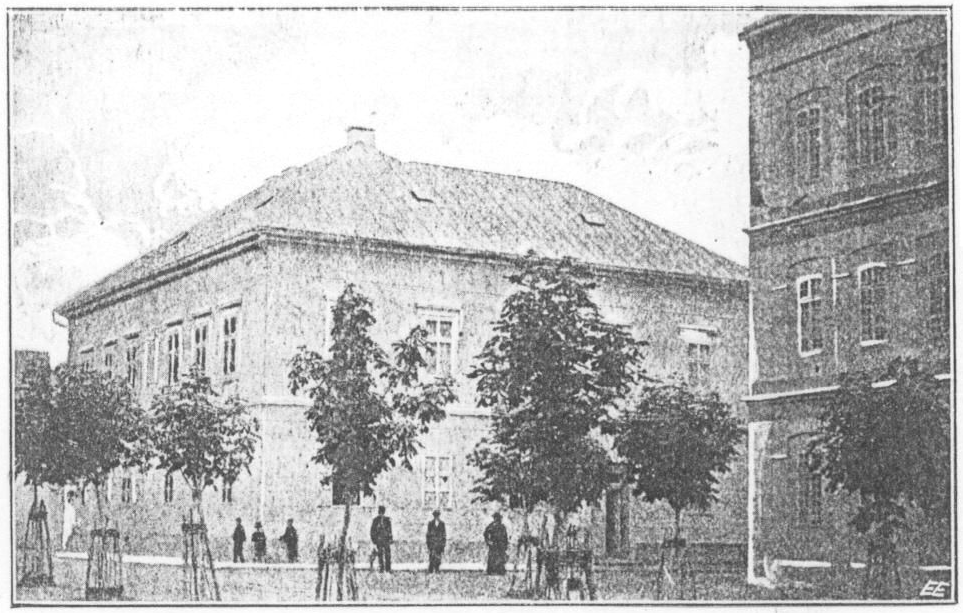
\includegraphics[width=.75\textwidth]{House.png}
%		\captionsetup{width=.75\textwidth}
		\legend{This Photograph Shows in the Background the House in Which Mr. Teslas' Family Resided. The Edifice at the Right is the "Real-Gymnasium" Where he Studied. The Eccleclastic Gentleman is his Uncle, the Metropolitan of Bosnia, Who was a Great Stateman and Who Thwarted the Design of Austria Upon the Serbia at a Critical Period.}
		\end{figure}
%		\par
%		\medskip}
	
	Now, my well being is simply the result of a careful and measured mode of living and perhaps the 
	most astonishing thing is that three times in my youth I was rendered by illness a hopeless 
	physical wreck and given up by physicians.  More than this, thru ignorance and lightheartedness, 
	I got into all sorts of difficulties, dangers and scrapes from which I extricated myself as by 
	enchantment.  I was almost drowned a dozen times; was nearly boiled alive and just mist being 
	cremated.  I was entombed, lost and frozen.  I had hair-breadth escapes from mad dogs, hogs, 
	and other wild animals.  I past thru dreadful diseases and met with all kinds of odd mishaps and 
	that I am hale and hearty today seems like a miracle.  But as I recall these incidents to my mind I 
	feel convinced that my preservation was not altogether accidental.  
	
	An inventor's endeavor is essentially lifesaving.  Whether he harnesses forces, improves devices, 
	or provides new comforts and conveniences, he is adding to the safety of our existence.  He is 
	also better qualified than the average individual to protect himself in peril, for he is observant and 
	resourceful.  If I had no other evidence that I was, in a measure, possest of such qualities I would 
	find it in these personal experiences.  The reader will be able to judge for himself if I mention one 
	or two instances.  On one occasion, when about 14 years old, I wanted to scare some friends 
	who were bathing with me.  My plan was to dive under a long floating structure and slip out 
	quietly at the other end.  Swimming and diving came to me as naturally as to a duck and I was 
	confident that I could perform the feat.  Accordingly I plunged into the water and, when out of 
	view, turned around and proceeded rapidly towards the opposite side.  Thinking that I was safely 
	beyond the structure, I rose to the surface but to my dismay struck a beam.  Of course, I quickly 
	dived and forged ahead with rapid strokes until my breath was beginning to give out.  Rising for 
	the second time, my head came again in contact with a beam.  Now I was becoming desperate.  
	However, summoning all my energy, I made a third frantic attempt but the result was the same.  
	The torture of supprest breathing was getting unendurable, my brain was reeling and I felt myself 
	sinking.  At that moment, when my situation seemed absolutely hopeless, I experienced one of 
	those flashes of light and the structure above me appeared before my vision.  I either discerned 
	or guest that there was a little space between the surface of the water and the boards resting on 
	the beams and, with consciousness nearly gone, I floated up, prest my mouth close to the planks 
	and managed to inhale a little air, unfortunately mingled with a spray of water which nearly 
	choked me.  Several times I repeated this procedure as in a dream until my heart, which was 
	racing at a terrible rate, quieted down and I gained composure.  After that I made a number of 
	unsuccessful dives, having completely lost the sense of direction, but finally succeeded in getting 
	out of the trap when my friends had already given me up and were fishing for my body.  
	
	That bathing season was spoiled for me thru recklessness but I soon forgot the lesson and only 
	two years later I fell into a worse predicament.  There was a large flour mill with a dam across the 
	river near the city where I was studying at that time.  As a rule the height of the water was only 
	two or three inches above the dam and to swim out to it was a sport not very dangerous in which I 
	often indulged.  One day I went alone to the river to enjoy myself as usual.  When I was a short 
	distance from the masonry, however, I was horrified to observe that the water had risen and was 
	carrying me along swiftly.  I tried to get away but it was too late.  Luckily, tho, I saved myself from 
	being swept over by taking hold of the wall with both hands.  The pressure against my chest was 
	great and I was barely able to keep my head above the surface.  Not a soul was in sight and my 
	voice was lost in the roar of the fall.  Slowly and gradually I became exhausted and unable to 
	withstand the strain longer.  just as I was about to let go, to be dashed against the rocks below, I 
	saw in a flash of light a familiar diagram illustrating the hydraulic principle that the pressure of a 
	fluid in motion is proportionate to the area exposed, and automatically I turned on my left side.  As 
	if by magic the pressure was reduced and I found it comparatively easy in that position to resist 
	the force of the stream.  But the danger still confronted me.  I knew that sooner or later I would be 
	carried down, as it was not possible for any help to reach me in time, even if I attracted attention.  
	I am ambidextrous now but then I was lefthanded and had comparatively little strength in my right 
	arm.  For this reason I did not dare to turn on the other side to rest and nothing remained but to 
	slowly push my body along the dam.  I had to get away from the mill towards which my face was 
	turned as the current there was much swifter and deeper.  It was a long and painful ordeal and I 
	came near to failing at its very end for I was confronted with a depression in the masonry.  I 
	managed to get over with the last ounce of my force and fell in a swoon when I reached the bank, 
	where I was found.  I had torn virtually all the skin from my left side and it took several weeks 
	before the fever subsided and I was well.  These are only two of many instances but they may be 
	sufficient to show that had it not been for the inventor's instinct I would not have lived to tell this 
	tale.  
	
	Interested people have often asked me how and when I began to invent.  This I can only answer 
	from my present recollection in the light of which the first attempt I recall was rather ambitious for 
	it involved the invention of an apparatus and a method.  In the former I was anticipated but the 
	latter was original.  It happened in this way.  One of my playmates had come into the possession 
	of a hook and fishing-tackle which created quite an excitement in the village, and the next 
	morning all started out to catch frogs.  I was left alone and deserted owing to a quarrel with this 
	boy.  I had never seen a real hook and pictured it as something wonderful, endowed with peculiar 
	qualities, and was despairing not to be one of the party.  Urged by necessity, I somehow got hold 
	of a piece of soft iron wire, hammered the end to a sharp point between two stones, bent it into 
	shape, and fastened it to a strong string.  I then cut a rod, gathered some bait, and went down to 
	the brook where there were frogs in abundance.  But I could not catch any and was almost 
	discouraged when it occurred to me to dangle the empty hook in front of a frog sitting on a stump.  
	At first he collapsed but by and by his eyes bulged out and became bloodshot, he swelled to 
	twice his normal size and made a vicious snap at the hook.  
	
	Immediately I pulled him up.  I tried the same thing again and again and the method proved 
	infallible.  When my comrades, who in spite of their fine outfit had caught nothing, came to me 
	they were green with envy.  For a long time I kept my secret and enjoyed the monopoly but finally 
	yielded to the spirit of Christmas.  Every boy could then do the same and the following summer 
	brought disaster to the frogs.  
	
	In my next attempt I seem to have acted under the first instinctive impulse which later dominated 
	me - to harness the energies of nature to the service of man.  I did this thru the medium of May-
	bugs - or June-bugs as they are called in America - which were a veritable pest in that country 
	and sometimes broke the branches of trees by the sheer weight of their bodies.  The bushes 
	were black with them.  I would attach as many as four of them to a crosspiece, rotably arranged 
	on a thin spindle, and transmit the motion of the same to a large disc and so derive considerable 
	"power." These creatures were remarkably efficient, for once they were started they had no sense 
	to stop and continued whirling for hours and hours and the hotter it was the harder they worked.  
	All went well until a strange boy came to the place.  He was the son of a retired officer in the 
	Austrian Army.  That urchin ate May-bugs alive and enjoyed them as tho they were the finest 
	blue-point oysters.  That disgusting sight terminated my endeavors in this promising field and I 
	have never since been able to touch a May-bug or any other insect for that matter.  
	
	After that, I believe, I undertook to take apart and assemble the clocks of my grandfather.  In the 
	former operation I was always successful but often failed in the latter.  So it came that he brought 
	my work to a sudden halt in a manner not too delicate and it took thirty years before I tackled 
	another clockwork again.  Shortly there after I went into the manufacture of a kind of pop-gun 
	which comprised a hollow tube, a piston, and two plugs of hemp.  When firing the gun, the piston 
	was prest against the stomach and the tube was pushed back quickly with both hands.  The air 
	between the plugs was comprest and raised to high temperature and one of them was expelled 
	with a loud report.  The art consisted in selecting a tube of the proper taper from the hollow stalks.  
	I did very well with that gun but my activities interfered with the window panes in our house and 
	met with painful discouragement.  If I remember rightly, I then took to carving swords from pieces 
	of furniture which I could conveniently obtain.  At that time I was under the sway of the Serbian 
	national poetry and 
	
	\begin{figure}[p]
	\vspace*{-2cm}
	\makebox[\linewidth]{
		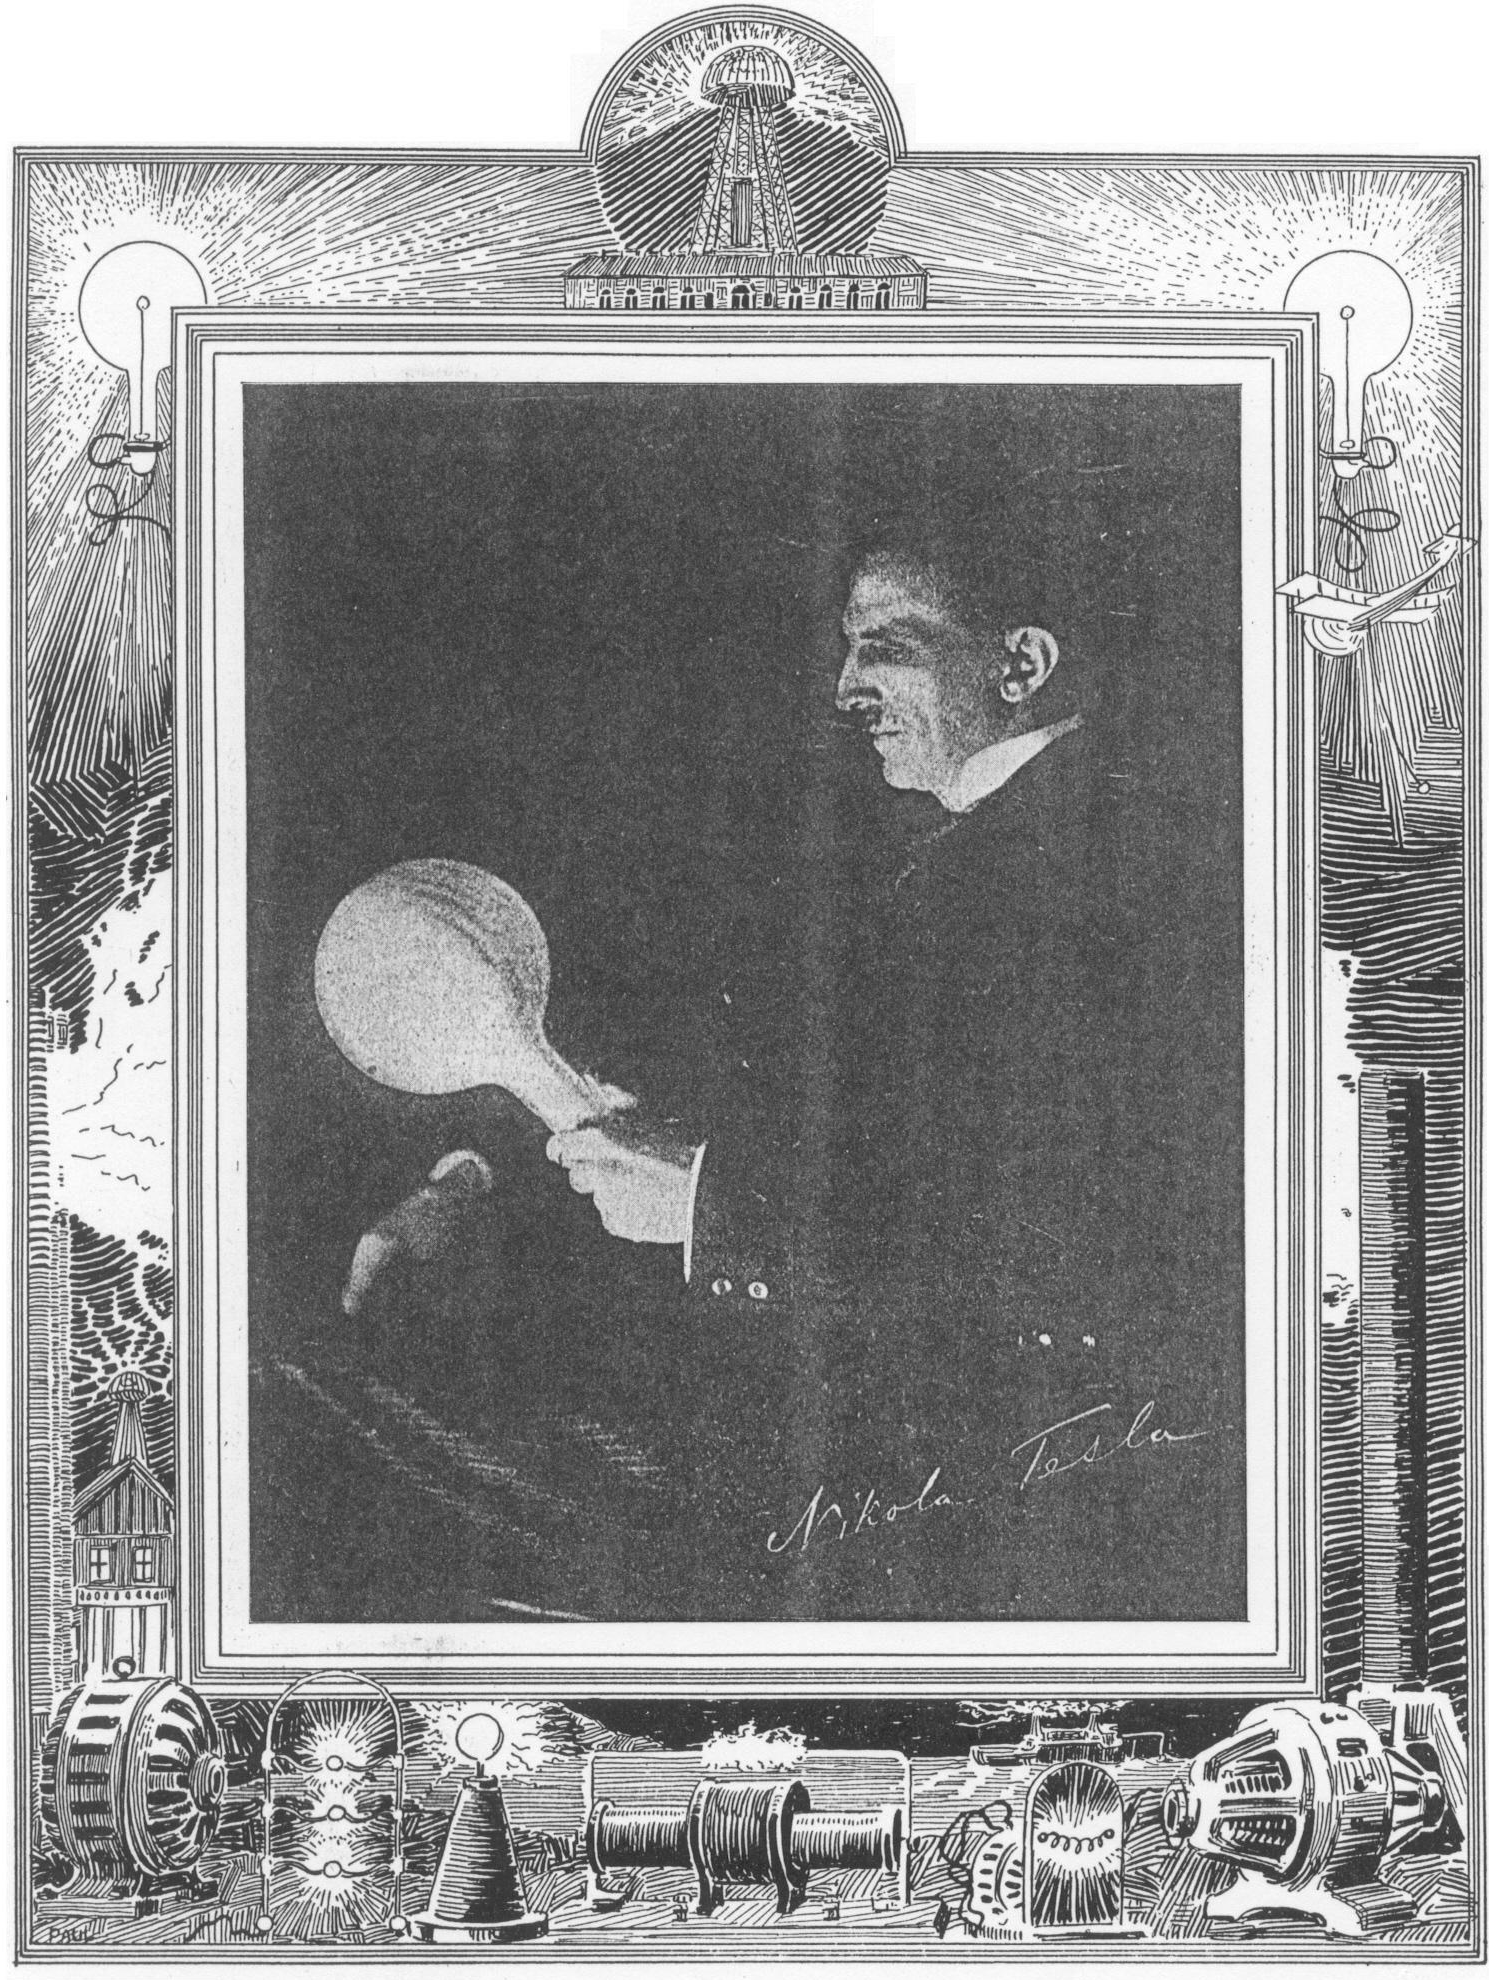
\includegraphics[width=1.3\linewidth]{Tesla-bulbe.png}
		}
		\legend{An Interesting Study of the Great Inventor Contemplating the Glass Buble of his Famous Wireless Light. A Full Description of the Invention will Appear Shortly in the \textsc{Electrical Experimenter}. This is the Only Profile Photograph of Mr. Tesla in Existence. It was Taken Specially for the \textsc{Electrical Experimenter}.}
	\end{figure}
%	{\centering
%	\vspace{\stretch{1}}
%	
%	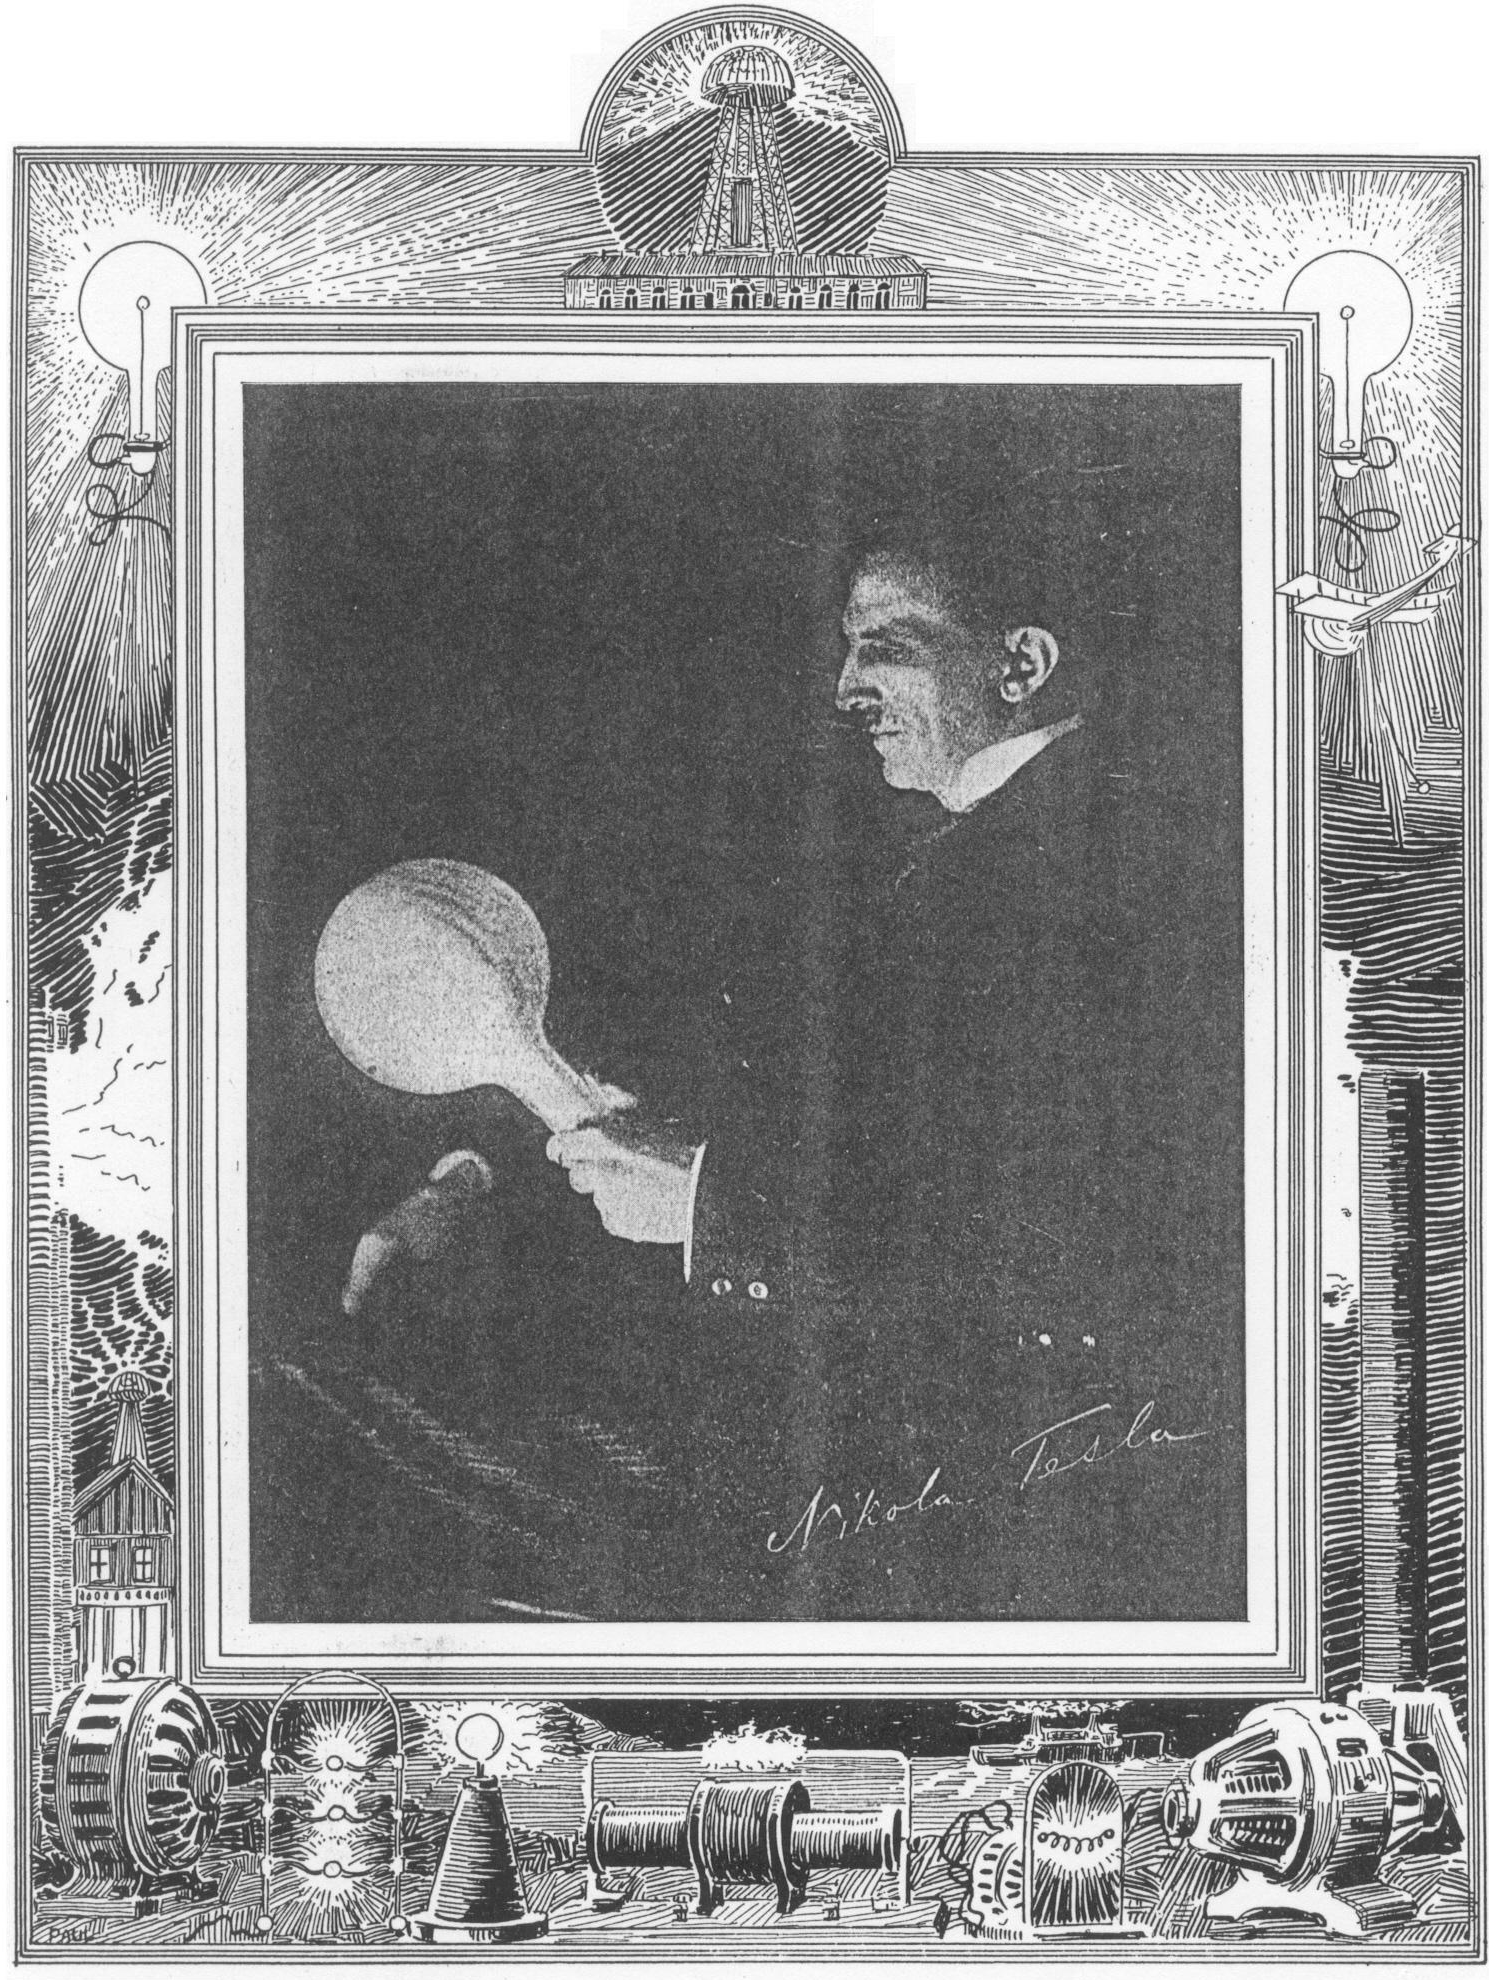
\includegraphics[width=\textwidth]{Tesla-bulbe.png}
%	
%	\vspace{\stretch{1}}
%	\par
%	}
%	\newpage
	
	
	\noindent full of admiration for the feats of the heroes.  I used to spend hours in mowing 
	down my enemies in the form of corn-stalks which ruined the crops and netted me several 
	spankings from my mother.  Moreover these were not of the formal kind but the genuine article.  
	
	
	I had all this and more behind me before I was six years old and had past thru one year of 
	elementary school in the village of Smiljan where I was born.  At this juncture we moved to the 
	little city of Gospic nearby.  This change of residence was like a calamity to me.  It almost broke 
	my heart to part from our pigeons, chickens and sheep, and our magnificent flock of geese which 
	used to rise to the clouds in the morning and return from the feeding grounds at sundown in battle 
	formation, so perfect that it would have put a squadron of the best aviators of the present day to 
	shame.  In our new house I was but a prisoner, watching the strange people I saw thru the 
	window blinds.  My bashfulness was such that I would rather have faced a roaring lion than one 
	of the city dudes who strolled about.  But my hardest trial came on Sunday when I had to dress 
	up and attend the service.  There I meet with an accident, the mere thought of which made my 
	blood curdle like sour milk for years afterwards.  It was my second adventure in a church.  Not 
	long before I was entombed for a night in an old chapel on an inaccessible mountain which was 
	visited only once a year.  It was an awful experience, but this one was worse.  There was a 
	wealthy lady in town, a good but pompous woman, who used to come to the church gorgeously 
	painted up and attired with an enormous train and attendants.  One Sunday I had just finished 
	ringing the bell in the belfry and rushed downstairs when this grand dame was sweeping out and I 
	jumped on her train.  It tore off with a ripping noise which sounded like a salvo of musketry fired 
	by raw recruits.  My father was livid with rage.  He gave me a gentle slap on the cheek, the only 
	corporal punishment he ever administered to me but I almost feel it now.  The embarrassment 
	and confusion that followed are indescribable.  I was practically ostracised until something else 
	happened which redeemed me in the estimation of the community.  
	
	An enterprising young merchant had organized a fire department.  A new fire engine was 
	purchased, uniforms provided and the men drilled for service and parade.  The engine was, in 
	reality, a pump to be worked by sixteen men and was beautifully painted red and black.  One 
	afternoon the official trial was prepared for and the machine was transported to the river.  The 
	entire population turned out to witness the great spectacle.  When all the speeches and 
	ceremonies were concluded, the command was given to pump, but not a drop of water came 
	from the nozzle.  The professors and experts tried in vain to locate the trouble.  The fizzle was 
	complete when I arrived at the scene.  My knowledge of the mechanism was nil and I knew next 
	to nothing of air pressure, but instinctively I felt for the suction hose in the water and found that it 
	had collapsed.  When I waded in the river and opened it up the water rushed forth and not a few 
	Sunday clothes were spoiled.  Archimedes running naked thru the streets of Syracuse and 
	shouting Eureka at the top of his voice did not make a greater impression than myself.  I was 
	carried on the shoulders and was the hero of the day.  
	
	Upon settling in the city I began a four-years' course in the so-called Normal School preparatory 
	to my studies at the College or Real Gymnasium.  During this period my boyish efforts and 
	exploits, as well as troubles, continued.  Among other things I attained the unique distinction of 
	champion crow catcher in the country.  My method of procedure was extremely simple.  I would 
	go in the forest, hide in the bushes, and imitate the call of the bird.  Usually I would get several 
	answers and in a short while a crow would flutter down into the shrubbery near me.  After that all I 
	needed to do was to throw a piece of cardboard to distract its attention, jump up and grab it 
	before it could extricate itself from the undergrowth.  In this way I would capture as many as I 
	desired.  But on one occasion something occurred which made me respect them.  I had caught a 
	fine pair of birds and was returning home with a friend.  When we left the forest, thousands of 
	crows had gathered making a frightful racket.  In a few minutes they rose in pursuit and soon 
	enveloped us.  The fun lasted until all of a sudden I received a blow on the back of my head 
	which knocked me down.  Then they attacked me viciously.  I was compelled to release the two 
	birds and was glad to join my friend who had taken refuge in a cave.  
	
	In the schoolroom there were a few mechanical models which interested me and turned my 
	attention to water turbines.  I constructed many of these and found great pleasure in operating 
	them.  How extraordinary was my life an incident may illustrate.  My uncle had no use for this kind 
	of pastime and more than once rebuked me.  I was fascinated by a description of Niagara Falls I 
	had perused, and pictured in my imagination a big wheel run by the Falls.  I told my uncle that I 
	would go to America and carry out this scheme.  Thirty years later I saw my ideas carried out at 
	Niagara and marveled at the unfathomable mystery of the mind.  
	
	I made all kinds of other contrivances and contraptions but among these the arbalists I produced 
	were the best.  My arrows, when shot, disappeared from sight and at close range traversed a 
	plank of pine one inch thick.  Thru the continuous tightening of the bows I developed skin on my 
	stomach very much like that of a crocodile and I am often wondering whether it is due to this 
	exercise that I am able even now to digest cobble-stones! Nor can I pass in silence my 
	performances with the sling which would have enabled me to give a stunning exhibit at the 
	Hippodrome.  And now I will tell of one of my feats with this antique implement of war which will 
	strain to the utmost the credulity of the reader.  I was practicing while walking with my uncle along 
	the river.  The sun was setting, the trout were playful and from time to time one would shoot up 
	into the air, its glistening body sharply defined against a projecting rock beyond.  Of course any 
	boy might have hit a fish under these propitious conditions but I undertook a much more difficult 
	task and I foretold to my uncle, to the minutest detail, what I intended doing.  I was to hurl a stone 
	to meet the fish, press its body against the rock, and cut it in two.  It was no sooner said than 
	done.  My uncle looked at me almost scared out of his wits and exclaimed "Vade retro Satanas!" 
	and it was a few days before he spoke to me again.  Other records, how ever great, will be 
	eclipsed but I feel that I could peacefully rest on my laurels for a thousand years.
	


	\vspace*{\stretch{1}}
	{\centering
		\aldine\\
		\aldine\hspace{1.2em}\aldine
		\par}
	\vspace*{2cm}
	


%%------------------Chapitre 3 ------------------
\cleardoublepage
\thispagestyle{empty}
\markboth{My Later Endeavors}{}
\vspace*{5em}
\begin{center}
	\bfseries
	\noindent {\Large\decofourleft~\textsc{III}~\decofourright}\\
	\noindent\rule{.5\linewidth}{1pt}\\
	\medskip
	{\noindent\LARGE My Later\\Endeavors\\}{\medskip \normalsize \normalfont The Discovery of the Rotating Magnetic Field}
	
	\bigskip
	
	{\normalfont\smallskip\footnotesize\protect\parbox{.75\linewidth}{\itshape
			\lettrine[lines=2]{T}{his} installment, no doubt the most interesting of the three published so far, reveals many extraordinary occurences and experiences in the world greatest inventor's life -- experience such as do not fall to the lot of ordinary mortals. And Tesla, the many sided, aside of inventing, knows the rare art of painting world-pictures. He does so in a masterly fashion. He tell us how he finally conceived the induction motors -- perhaps his greatest discovery -- the invention which changed the face of the globe, the invention which made possible the street car, the subway, the electric train, power transmission, the harnessing of waterfalls and countless others. But let Tesla tell you himself how it all came about. It is a classic worth reading.\\
			
			\hfill --\scshape{Editor}.
			}
		\par
	}
	\vspace*{5em}
\end{center}

\addtocontents{toc}{\normalsize}
\addcontentsline{toc}{section}{My Later Endeavors}



\lettrine[lines=3]{A}{t} the age of ten I entered the Real Gymnasium which was a new and fairly well equipt institution.  
In the department of physics were various models of classical scientific apparatus, electrical and 
mechanical.  The demonstrations and experiments performed from time to time by the instructors 
fascinated me and were undoubtedly a powerful incentive to invention.  I was also passionately 
fond of mathematical studies and often won the professor's praise for rapid calculation.  This was 
due to my acquired facility of visualizing the figures and performing the operations, not in the 
usual intuitive manner, but as in actual life.  Up to a certain degree of complexity it was absolutely 
the same to me whether I wrote the symbols on the board or conjured them before my mental 
vision.  But freehand drawing, to which many hours of the course were devoted, was an 
annoyance I could not endure.  This was rather remarkable as most of the members of the family 
excelled in it.  Perhaps my aversion was simply due to the predilection I found in undisturbed 
thought.  Had it not been for a few exceptionally stupid boys, who could not do anything at all, my 
record would have been the worst.  It was a serious handicap as under the then existing 
educational regime, drawing being obligatory, this deficiency threatened to spoil my whole career 
and my father had considerable trouble in railroading me from one class to another.  

In the second year at that institution I became obsessed with the idea of producing continuous 
motion thru steady air pressure.  The pump incident, of which I have told, had set afire my 
youthful imagination and imprest me with the boundless abilities of a vacuum.  I grew frantic in my 
desire to harness this inexhaustible energy but for a long time I was groping in the dark.  Finally, 
however, my endeavors crystallized in an invention which was to enable me to achieve what no 
other mortal ever attempted.  

Imagine a cylinder freely rotatable on two bearings and partly surrounded by a rectangular trough 
which fits it perfectly.  The open side of the trough is closed by a partition so that the cylindrical 
segment within the enclosure divides the latter into two compartments entirely separated from 
each other by air-tight sliding joints.  One of these compartments being sealed and once for all 
exhausted, the other remaining open, a perpetual rotation of the cylinder would result, at least, I 
thought so.  A wooden model was constructed and fitted with infinite care and when I applied the 
pump on one side and actually observed that there was a tendency to turning, I was delirious with 
joy.  Mechanical flight was the one thing I wanted to accomplish altho still under the discouraging 
recollection of a bad fall I sustained by jumping with an umbrella from the top of a building.  Every 
day I used to transport myself thru the air to distant regions but could not understand just how I 
managed to do it.  Now I had something concrete—a flying machine with nothing more than a 
rotating shaft, flapping wings, and—a vacuum of unlimited power! From that time on I made my 
daily aerial excursions in a vehicle of comfort and luxury as might have befitted King Solomon.  It 
took years before I understood that the atmospheric pressure acted at right angles to the surface 
of the cylinder and that the slight rotary effort I observed was due to a leak.  Tho this knowledge 
came gradually it gave me a painful shock.  

I had hardly completed my course at the Real Gymnasium when I was prostrated with a 
dangerous illness or rather, a score of them, and my condition became so desperate that I was 
given up by physicians.  During this period I was permitted to read constantly, obtaining books 
from the Public Library which had been neglected and entrusted to me for classification of the 
works and preparation of the catalogues.  One day I was handed a few volumes of new literature 
unlike anything I had ever read before and so captivating as to make me utterly forget my 
hopeless state.  They were the earlier works of Mark Twain and to them might have been due the 
miraculous recovery which followed.  Twenty-five years later, when I met Mr. Clemens and we 
formed a friendship between us, I told him of the experience and was amazed to see that great 
man of laughter burst into tears.  

\begin{wrapfigure}{r}{0.65\textwidth}
	\vspace{-20pt}
	\begin{center}
		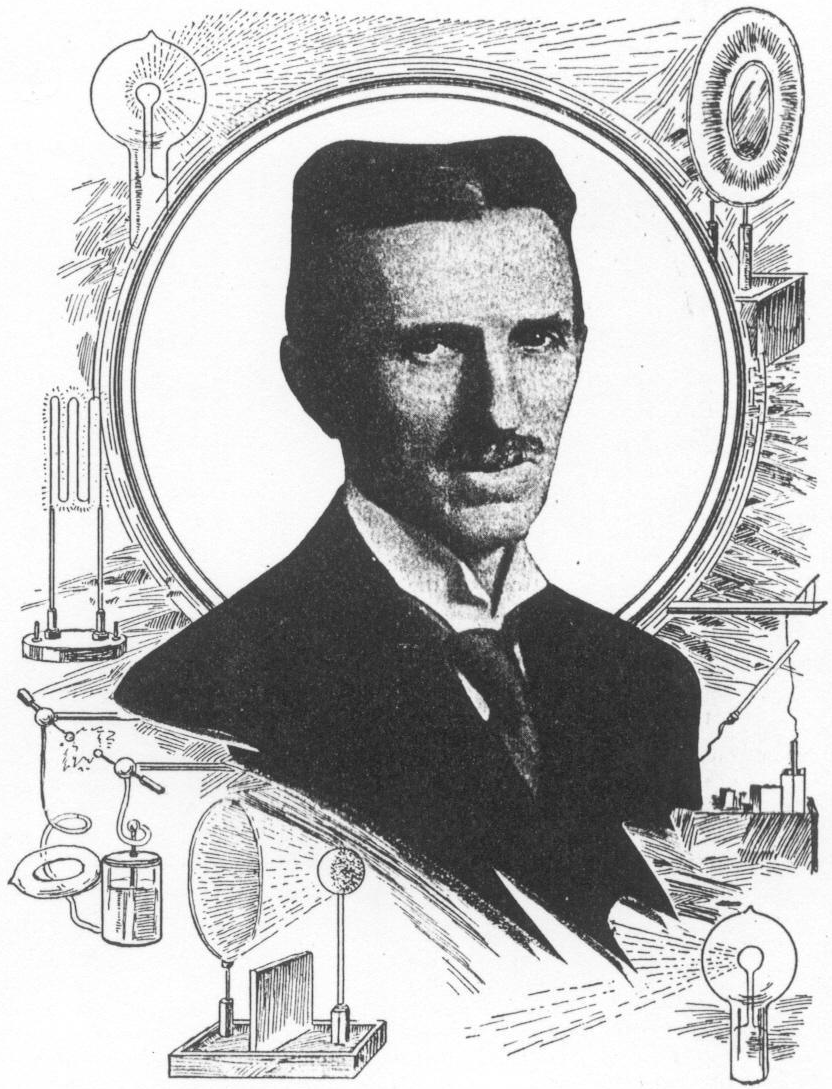
\includegraphics[width=0.63\textwidth]{Tesla-60.png}
	\end{center}
	\legend{Nikola Tesla at 60. A Very Recent Portrait of the Great Inventor. An Excellent Likeness.}
	\vspace{-20pt}
\end{wrapfigure}

My studies were continued at the higher Real Gymnasium in Carlstadt, Croatia, where one of my 
aunts resided.  She was a distinguished lady, the wife of a Colonel who was an old war-horse 
having participated in many battles.  I never can forget the three years I past at their home.  No 
fortress in time of war was under a more rigid discipline.  I was fed like a canary bird.  All the 
meals were of the highest quality and deliciously prepared but short in quantity by a thousand 
percent.  The slices of ham cut by my aunt were like tissue paper.  When the Colonel would put 
something substantial on my plate she would snatch it away and say excitedly to him: "Be careful, 
Niko is very delicate." I had a voracious appetite and suffered like Tantalus.  But I lived in an 
atmosphere of refinement and artistic taste quite unusual for those times and conditions.  The 
land was low and marshy and malaria fever never left me while there despite of the enormous 
amounts of quinin I consumed.  Occasionally the river would rise and drive an army of rats into 
the buildings, devouring everything even to the bundles of the fierce paprika.  These pests were 
to me a welcome diversion.  I thinned their ranks by all sorts of means, which won me the 
unenviable distinction of rat-catcher in the community.  At last, however, my course was 
completed, the misery ended, and I obtained the certificate of maturity which brought me to the 
cross-roads.  

During all those years my parents never wavered in their resolve to make me embrace the clergy, 
the mere thought of which filled me with dread.  I had become intensely interested in electricity 
under the stimulating influence of my Professor of Physics, who was an ingenious man and often 
demonstrated the principles by apparatus of his own invention.  Among these I recall a device in 
the shape of a freely rotatable bulb, with tinfoil coatings, which was made to spin rapidly when 
connected to a static machine.  It is impossible for me to convey an adequate idea of the intensity 
of feeling I experienced in witnessing his exhibitions of these mysterious phenomena.  Every 
impression produced a thousand echoes in my mind.  I wanted to know more of this wonderful 
force; I longed for experiment and investigation and resigned myself to the inevitable with aching 
heart.  

Just as I was making ready for the long journey home I received word that my father wished me 
to go on a shooting expedition.  It was a strange request as he had been always strenuously 
opposed to this kind of sport.  But a few days later I learned that the cholera was raging in that 
district and, taking advantage of an opportunity, I returned to Gospic in disregard of my parents' 
wishes.  It is incredible how absolutely ignorant people were as to the causes of this scourge 
which visited the country in intervals of from fifteen to twenty years.  They thought that the deadly 
agents were transmitted thru the air and filled it with pungent odors and smoke.  In the meantime 
they drank the infected water and died in heaps.  I contracted the awful disease on the very day 
of my arrival and altho surviving the crisis, I was confined to bed for nine months with scarcely 
any ability to move.  My energy was completely exhausted and for the second time I found myself 
at death's door.  In one of the sinking spells which was thought to be the last, my father rushed 
into the room.  I still see his pallid face as he tried to cheer me in tones belying his assurance.  
"Perhaps," I said, "I may get well if you will let me study engineering." "You will go to the best 
technical institution in the world," he solemnly replied, and I knew that he meant it.  A heavy 
weight was lifted from my mind but the relief would have come too late had it not been for a 
marvelous cure brought about thru a bitter decoction of a peculiar bean.  I came to life like 
another Lazarus to the utter amazement of everybody.  

My father insisted that I spend a year in healthful physical outdoor exercises to which I reluctantly 
consented.  For most of this term I roamed in the mountains, loaded with a hunter's outfit and a bundle of books, and this contact with nature made me stronger in body as well as in mind.  I 
thought and planned, and conceived many ideas almost as a rule delusive.  The vision was clear 
enough but the knowledge of principles was very limited.  In one of my inventions I proposed to 
convey letters and packages across the seas, thru a submarine tube, in spherical containers of 
sufficient strength to resist the hydraulic pressure.  The pumping plant, intended to force the 
water thru the tube, was accurately figured and designed and all other particulars carefully 
worked out.  Only one trifling detail, of no consequence, was lightly dismist.  I assumed an 
arbitrary velocity of the water and, what is more, took pleasure in making it high, thus arriving at a 
stupendous performance supported by faultless calculations.  Subsequent reflections, however, 
on the resistance of pipes to fluid flow determined me to make this invention public property.  

Another one of my projects was to construct a ring around the equator which would, of course, 
float freely and could be arrested in its spinning motion by reactionary forces, thus enabling travel 
at a rate of about one thousand miles an hour, impracticable by rail.  The reader will smile.  The 
plan was difficult of execution, I will admit, but not nearly so bad as that of a well-known New York 
professor, who wanted to pump the air from the torrid to the temperate zones, entirely forgetful of 
the fact that the Lord had provided a gigantic machine for this very purpose.  

Still another scheme, far more important and attractive, was to derive power from the rotational 
energy of terrestrial bodies.  I had discovered that objects on the earth's surface, owing to the 
diurnal rotation of the globe, are carried by the same alternately in and against the direction of 
translatory movement.  From this results a great change in momentum which could be utilized in 
the simplest imaginable manner to furnish motive effort in any habitable region of the world.  I 
cannot find words to describe my disappointment when later I realized that I was in the 
predicament of Archi\-medes, who vainly sought for a fixt point in the universe.


At the termination of my vacation I was sent to the Polytechnic School in Gratz, Styria, which my 
father had chosen as one of the oldest and best reputed institutions.  That was the moment I had 
eagerly awaited and I began my studies under good auspices and firmly resolved to succeed.  My 
previous training was above the average, due to my father's teaching and opportunities afforded.  
I had acquired the knowledge of a number of languages and waded thru the books of several 
libraries, picking up information more or less useful.  Then again, for the first time, I could choose 
my subjects as I liked, and free-hand drawing was to bother me no more.  

I had made up my mind to give my parents a surprise, and during the whole first year I regularly 
started my work at three o'clock in the morning and continued until eleven at night, no Sundays or 
holidays excepted.  As most of my fellow-students took thinks easily, naturally enough I eclipsed 
all records.  In the course of that year I past thru nine exams and the professors thought I 
deserved more than the highest qualifications.  Armed with their flattering certificates, I went 
home for a short rest, expecting a triumph, and was mortified when my father made light of these 
hard won honors.  That almost killed my ambition; but later, after he had died, I was pained to find 
a package of letters which the professors had written him to the effect that unless he took me 
away from the Institution I would be killed thru overwork.  

Thereafter I devoted myself chiefly to physics, mechanics and mathematical studies, spending 
the hours of leisure in the libraries.  I had a veritable rnania for finishing whatever I began, which 
often got me into difficulties.  On one occasion I started to read the works of Voltaire when I 
learned, to my dismay, that there were close on one hundred large volumes in small print which 
that monster had written while drinking seventy-two cups of black coffee per diem.  It had to be 
done, but when I laid aside the last book I was very glad, and said, "Never more!" 

My first year's showing had won me the appreciation and friendship of several professors. Among these were Prof. Rogner, who was teaching arithmetical 
\begin{wrapfigure}{r}{0.65\textwidth}
	\vspace{-20pt}
	\begin{center}
		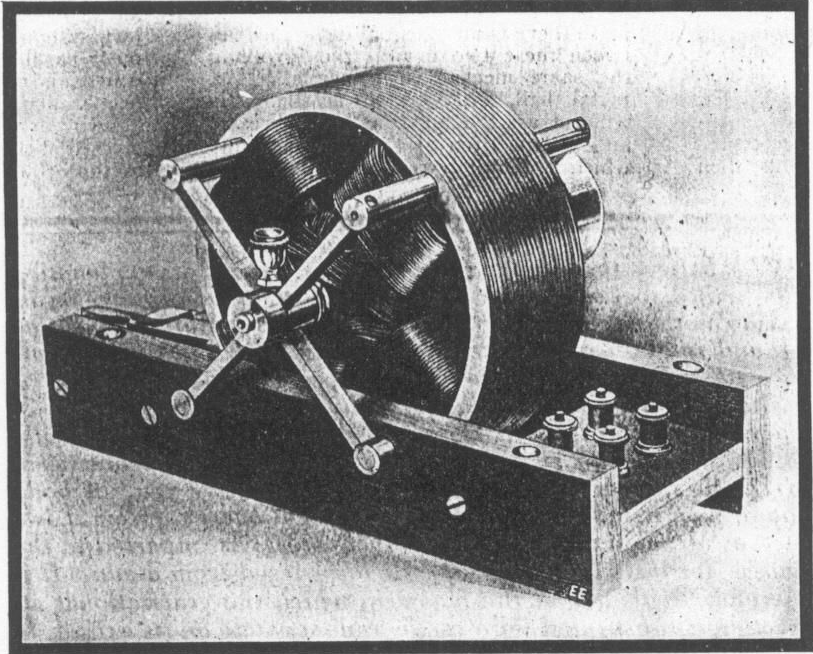
\includegraphics[width=0.63\textwidth]{IndMotor.png}
	\end{center}
	\legend{Tesla's First Induction Motor. This Historic Model is one of the two first presented before the American Institute of Electrical Engineers.}
	\vspace{-20pt}
\end{wrapfigure}
subjects and geometry;  Prof.  
Poeschl, who held the chair of theoretical and experimental physics, and Dr. Alle, who taught 
integral calculus and specialized in differential equations.  This scientist was the most brilliant 
lecturer to whom I ever listened.  He took a special interest in my progress and would frequently 
remain for an hour or two in the lecture room, giving me problems to solve, in which I delighted.  
To him I explained a flying machine I had conceived, not an illusionary invention, but one based 
on sound, scientific principles, which has become realizable thru my turbine and will soon be 
given to the world.  Both Professors Rogner and Poeschl were curious men.  The former had 
peculiar ways of expressing himself and whenever he did so there was a riot, followed by a long 
and embarrassing pause.  Prof. Poeschl was a methodical and thoroly grounded German.  He 
had enormous feet and hands like the paws of a bear, but all of his experiments were skillfully 
performed with lock-like precision and without a miss.  

It was in the second year of my studies that we received a Gramme dynamo from Paris, having 
the horseshoe form of a laminated field magnet, and a wire-wound armature with a commutator.  
It was connected up and various effects of the currents were shown.  While Prof. Poeschl was 
making demonstrations, running the machine as a motor, the brushes gave trouble, sparking 
badly, and I observed that it might be possible to operate a motor without these appliances.  But 
he declared that it could not be done and did me the honor of delivering a lecture on the subject, 
at the conclusion of which he remarked: "Mr. Tesla may accomplish great things, but he certainly 
never will do this.  It would be equivalent to converting a steadily pulling force, like that of gravity, 
into a rotary effort.  It is a perpetual motion scheme, an impossible idea." But instinct 
is something which transcends knowledge. We have, undoubtedly, certain finer fibers that enable us to 
perceive truths when logical deduction, or any other willful effort of the brain, is futile.  For a time I 
\begin{wrapfigure}{l}{0.65\textwidth}
	%	\vspace{10pt}
	\begin{minipage}[t]{.63\textwidth}
		{\centering\textsc{What is the induction motor?}\par}
		\vspace{1em}
		\itshape
		The induction motor operates on alternating current. It has no commutator like a direct current motore, nor slip rings like an alternating current motor. Contrary to the two types just cited the "field" current is not steady, but the current itself rotates constantly pulling around with it -- by induction -- the only moving part of the motor -- the rotor -- or armature. Having no armature nor slip rings, the induction motor never sparks. It consequently knows no "brush" trouble. It needs no attention because of its ruggedness. Only the bearing wear out. Its efficiency too is higher. On account of all this the induction motor is used in a prepondering proportion in street cars, electric trains, factories, etc.
	\end{minipage}
	\vspace{1em}
\end{wrapfigure}
wavered, imprest by the professor's authority, but soon became convinced I was right and 
undertook the task with all the fire and boundless confidence of youth.  

I started by first picturing in my mind a direct-current machine, running it and following the 
changing flow of the currents in the armature.  Then I would imagine an alternator and investigate 
the processes taking place in a similar manner.  Next I would visualize systems comprising 
motors and generators and operate them in various ways.  The images I saw were to me 
perfectly real and tangible.  All my remaining term in Gratz was passed in intense but fruitless 
efforts of this kind, and I almost came to the conclusion that the problem was insolvable.  

In 1880 I went to Prague, Bohemia, carrying out my father's wish to complete my education at the 
University there.  It was in that city that I made a decided advance, which consisted in detaching 
the commutator from the machine and studying the phenomena in this new aspect, but still 
without result.  In the year following there was a sudden change in my views of life.  I realized that 
my parents had been making too great sacrifices on my account and resolved to relieve them of 
the burden.  The wave of the American telephone had just reached the European continent and 
the system was to be installed in Budapest, Hungary.  It appeared an ideal opportunity, all the 
more as a friend of our family was at the head of the enterprise.  It was here that I suffered the 
complete breakdown of the nerves to which I have referred.  

What I experienced during the period of that illness surpasses all belief.  My sight and hearing 
were always extraordinary.  I could clearly discern objects in the distance when others saw no 
trace of them.  Several times in my boyhood I saved the houses of our neighbors from fire by 
hearing the faint crackling sounds which did not disturb their sleep, and calling for help.  

In 1899, when I was past forty and carrying on my experiments in Colorado, I could hear very 
distinctly thunderclaps at a distance of 550 miles.  The limit of audition for my young assistants 
was scarcely more than 150 miles.  My ear was thus over thirteen times more sensitive.  Yet at 
that time I was, so to speak, stone deaf in comparison with the acuteness of my hearing while 
under the nervous strain.  In Budapest I could hear the ticking of a watch with three rooms 
between me and the time-piece.  A fly alighting on a table in the room would cause a dull thud in 
my ear.  A carriage passing at a distance of a few miles fairly shook my whole body.  The whistle 
of a locomotive twenty or thirty miles away made the bench or chair on which I sat vibrate so 
strongly that the pain was unbearable.  The ground under my feet trembled continuously.  I had to 
support my bed on rubber cushions to get any rest at all.  The roaring noises from near and far 
often produced the effect of spoken words which would have frightened me had I not been able to 
resolve them into their accidental components.  The sun's rays, when periodically intercepted, 
would cause blows of such force on my brain that they would stun me.  I had to summon all my 
will power to pass under a bridge or other structure as I experienced a crushing pressure on the 
skull.  In the dark I had the sense of a bat and could detect the presence of an object at a 
distance of twelve feet by a peculiar creepy sensation on the forehead.  My pulse varied from a 
few to two hundred and sixty beats and all the tissues of the body quivered with twitchings and 
tremors which was perhaps the hardest to bear.  A renowned physician who gave me daily large 
doses of Bromide of Potassium pronounced my malady unique and incurable.  

It is my eternal regret that I was not under the observation of experts in physiology and 
psychology at that time.  I clung desperately to life, but never expected to recover.  Can anyone 
believe that so hopeless a physical wreck could ever be transformed into a man of astonishing 
strength and tenacity, able to work thirty-eight years almost without a day's interruption, and find 
himself still strong and fresh in body and mind? Such is my case.  A powerful desire to live and to 
continue the work, and the assistance of a devoted friend and athlete accomplished the wonder.  
My health returned and with it the vigor of mind.  In attacking the problem again I almost regretted 
that the struggle was soon to end.  I had so much energy to spare.  When I undertook the task it 
was not with a resolve such as men often make.  With me it was a sacred vow, a question of life 
and death.  I knew that I would perish if I failed.  Now I felt that the battle was won.  Back in the 
deep recesses of the brain was the solution, but I could not yet give it outward expression.  One 
afternoon, which is ever present in my recollection, I was enjoying a walk with my friend in the 
City Park and reciting poetry.  At that age I knew entire books by heart, word for word.  One of 
these was Goethe's "Faust." The sun was just setting and reminded me of the glorious passage:
\begin{verse}
"Sie ruckt und weicht, der Tag ist uberlebt,\\ 
Dort eilt sie hin und fordert neues Leben.\\
Oh, dass kein Flugel mich vom Boden hebt\\
Ihr nach und immer nach zu streben!\\
\vspace{1em}
Ein schoner Traum indessen sie entweicht,\\
Ach, zu des Geistes Flugeln wird so leicht\\
Kein korperlicher Flugel sich gesellen!"
\footnote{\vspace{-2em}
	\begin{verse}
		The glow retreats, done is the day of toil;\\
		It yonder hastes, new fields of life exploring;\\
		Ah, that no wing can lift me from the soil\\
		Upon its track to follow, follow soaring!\\
		\vspace{1em}
		A glorious dream! though now the glories fade.\\
		Alas! the wings that lift the mind no aid\\
		Of wings to lift the body can bequeath me.
	\end{verse}
}		
\end{verse}


As I uttered these inspiring words the idea came like a flash of lightning and in an instant the truth 
was revealed.  I drew with a stick on the sand the diagrams shown six years later in my address 
before the American Institute of Electrical Engineers, and my companion understood them 
perfectly.  The images I saw were wonderfully sharp and clear and had the solidity of metal and 
stone, so much so that I told him: "See my motor here; watch me reverse it." I cannot begin to 
describe my emotions.  Pygmalion seeing his statue come to life could not have been more 
deeply moved.  A thousand secrets of nature which I might have stumbled upon accidentally I 
would have given for that one which I had wrested from her against all odds and at the peril of my 
existence.
\newpage 


	\vspace*{\stretch{1}}
	{\centering
		\aldine\\
		\aldine\hspace{1.2em}\aldine
		\par}
	\vspace*{2cm}
	


%%------------------Chapitre 4 ------------------
\cleardoublepage
\thispagestyle{empty}
\markboth{The Discovery of the Tesla Coil and Transformer}{}
\vspace*{5em}
\begin{center}
	\bfseries
	\noindent {\Large\decofourleft~\textsc{IV}~\decofourright}\\
	\noindent\rule{.5\linewidth}{1pt}\\
	\medskip
	{\noindent\LARGE The Discovery of the\\Tesla Coil and Transformer}
	
	\bigskip
	{\normalfont\smallskip\footnotesize\protect\parbox{.75\linewidth}{\itshape
			\lettrine[lines=2]{T}{he} proverbial trials and tribulations known to every inventor were not spared Tesla, the world's greatest inventor of all times. In this article we see him, arrived at young manhood, struggling along in cold world. Already his fame has spread far and wide and his genius is recognized. But converting genius and fame into dollars and cents is quite a different matter, and the world is full of unappreciative and unscrupulous men. Tesla, the idealist, cared little for money and thus was promptly taken advantage of. But let Tesla himself tell you in his own inimitable style. It is a wonderful story.
			
			In this month's installment Tesla also tells us how he made one of his most important as well as sensational discoveries--the Tesla Coil. Few inventions have caused such a sensation as this one which culminated in the only man-made lightning ever produced. The Tesla coil has so many uses and has been built in so many styles that it would take a catalog to list them all . From the spectacular high frequency stunts on the stage down to the "violet`` ray machine in your home; all are Tesla coils in one form or another.
			
			Wireless without the Tesla Coil would not be possible today. Without an oscillation transformer, spark gap and condenser --which is a Tesla Coil-- the sending station would be crippled.
			
			But it is for industrial purposes where the Tesla Coil will shine brightest in the future. The production of Ozone, the extraction of Nitrogen from the air in huge quantities--all are children of Tesla's fertile breain. His coil is the key to them all.\\
			
			\hfill --\scshape{Editor}.
		}
		\par
	}
	\vspace*{5em}
\end{center}

\addtocontents{toc}{\normalsize}
\addcontentsline{toc}{section}{The Discovery of the Tesla Coil and Transformer}




For a while I gave myself up entirely to the intense enjoyment of picturing machines and devising 
new forms.  It was a mental state of happiness about as complete as I have ever known in life.  
Ideas came in an uninterrupted stream and the only difficulty I had was to hold them fast.  The 
pieces of apparatus I conceived were to me absolutely real and tangible in every detail, even to 
the minute marks and signs of wear.  I delighted in imagining the motors constantly running, for in 
this way they presented to mind's eye a more fascinating sight.  When natural inclination 
develops into a passionate desire, one advances towards his goal in seven-league boots.  In less 
than two months I evolved virtually all the types of motors and modifications of the system which 
are now identified with my name.  It was, perhaps, providential that the necessities of existence 
commanded a temporary halt to this consuming activity of the mind.  I came to Budapest 
prompted by a premature report concerning the telephone enterprise and, as irony of fate willed 
it, I had to accept a position as draftsman in the Central Telegraph Office of the Hungarian 
Government at a salary which I deem it my privilege not to disclose! Fortunately, I soon won the 
interest of the Inspector-in-Chief and was thereafter employed on calculations, designs and 
estimates in connection with new installations, until the Telephone Exchange was started, when I 
took charge of the same.  The knowledge and practical experience I gained in the course of this 
work was most valuable and the employment gave me ample opportunities for the exercise of my 
inventive faculties.  I made several improvements in the Central Station apparatus and perfected 
a telephone repeater or amplifier which was never patented or publicly described but would be 
creditable to me even today.  In recognition of my efficient assistance the organizer of the 
undertaking, Mr. Puskas, upon disposing of his business in Budapest, offered me a position in 
Paris which I gladly accepted.  

I never can forget the deep impression that magic city produced on my mind.  For several days 
after my arrival I roamed thru the streets in utter bewilderment of the new spectacle.  The 
attractions were many and irresistible, but, alas, the income was spent as soon as received.  
When Mr. Puskas asked me how I was getting along in the new sphere, I described the situation 
accurately in the statement that "the last twenty-nine days of the month are the toughest!" I led a 
rather strenuous life in what would now be termed "Rooseveltian fashion." Every morning, 
regardless of weather, I would go from the Boulevard St.  Marcel, where I resided, to a bathing 
house on the Seine, plunge into the water, loop the circuit twenty-seven times and then walk an 
hour to reach Ivry, where the Company's factory was located.  There I would have a 
woodchopper's breakfast at half-past seven o'clock and then eagerly await the lunch hour, in the 
meanwhile cracking hard nuts for the Manager of the Works, Mr. Charles Batchellor, who was an 
intimate friend and assistant of Edison.  Here I was thrown in contact with a few Americans who 
fairly fell in love with me because of my proficiency in billiards.  To these men I explained my 
invention and one of them, Mr. D. Cunningham, Foreman of the Mechanical Department, offered 
to form a stock company.  The proposal seemed to me comical in the extreme.  I did not have the 
faintest conception of what that meant except that it was an American way of doing things.  
Nothing came of it, however, and during the next
\begin{wrapfigure}{r}{0.65\textwidth}
	\vspace{-20pt}
	\begin{center}
		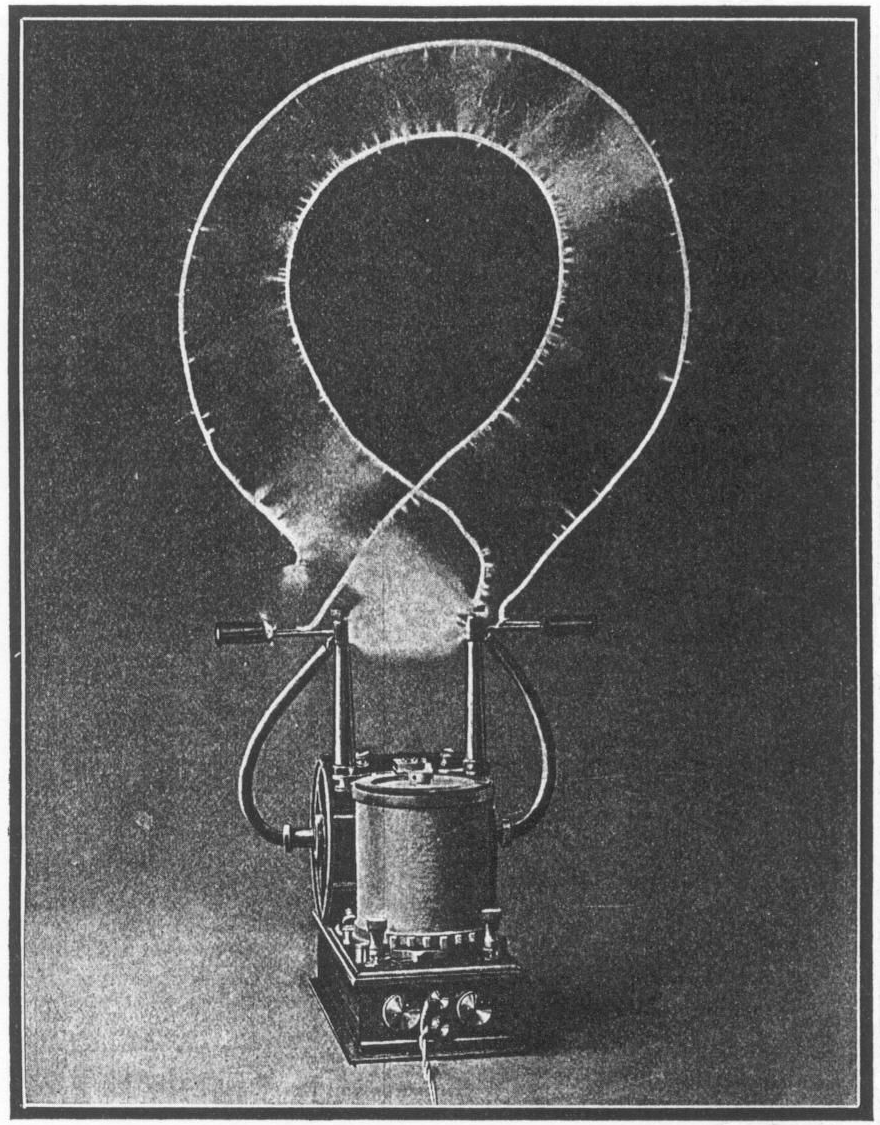
\includegraphics[width=0.63\textwidth]{OscillationTransformer.png}
	\end{center}
	\legend{Tesla Oscillation Transformer (Tesla Coil) Presented by Lord Kelvin Before the British Association In August, 1897. This Small and Compact Instrument, Only 8 Inches High, Developed Two Square Feet of Streamers With Twenty-Five Watts from the $110$ Volts D.C. Supply Circuit. The Instrument Contains a Tesla Primary and Secondary, Condenser, and a Circuit Controller.}
	\vspace{-20pt}
\end{wrapfigure}
 few months I had to travel from one to another 
place in France and Germany to cure the ills of the power plants.  On my return to Paris I 
submitted to one of the administrators of the Company, Mr. Rau, a plan for improving their 
dynamos and was given an opportunity.  My success was complete and the delighted directors accorded me the privilege of developing automatic regulators which were much desired.  Shortly 
after there was some trouble with the lighting plant which had been installed at the new railroad 
station in Strassburg, Alsace.  The wiring was defective and on the occasion of the opening 
ceremonies a large part of a wall was blown out thru a short-circuit right in the presence of old 
Emperor William I.  The German Government refused to take the plant and the French Company 
was facing a serious loss.  On account of my knowledge of the German language and past 
experience, I was entrusted with the difficult task of straightening out matters and early in 1883 I 
went to Strassburg on that mission.  

\vspace{-1em}
\subsection{The First Induction Motor is Built}

Some of the incidents in that city have left an indelible record on my memory.  By a curious 
coincidence, a number of men who subsequently achieved fame, lived there about that time.  In 
later life I used to say, "There were bacteria of greatness in that old town.  Others caught the 
disease but I escaped!" The practical work, correspondence, and conferences with officials kept 
me preoccupied day and night, but, as soon as I was able to manage I undertook the construction 
of a simple motor in a mechanical shop opposite the railroad station, having brought with me from 
Paris some material for that purpose.  The consummation of the experiment was, however, 
delayed until the summer of that year when I finally had the satisfaction of seeing rotation effected 
by alternating currents of different phase, and without sliding contacts or commutator, as I had 
conceived a year before.  It was an exquisite pleasure but not to compare with the delirium of joy 
following the first revelation.  

Among my new friends was the former Mayor of the city, Mr. Bauzin, whom I had already in a 
measure acquainted with this and other inventions of mine and whose support I endeavored to 
enlist.  He was sincerely devoted to me and put my project before several wealthy persons but, to 
my mortification, found no response.  He wanted to help me in every possible way and the 
approach of the first of July, 1919, happens to remind me of a form of "assistance" I received 
from that charming man, which was not financial but none the less appreciated.  In 1870, when 
the Germans invaded the country, Mr. Bauzin had buried a good sized allotment of St. Estephe of 
1801 and he came to the conclusion that he knew no worthier person than myself to consume 
that precious beverage.  This, I may say, is one of the unforgettable incidents to which I have 
referred.  My friend urged me to return to Paris as soon as possible and seek support there.  This 
I was anxious to do but my work and negotiations were protracted owing to all sorts of petty 
obstacles I encountered so that at times the situation seemed hopeless.  

\subsection{German ``Efficiency"}
Just to give an idea of German thoroness and "efficiency," I may mention here a rather funny 
experience.  An incandescent lamp of 16 c.p.  was to be placed in a hallway and upon selecting 
the proper location I ordered the monteur to run the wires.  After working for a while he concluded 
that the engineer had to be consulted and this was done.  The latter made several objections but 
ultimately agreed that the lamp should be placed two inches from the spot I had assigned, 
whereupon the work proceeded.  Then the engineer became worried and told me that Inspector 
Averdeck should be notified.  That important person called, investigated, debated, and decided 
that the lamp should be shifted back two inches, which was the place I had marked.  It was not 
long, however, before Averdeck got cold feet himself and advised me that he had informed Ober-
Inspector Hieronimus of the matter and that I should await his decision.  It was several days 
before the Ober-Inspector was able to free himself of other pressing duties but at last he arrived 
and a two-hour debate followed, when he decided to move the lamp two inches farther.  My hopes that this was the 
\begin{wrapfigure}{r}{0.65\textwidth}
	\vspace{-20pt}
	\begin{center}
		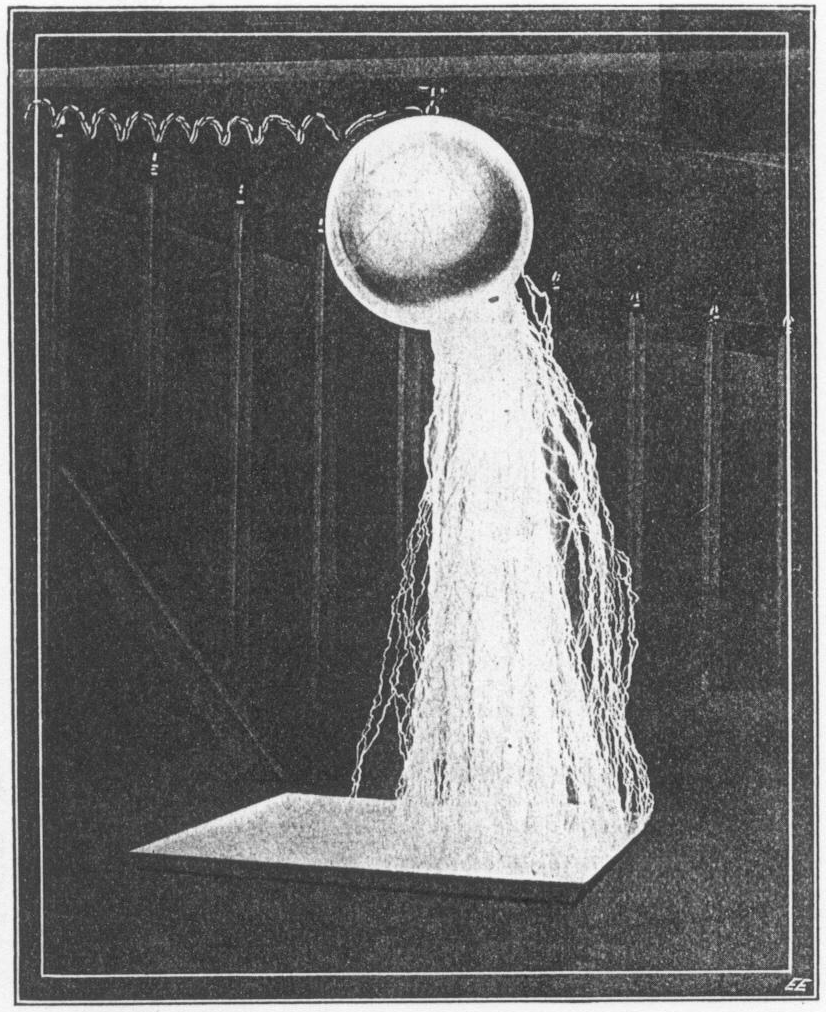
\includegraphics[width=0.63\textwidth]{Sparks.png}
	\end{center}
	\legend{This Illustrates Tests with Spark Discharges from a Ball of Forty Centimeters Radius in Tesla's Wireless Plant Erected at Colorado Springs in 1899. The Ball is Connected to the Free End of a Grounded Resonant Circuit Seventeen Meters in Diameter. The Disruptive Potential of a Ball, is, according to Tesla, in Volts Approximatelly $V=75,400\ r$ ($r$ being in Centimeters), that is, in this Case $75,400\times 40=3,016,000\ Volts$. The Gigantic Tesla Coil which Produced these Bolts of Thor was Capable of Furnishing a Current of $1,100$ Amperes in the High Tension Secondary. The Primary Coil had a Diameter of $51$ Feet! This Tesla Coil Produced Discharges which were the Nearest Approach to Lightning Ever Made by Man.}
	\vspace{-20pt}
\end{wrapfigure}
final act were shattered when the Ober-Inspector returned and said to 
me: "Regierungsrath Funke is so particular that I would not dare to give an order for placing this 
lamp without his explicit approval." Accordingly arrangements for a visit from that great man were 
made.  We started cleaning up and polishing early in the morning.  Everybody brushed up, I put 
on my gloves and when Funke came with his retinue he was ceremoniously received.  After two 
hours' deliberation he suddenly exclaimed: "I must be going," and pointing to a place on the 
ceiling, he ordered me to put the lamp there.  It was the exact spot which I had originally chosen, 

So it went day after day with variations, but I was determined to achieve at whatever cost and in 
the end my efforts were rewarded.  By the spring of 1884 all the differences were adjusted, the 
plant formally accepted, and I returned to Paris with pleasing anticipations.  One of the 
administrators had promised me a liberal compensation in case I succeeded, as well as a fair 
consideration of the improvements I had made in their dynamos and I hoped to realize a 
substantial sum.  There were three administrators whom I shall designate as A, B and C for 
convenience.  When I called on A he told me that B had the say.  This gentleman thought that 
only C could decide and the latter was quite sure that A alone had the power to act.  After several 
laps of this circulus vivios it dawned upon me that my reward was a castle in Spain.  The utter 
failure of my attempts to raise capital for development was another disappointment
and when Mr. 
Batchellor prest me to go to America with a view of redesigning the Edison machines, I 
determined to try my fortunes in the Land of Golden Promise.  But the chance was nearly mist.  I 
liquefied my modest assets, secured accommodations and found myself at the railroad station as 
the train was pulling out.  At that moment I discovered that my money and tickets were gone.  
What to do was the question.  Hercules had plenty of time to deliberate but I had to decide while 
running alongside the train with opposite feelings surging in my brain like condenser oscillations.  
Resolve, helped by dexterity, won out in the nick of time and upon passing thru the usual 
experiences, as trivial as unpleasant, I managed to embark for New York with the remnants of my 
belongings, some poems and articles I had written, and a package of calculations relating to 
solutions of an unsolvable integral and to my flying machine.  During the voyage I sat most of the 
time at the stern of the ship watching for an opportunity to save somebody from a watery grave, 
without the slightest thought of danger.  Later when I had absorbed some of the practical 
American sense I shivered at the recollection and marvelled at my former folly.  

\vspace{-1em}
\subsection{Tesla in America}
I wish that I could put in words my first impressions of this country.  In the Arabian Tales I read 
how genii transported people into a land of dreams to live thru delightful adventures.  My case 
was just the reverse.  The genii had carried me from a world of dreams into one of realities.  What 
I had left was beautiful, artistic and fascinating in every way; what I saw here was machined, 
rough and unattractive.  A burly policeman was twirling his stick which looked to me as big as a 
log.  I approached him politely with the request to direct me.  "Six blocks down, then to the left," 
he said, with murder in his eyes.  "Is this America?" I asked myself in painful surprise.  "It is a 
century behind Europe in civilization." When I went abroad in 1889 - five years having elapsed 
since my arrival here - I became convinced that it was more than one hundred years AHEAD of 
Europe and nothing has happened to this day to change my opinion.  

\vspace{-1em}
\subsection{Tesla Meets Edison}
The meeting with Edison was a memorable event in my life.  I was amazed at this wonderful man 
who, without early advantages and scientific training, had accomplished so much.  I had studied a 
dozen languages, delved in literature and art, and had spent my best years in libraries reading all 
sorts of stuff that fell into my hands, from Newton's "Principia" to the novels of Paul de Kock, and 
felt that most of my life had been squandered.  But it did not take long before I recognized that it 
was the best thing I could have done.  Within a few weeks I had won Edison's confidence and it 
came about in this way.  

The S.S. Oregon, the fastest passenger steamer at that time, had both of its lighting machines 
disabled and its sailing was delayed.  As the superstructure had been built after their installation it 
was impossible to remove them from the hold.  The predicament was a serious one and Edison 
was much annoyed.  In the evening I took the necessary instruments with me and went aboard 
the vessel where I stayed for the night.  The dynamos were in bad condition, having several 
short-circuits and breaks, but with the assistance of the crew I succeeded in putting them in good 
shape.  At five o'clock in the morning, when passing along Fifth Avenue on my way to the shop, I 
met Edison with Batchellor and a few others as they were returning home to retire.  "Here is our 
Parisian running around at night," he said.  When I told him that I was coming from the Oregon 
and had repaired both machines, he looked at me in silence and walked away without another 
word.  But when he had gone some distance I heard him remark: "Batchellor, this is a d-n good 
man," and from that time on I had full freedom in directing the work.  For nearly a year my regular 
hours were from 10.30 A.M.  until 5 o'clock the next morning without a day's exception.  Edison 
said to me: "I have had many hard-working assistants but you take the cake." During this period I 
designed twenty-four different types of standard machines with short cores and of uniform pattern 
which replaced the old ones.  The Manager had promised me fifty thousand dollars on the completion of this  task but it turned out to be a practical joke.  This gave me a painful shock and I resigned my position.  


Immediately thereafter some people approached me with the proposal of forming an arc light 
company under my name, to which I agreed.  Here finally was an opportunity to develop the 
motor, but when I broached the subject to my new associates they said: "No, we want the arc 
lamp.  We don't care for this alternating current of yours." In 1886 my system of arc lighting was 
perfected and adopted for factory and municipal lighting, and I was free, but with no other 
possession than a beautifully engraved certificate of stock of hypothetical value.  Then followed a 
period of struggle in the new medium for which I was not fitted, but the reward came in the end 
and in April, 1887, the Tesla Electric Company was organized, providing a laboratory and 
facilities.  The motors I built there were exactly as I had imagined them.  I made no attempt to 
improve the design, but merely reproduced the pictures as they appeared to my vision and the 
operation was always as I expected.  

In the early part of 1888 an arrangement was made with the Westinghouse Company for the 
manufacture of the motors on a large scale.  But great difficulties had still to be overcome.  My 
system was based on the use of low frequency currents and the Westinghouse experts had 
adopted 133 cycles with the object of securing advantages in the transformation.  They did not 
want to depart from their standard forms of apparatus and my efforts had to be concentrated 
upon adapting the motor to these conditions.  Another necessity was to produce a motor capable 
of running efficiently at this frequency on two wires which was not easy of accomplishment.  



At the close of 1889, however, my services in Pittsburg being no longer essential, I returned to 
New York and resumed experimental work in a laboratory on Grand Street, where I began 
immediately the design of high frequency machines.  The problems of construction in this 
unexplored field were novel and quite peculiar and I encountered many difficulties.  I rejected the 
inductor type, fearing that it might not yield perfect sine waves which were so important to 
resonant action.  Had it not been for this I could have saved myself a great deal of labor.  Another 
discouraging feature of the high frequency alternator seemed to be the inconstancy of speed 
which threatened to impose serious limitations to its use.  I had already noted in my 
demonstrations before the American Institution of Electrical Engineers that several times the tune 
was lost, necessitating readjustment, and did not yet foresee, what I discovered long afterwards, 
a means of operating a machine of this kind at a speed constant to such a degree as not to vary 
more than a small fraction of one revolution between the extremes of load.  


\begin{figure}[p]
	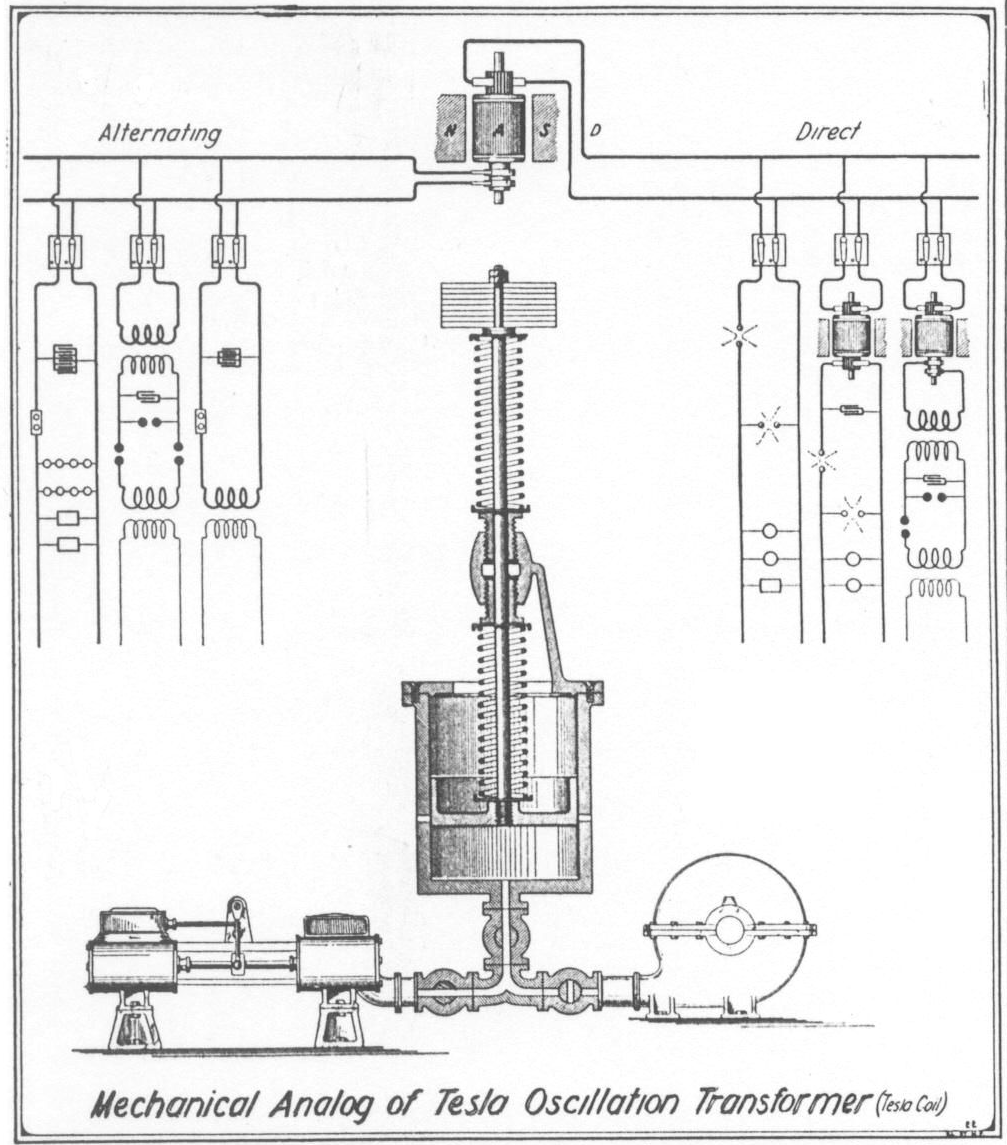
\includegraphics[width=\textwidth]{MechA.png}
	\legend{Tesla Oscillation Transformer (Tesla Coil) Presented by Lord Kelvin Before the British Association In August, 1897. This small and compact instrument, only 8 inches high, developed two square feet of streamers with twenty-five watts from the 110 volts D.C. Supply Circuit. The Instrument contains a Tesla Primary and Secondary, Condenser, and a Circuit Controller.}
\end{figure}


\subsection{The Invention of the Tesla Coil}
From many other considerations it appeared desirable to invent a simpler device for the 
production of electric oscillations.  In 1856 Lord Kelvin had exposed the theory of the condenser 
discharge, but no practical application of that important knowledge was made.  I saw the 
possibilities and undertook the development of induction apparatus on this principle.  My progress 
was so rapid as to enable me to exhibit at my lecture in 1891 a coil giving sparks of five inches.  
On that occasion I frankly told the engineers of a defect involved in the transformation by the new 
method, namely, the loss in the spark gap.  Subsequent investigation showed that no matter what 
medium is employed, be it air, hydrogen, mercury vapor, oil or a stream of electrons, the 
efficiency is the same.  It is a law very much like that governing the conversion of mechanical 
energy.  We may drop a weight from a certain height vertically down or carry it to the lower level 
along any devious path, it is immaterial insofar as the amount of work is concerned.  Fortunately 
however, this drawback is not fatal as by proper proportioning of the resonant circuits an 
efficiency of 85 per cent is attainable.  Since my early announcement of the invention it has come 
into universal use and wrought a revolution in many departments.  But a still greater future awaits 
it.  When in 1900 I obtained powerful discharges of 100 feet and flashed a current around the 
globe, I was reminded of the first tiny spark I observed in my Grand Street laboratory and was 
thrilled by sensations akin to those I felt when I discovered the rotating magnetic field.  



	\vspace*{\stretch{1}}
	{\centering
		\aldine\\
		\aldine\hspace{1.2em}\aldine
		\par}
	\vspace*{2cm}
	


%%------------------Chapitre 5 ------------------
\cleardoublepage
\thispagestyle{empty}
\markboth{The Magnifying Transmitter}{}
\vspace*{5em}
\begin{center}
	\bfseries
	\noindent {\Large\decofourleft~\textsc{V}~\decofourright}\\
	\noindent\rule{.5\linewidth}{1pt}\\
	\medskip
	{\noindent\LARGE The Magnifying\\Transmitter}
	
	\bigskip
	
	{\normalfont\smallskip\footnotesize\protect\parbox{.75\linewidth}{\itshape
			\lettrine[lines=2]{I}{magine} a man a century ago, bold enough to design and actually build a huge tower with which to transmit the human voice, music, pictures, press news and even power, thru the earth to any distance whatever without wires! He probably would have been hung or burnt at the stake. So when Tesla built his famous tower on Long Island he was a hundred years ahead of his time. And foolish ridicule by our latter day arm-chair ``savants", does not in the least mar Tesla's greatness.
			
			The titanic brain of Tesla has hardly produced a more amazing wonder than this ``magnifying transmitter". Contrary to popular belief his tower was not built to radiate Hertzian waves into the ether. Tesla's system sends out thousands of horsepower thru the earth -- he has shown experimentally how power can be sent without wires over distances from a central point. Nor is there any mystery about it how he accomplishes the result. His historic U.S. patents and articles describe the method used. Tesla's Magnifying Transmitter is truly a modern lamp of Aladdin.	\\
			
			\hfill --\scshape{Editor}.
		}
		\par
	}
	\vspace*{5em}
\end{center}

\addtocontents{toc}{\normalsize}
\addcontentsline{toc}{section}{The Magnifying Transmitter}


As I review the events of my past life I realize how subtle are the influences that shape our 
destinies.  An incident of my youth may serve to illustrate.  One winter's day I managed to climb a 
steep mountain, in company with other boys.  The snow was quite deep and a warm southerly 
wind made it just suitable for our purpose.  We amused ourselves by throwing balls which would 
roll down a certain distance, gathering more or less snow, and we tried to outdo one another in 
this exciting sport.  Suddenly a ball was seen to go beyond the limit, swelling to enormous 
proportions until it became as big as a house and plunged thundering into the valley below with a 
force that made the ground tremble.  I looked on spellbound, incapable of understanding what 
had happened.  For weeks afterward the picture of the avalanche was before my eyes and I 
wondered how anything so small could grow to such an immense size.  Ever since that time the 
magnification of feeble actions fascinated me, and when, years later, I took up the experimental 
study of mechanical and electrical resonance, I was keenly interested from the very start.  
Possibly, had it not been for that early powerful impression, I might not have followed up the little 
spark I obtained with my coil and never developed my best invention, the true history of which I'll 
tell here for the first time.  

\subsection{Scrapping The World's Engines}
"Lionhunters" have often asked me which of my discoveries I prize most.  This depends on the 
point of view.  Not a few technical men, very able in their special departments, but dominated by 
a pedantic spirit and nearsighted, have asserted that excepting the induction motor I have given 
to the world little of practical use.  This is a grievous mistake.  A new idea must not be judged by 
its immediate results.  My alternating system of power transmission came at a psychological 
moment, as a long-sought answer to pressing industrial questions, and altho considerable 
resistance had to be overcome and opposing interests reconciled, as usual, the commercial 
introduction could not be long delayed.  Now, compare this situation with that confronting my 
turbine, for example.  One should think that so simple and beautiful an invention, possessing 
many features of an ideal motor, should be adopted at once and, undoubtedly, it would under 
similar conditions.  But the prospective effect of the rotating field was not to render worthless 
existing machinery; on the contrary, it was to give it additional value.  The system lent itself to 
new enterprise as well as to improvement of the old.  My turbine is an advance of a character 
entirely different.  It is a radical departure in the sense that its success would mean the 
abandonment of the antiquated types of prime movers on which billions of dollars have been 
spent.  Under such circumstances the progress must needs be slow and perhaps the greatest 
impediment is encountered in the prejudicial opinions created in the minds of experts by 
organized opposition.  

Only the other day I had a disheartening experience when I met my friend and former assistant, 
Charles F. Scott, now professor of Electrical Engineering at Yale.  I had not seen him for a long 
time and was glad to have an opportunity for a little chat at my office.  Our conversation naturally 
enough drifted on my turbine and I became heated to a high degree.  "Scott," I exclaimed, carried 
away by the vision of a glorious future, "my turbine will scrap all the heat-engines in the world." 
Scott stroked his chin and looked away thoughtfully, as though making a mental calculation.  
"That will make quite a pile of scrap," he said, and left without another word! 
\begin{figure}[p]
	\vspace*{\stretch{1}}
	\begin{center}
		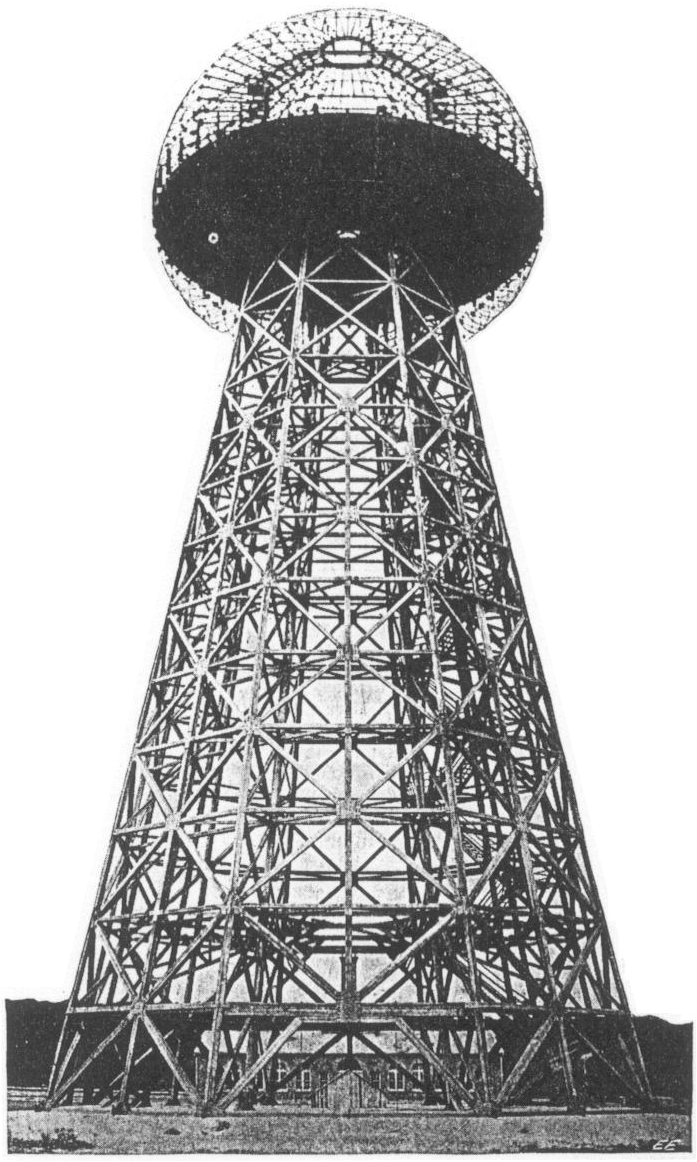
\includegraphics[height=.75\textheight]{Tower.png}
	\end{center}
	\legend{This photograph shows the famous Tesla Tower erected at Shoreham, L. I.,N. Y. The Tower was dismantled at the outbreak of the war. It was 187 feet high. The spherical top was 68 feet in diameter. Note the huge size of the structure by comparing the two-story power plant in the rear. The Tower which was to be used by Tesla in hs ``World Wireless", was never finished. Next illustration shows it completed}
	\vspace*{\stretch{1}}
\end{figure}

\subsection{``Aladdin's Lamp"}
These and other inventions of mine, however, were nothing more than steps forward in certain 
directions.  In evolving them I simply followed the inborn sense to improve the present devices 
without any special thought of our far more imperative necessities.  The "Magnifying Transmitter" 
was the product of labors extending through years, having for their chief object the solution of 
problems which are infinitely more important to mankind than mere industrial development.If my memory serves me right, it was in November, 1890, that I performed a laboratory 
experiment which was one of the most extraordinary and spectacular ever recorded in the annals 
of science.  In investigating the behaviour of high frequency currents I had satisfied myself that an 
electric field of sufficient intensity could be produced in a room to light up electrodeless vacuum 
tubes.  Accordingly, a transformer was built to test the theory and the first trial proved a 
marvelous success.  It is difficult to appreciate what those strange phenomena meant at that time.  
We crave for new sensations but soon become indifferent to them.  The wonders of yesterday are 
today common occurrences.  When my tubes were first publicly exhibited they were viewed with 
amazement impossible to describe.  From all parts of the world I received urgent invitations and 
numerous honors and other flattering inducements were offered to me, which I declined.  


\subsection{In Faraday's Chair}
But in 1892 the demands became irresistible and I went to London where I delivered a lecture 
before the Institution of Electrical Engineers.  It had been my intention to leave immediately for 
Paris in compliance with a similar obligation, but Sir James Dewar insisted on my appearing 
before the Royal Institution.  I was a man of firm resolve but succumbed easily to the forceful 
arguments of the great Scotsman.  He pushed me into a chair and poured out half a glass of a 
wonderful brown fluid which sparkled in all sorts of iridescent colors and tasted like nectar.  
"Now," said he.  "you are sitting in Faraday's chair and you are enjoying whiskey he used to 
drink." In both aspects it was an enviable experience.  The next evening I gave a demonstration 
before that Institution, at the termination of which Lord Rayleigh addressed the audience and his 
generous words gave me the first start in these endeavors.  I fled from London and later from 
Paris to escape favors showered upon me, and journeyed to my home where I passed through a 
most painful ordeal and illness.  Upon regaining my health I began to formulate plans for the 
resumption of work in America.  Up to that time I never realized that I possessed any particular 
gift of discovery but Lord Rayleigh, whom I always considered as an ideal man of science, had 
said so and if that was the case I felt that I should concentrate on some big idea.  

\subsection{Nature's Trigger}
One day, as I was roaming in the mountains, I sought shelter from an approaching storm.  The 
sky became overhung with heavy clouds but somehow the rain was delayed until, all of a sudden, 
there was a lightning flash and a few moments after a deluge.  This observation set me thinking.  
It was manifest that the two phenomena were closely related, as cause and effect, and a little 
reflection led me to the conclusion that the electrical energy involved in the precipitation of the 
water was inconsiderable, the function of lightning being much like that of a sensitive trigger.  

Here was a stupendous possibility of achievement.  If we could produce electric effects of the 
required quality, this whole planet and the conditions of existence on it could be transformed.  
The sun raises the water of the oceans and winds drive it to distant regions where it remains in a 
state of most delicate balance.  If it were in our power to upset it when and wherever desired, this 
mighty life-sustaining stream could be at will controlled.  We could irrigate arid deserts, create 
lakes and rivers and provide motive power in unlimited amounts.  This would be the most efficient 
way of harnessing the sun to the uses of man.  The consummation depended on our ability to 
develop electric forces of the order of those in nature.  It seemed a hopeless undertaking, but I 
made up my mind to try it and immediately on my return to the United States, in the Summer of 
1892, work was begun which was to me all the more attractive, because a means of the same 
kind was necessary for the successful transmission of energy without wires.  

\subsection{Four Million Volts}
The first gratifying result was obtained in the spring of the succeeding year when I reached 
tensions of about 1,000,000 volts with my conical coil.  That was not much in the light of the 
present art, but it was then considered a feat.  Steady progress was made until the destruction of 
my laboratory by fire in 1895, as may be judged from an article by T. C. Martin which appeared in 
the April number of the Century Magazine.  This calamity set me back in many ways and most of 
that year had to be devoted to planning and reconstruction.  However, as soon as circumstances 
permitted, I returned to the task.  

Although I knew that higher electro-motive forces were attainable with apparatus of larger 
dimensions, I had an instinctive perception that the object could be accomplished by the proper 
design of a comparatively small and compact transformer.  In carrying on tests with a secondary 
in the form of a flat spiral, as illustrated in my patents, the absence of streamers surprised me, 
and it was not long before I discovered that this was due to the position of the turns and their 
mutual action.  Profiting from this observation I resorted to the use of a high tension conductor 
with turns of considerable diameter sufficiently separated to keep down the distributed capacity, 
while at the same time preventing undue accumulation of the charge at any point.  The 
application of this principle enabled me to produce pressures of 4,000,000 volts, which was about 
the limit obtainable in my new laboratory at Houston Street, as the discharges extended through a 
distance of 16 feet.  A photograph of this transmitter was published in the Electrical Review of 
November, 1898.  

In order to advance further along this line I had to go into the open, and in the spring of 1899, 
having completed preparations for the erection of a wireless plant, I went to Colorado where I 
remained for more than one year.  Here I introduced other improvements and refinements which 
made it possible to generate currents of any tension that may be desired.  Those who are 
interested will find some information in regard to the experiments I conducted there in my article, 
"The Problem of Increasing Human Energy" in the Century Magazine of June, 1900, to which I 
have referred on a previous occasion.  

\subsection{The Magnifying Transmitter}
I have been asked by the \textsc{Electrical Experimenter} to be quite explicit on this subject so 
that my young friends among the readers of the magazine will clearly understand the construction 
and operation of my "Magnifying Transmitter" and the purposes for which it is intended.  Well, 
then, in the first place, it is a resonant transformer with a secondary in which the parts, charged to 
a high potential, are of considerable area and arranged in space along ideal enveloping surfaces 
of very large radii of curvature, and at proper distances from one another thereby insuring a small 
electric surface density everywhere so that no leak can occur even if the conductor is bare.  It is 
suitable for any frequency, from a few to many thousands of cycles per second, and can be used 
in the production of currents of tremendous volume and moderate pressure, or of smaller 
amperage and immense electromotive force.  The maximum electric tension is merely dependent 
on the curvature of the surfaces on which the charged elements are situated and the area of the 
latter.  

\begin{figure}[p]
	\vspace*{-2cm}
	\makebox[\linewidth]{
		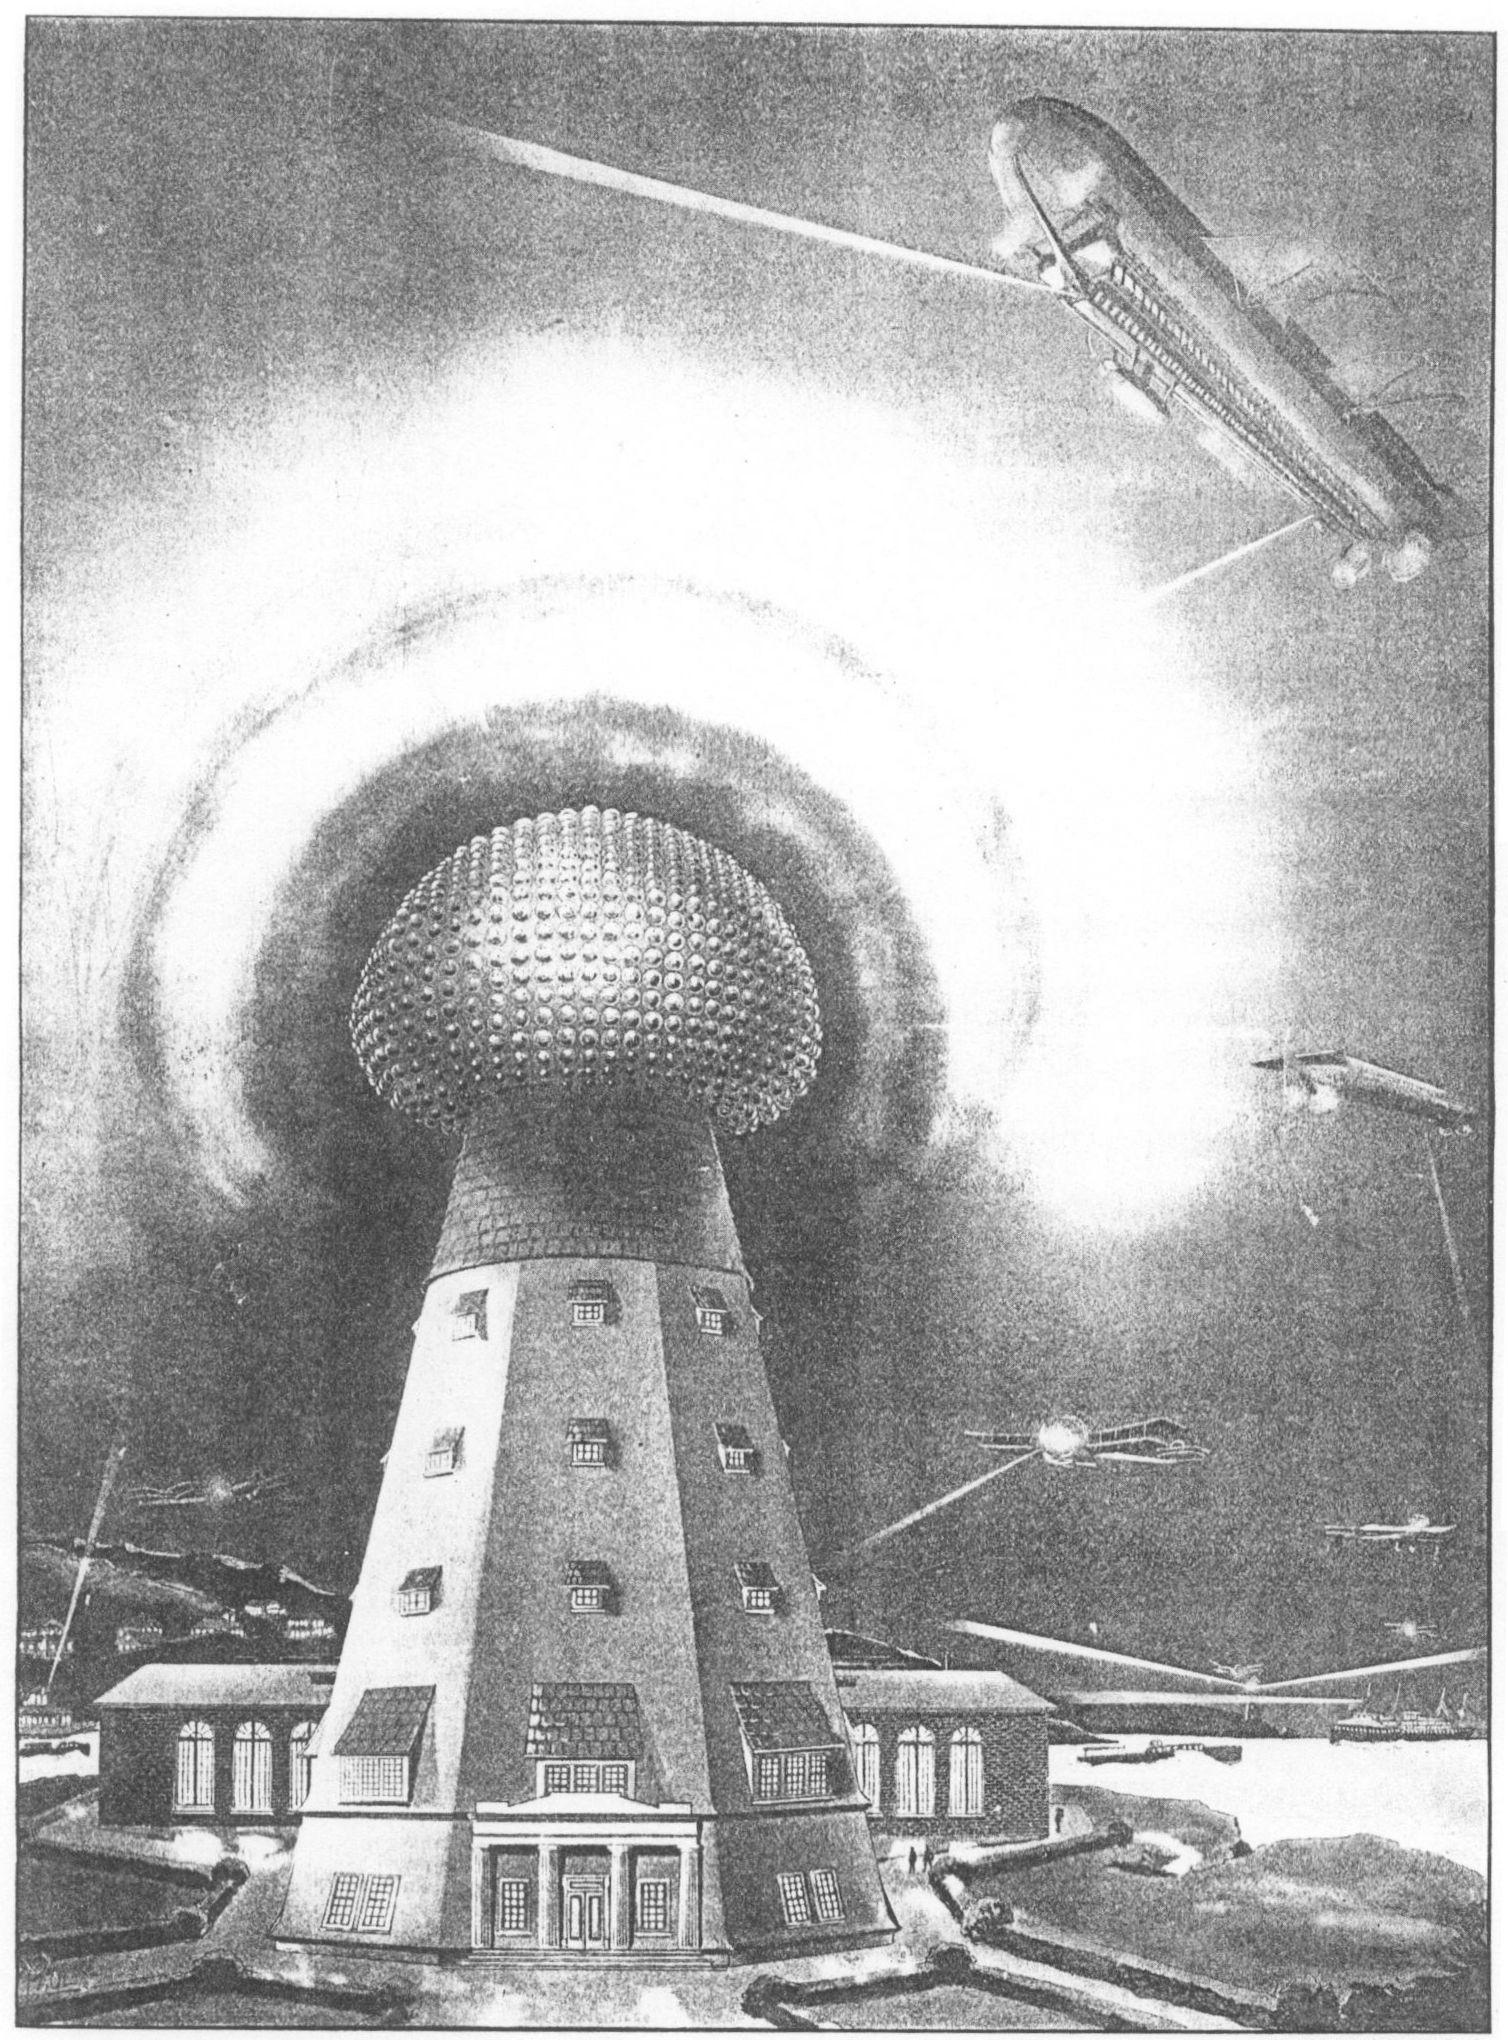
\includegraphics[width=1.3\linewidth]{TowerIsland.png}
	}
	\legend{This photograph of a model shows how the Tesla Tower built on Long Island , eighteen yers ago, would have look completed. From its appearence nobody would infer that it was to be used for the great purposes which are set forth in his accompanying article.}
\end{figure}

\subsection{100 Millions Volts Possible}
Judging from my past experience, as much as 100,000,000 volts are perfectly practicable.  On 
the other hand currents of many thousands of amperes may be obtained in the antenna.  A plant 
of but very moderate dimensions is required for such performances.  Theoretically, a terminal of 
less than 90 feet in diameter is sufficient to develop an electromotive force of that magnitude 
while for antenna currents of from 2,000-4,000 amperes at the usual frequencies it need not be 
larger than 30 feet in diameter.  

In a more restricted meaning this wireless transmitter is one in which the Hertz-wave radiation is 
an entirely negligible quantity as compared with the whole energy, under which condition the 
damping factor is extremely small and an enormous charge is stored in the elevated capacity.  
Such a circuit may then be excited with impulses of any kind, even of low frequency and it will 
yield sinusoidal and continuous oscillations like those of an alternator.  

Taken in the narrowest significance of the term, however, it is a resonant transformer which, 
besides possessing these qualities, is accurately proportioned to fit the globe and its electrical 
constants and properties, by virtue of which design it becomes highly efficient and effective in the 
wireless transmission of energy.  Distance is then absolutely eliminated, there being no 
diminution in the intensity of the transmitted impulses.  It is even possible to make the actions 
increase with the distance from the plant according to an exact mathematical law.  

This invention was one of a number comprised in my "World-System" of wireless transmission 
which I undertook to commercialize on my return to New York in 1900.  As to the immediate 
purposes of my enterprise, they were clearly outlined in a technical statement of that period from 
which I quote: 


{
\itshape 
"The 'World-System' has resulted from a combination of several original 
discoveries made by the 
inventor in the course of long continued research and experimentation.  It makes possible not 
only the instantaneous and precise wireless transmission of any kind of signals, messages or 
characters, to all parts of the world, but also the inter-connection of the existing telegraph, 
telephone, and other signal stations without any change in their present equipment.  By its 
means, for instance, a telephone subscriber here may call up and talk to any other subscriber on 
the Globe.  An inexpensive receiver, not bigger than a watch, will enable him to listen anywhere, 
on land or sea, to a speech delivered or music played in some other place, however distant.  
These examples are cited merely to give an idea of the possibilities of this great scientific 
advance, which annihilates distance and makes that perfect natural conductor, the Earth, 
available for all the innumerable purposes which human ingenuity has found for a line-wire.  One 
far-reaching result of this is that any device capable of being operated thru one or more wires (at 
a distance obviously restricted) can likewise be actuated, without artificial conductors and with the 
same facility and accuracy, at distances to which there are no limits other than those imposed by 
the physical dimensions of the Globe.  Thus, not only will entirely new fields for commercial 
exploitation be opened up by this ideal method of transmission but the old ones vastly extended.  

The 'World-System' is based on the application of the following important inventions and 
discoveries: 
\begin{enumerate}[1.]
\item The 'Tesla Transformer.' This apparatus is in the production of electrical vibrations as 
revolutionary as gunpowder was in warfare.  Currents many times stronger than any ever 
generated in the usual ways, and sparks over one hundred feet long, have been produced by the 
inventor with an instrument of this kind.
\item The 'Magnifying Transmitter.' This is Tesla's best invention, a peculiar transformer specially 
adapted to excite the Earth, which is in the transmission of electrical energy what the telescope is 
in astronomical observation.  By the use of this marvelous device he has already set up electrical 
movements of greater intensity than those of lightning and passed a current, sufficient to light 
more than two hundred incandescent lamps, around the Globe.

\item The 'Tesla Wireless System.' This system comprises a number of improvements and is the 
only means known for transmitting economically electrical energy to a distance without wires.  
Careful tests and measurements in connection with an experimental station of great activity, 
erected by the inventor in Colorado, have demonstrated that power in any desired amount can be 
conveyed, clear across the Globe if necessary, with a loss not exceeding a few per cent.

\item The 'Art of Individualization.' This invention of Tesla's is to primitive 'tuning' what refined 
language is to unarticulated expression.  It makes possible the transmission of signals or 
messages absolutely secret and exclusive both in the active and passive aspect, that is, non-
interfering as well as non-interferable.  Each signal is like an individual of unmistakable identity 
and there is virtually no limit to the number of stations or instruments which can be 
simultaneously operated without the slightest mutual disturbance.

\item 'The Terrestrial Stationary Waves.' This wonderful discovery, popularly explained, means that 
the Earth is responsive to electrical vibrations of definite pitch just as a tuning fork to certain 
waves of sound.  These particular electrical vibrations, capable of powerfully exciting the Globe, 
lend themselves to innumerable uses of great importance commercially and in many other 
respects.
\end{enumerate}

The first 'World-System' power plant can be put in operation in nine months.  With this power 
plant it will be practicable to attain electrical activities up to ten million horsepower and it is 
designed to serve for as many technical achievements as are possible without due expense.  
Among these the following may be mentioned:
\begin{enumerate}[(1)]
\item The inter-connection of the existing telegraph exchanges or offices all over the world;

\item The establishment of a secret and non-interferable government telegraph service;

\item The inter-connection of all the present telephone exchanges or offices on the Globe;

\item The universal distribution of general news, by telegraph or telephone, in connection with the 
Press;

\item The establishment of such a 'World-System' of intelligence transmission for exclusive private 
use;

\item The inter-connection and operation of all stock tickers of the world;

\item The establishment of a 'World-System' of musical distribution, etc.;

\item The universal registration of time by cheap clocks indicating the hour with astronomical 
precision and requiring no attention whatever;

\item The world transmission of typed or handwritten characters, letters, checks, etc.;

\item The establishment of a universal marine service enabling the navigators of all ships to steer 
perfectly without compass, to determine the exact location, hour and speed, to prevent collisions 
and disasters, etc.;

\item The inauguration of a system of world-printing on land and sea;

\item The world reproduction of photographic pictures and all kinds of drawings or records.
\end{enumerate}
}

I also proposed to make demonstrations in the wireless transmission of power on a small scale 
but sufficient to carry conviction.  Besides these I referred to other and incomparably more 
important applications of my discoveries which will be disclosed at some future date.  

A plant was built on Long Island with a tower 187 feet high, having a spherical terminal about 68 
feet in diameter.  These dimensions were adequate for the transmission of virtually any amount of 
energy.  Originally only from 200 to 300 K.W. were provided but I intended to employ later several 
thousand horsepower.  The transmitter was to emit a wave complex of special characteristics and 
I had devised a unique method of telephonic control of any amount of energy.  

The tower was destroyed two years ago but my projects are being developed and another one, 
improved in some features, will be constructed.  On this occasion I would contradict the widely 
circulated report that the structure was demolished by the Government which owing to war 
conditions, might have created prejudice in the minds of those who may not know that the papers, 
which thirty years ago conferred upon me the honor of American citizenship, are always kept in a 
safe, while my orders, diplomas, degrees, gold medals and other distinctions are packed away in 
old trunks.  If this report had a foundation I would have been refunded a large sum of money 
which I expended in the construction of the tower.  On the contrary it was in the interest of the 
Government to preserve it, particularly as it would have made possible—to mention just one 
valuable result—the location of a submarine in any part of the world.  My plant, services, and all 
my improvements have always been at the disposal of the officials and ever since the outbreak of 
the European conflict I have been working at a sacrifice on several inventions of mine relating to 
aerial navigation, ship propulsion and wireless transmission which are of the greatest importance 
to the country.  Those who are well informed know that my ideas have revolutionized the 
industries of the United States and I am not aware that there lives an inventor who has been, in 
this respect, as fortunate as myself especially as regards the use of his improvements in the war.  
I have refrained from publicly expressing myself on this subject before as it seemed improper to 
dwell on personal matters while all the world was in dire trouble.  

I would add further, in view of various rumors which have reached me, that Mr.  J. Pierpont 
Morgan did not interest himself with me in a business way but in the same large spirit in which he 
has assisted many other pioneers.  He carried out his generous promise to the letter and it would 
have been most unreasonable to expect from him anything more.  He had the highest regard for 
my attainments and gave me every evidence of his complete faith in my ability to ultimately 
achieve what I had set out to do.  I am unwilling to accord to some smallminded and jealous 
individuals the satisfaction of having thwarted my efforts.  These men are to me nothing more 
than microbes of a nasty disease.  My project was retarded by laws of nature.  The world was not 
prepared for it.  It was too far ahead of time.  But the same laws will prevail in the end and make it 
a triumphal success.  

\newpage

	\vspace*{\stretch{1}}
	{\centering
		\aldine\\
		\aldine\hspace{1.2em}\aldine
		\par}
	\vspace*{2cm}
	


%%------------------Chapitre 6 ------------------
\cleardoublepage
\thispagestyle{empty}
\markboth{The Art of Telautomatics}{}
\vspace*{5em}
\begin{center}
	\bfseries
	\noindent {\Large\decofourleft~\textsc{VI}~\decofourright}\\
	\noindent\rule{.5\linewidth}{1pt}\\
	\medskip
	{\noindent\LARGE The Art of\\Telautomatics}
	
	\bigskip
	
	
	{\normalfont\smallskip\footnotesize\protect\parbox{.75\linewidth}{\itshape
			\lettrine[lines=2]{I}{n} this article, Dr. Tesla dwells on the future possibilities of his magnifying transmitter, especially in connection with the art of Telautomatics, which was first conceived by him and doubtless constitutes one of his most brillant gifts to the world.
			
			Tesla was the first to build and successfully operate Automata in the form of boats steered and otherwise controlled by tuned wireless circuits and agents ensuring reliable action despite of all attempts to interfere.
			
			But this was only the first step in the evolution of his invention. What he wanted, was to produce machine capable of acting as though possessed of intelligence. It will be readily perceived that if dr. Tesla has practically realized his conception, the world will witness a revolution in every field of endavor. In particular will his inventions affect the art of warfare and the peace of the world.
			
			Dr. Tesla dwells eloquently on a number of topics agitating the public mind, and this article of his is perhaps the most brilliant and absorbing he heas written.\\
			
			\hfill --\scshape{Editor}.
		}
		\par
	}
	\vspace*{5em}
\end{center}

\addtocontents{toc}{\normalsize}
\addcontentsline{toc}{section}{The Art of Telautomatics}

\subsection{How Tesla's Mind Recuperates}

No subject to which I have ever devoted myself has called for such concentration of mind and 
strained to so dangerous a degree the finest fibers of my brain as the system of which the 
Magnifying Transmitter is the foundation.  I put all the intensity and vigor of youth in the 
development of the rotating field discoveries, but those early labors were of a different character.  
Although strenuous in the extreme, they did not involve that keen and exhausting discernment 
which had to be exercised in attacking the many puzzling problems of the wireless.  Despite my 
rare physical endurance at that period the abused nerves finally rebelled and I suffered a 
complete collapse, just as the consummation of the long and difficult task was almost in sight.  

Without doubt I would have paid a greater penalty later, and very likely my career would have 
been prematurely terminated, had not providence equipt me with a safety device, which has 
seemed to improve with advancing years and unfailingly comes into play when my forces are at 
an end.  So long as it operates I am safe from danger, due to overwork, which threatens other 
inventors and, incidentally, I need no vacations which are indispensable to most people.  When I 
am all but used up I simply do as the darkies, who "naturally fall asleep while white folks worry." 
To venture a theory out of my sphere, the body probably accumulates little by little a definite 
quantity of some toxic agent and I sink into a nearly lethargic state which lasts half an hour to the 
minute.  Upon awakening I have the sensation as though the events immediately preceding had 
occurred very long ago, and if I attempt to continue the interrupted train of thought I feel a 
veritable mental nausea.  Involuntarily I then turn to other work and am surprised at the freshness 
of the mind and ease with which I overcome obstacles that had baffled me before.  After weeks or 
months my passion for the temporarily abandoned invention returns and I invariably find answers 
to all the vexing questions with scarcely any effort.  

In this connection I will tell of an extraordinary experience which may be of interest to students of 
psychology.  I had produced a striking phenomenon with my grounded transmitter and was 
endeavoring to ascertain its true significance in relation to the currents propagated through the 
earth.  It seemed a hopeless undertaking, and for more than a year I worked unremittingly, but in 
vain.  This profound study so entirely absorbed me that I became forgetful of everything else, 
even of my undermined health.  At last, as I was at the point of breaking down, nature applied the 
preservative inducing lethal sleep.  Regaining my senses I realized with consternation that I was 
unable to visualize scenes from my life except those of infancy, the very first ones that had 
entered my consciousness.  Curiously enough, these appeared before my vision with startling 
distinctness and afforded me welcome relief.  Night after night, when retiring, I would think of 
them and more and more of my previous existence was revealed.  The image of my mother was 
always the principal figure in the spectacle that slowly unfolded, and a consuming desire to see 
her again gradually took possession of me.  This feeling grew so strong that I resolved to drop all 
work and satisfy my longing.  But I found it too hard to break away from the laboratory, and 
several months elapsed during which I had succeeded in reviving all the impressions of my past 
life up to the spring of 1892.  In the next picture that came out of the mist of oblivion, I saw myself 
at the Hotel de la Paix in Paris just coming to from one of my peculiar sleeping spells, which had 
been caused by prolonged exertion of the brain.  Imagine the pain and distress I felt when it 
flashed upon my mind that a dispatch was handed to me at that very moment bearing the sad 
news that my mother was dying.  I remembered how I made the long journey home without an 
hour of rest and how she passed away after weeks of agony! It was especially remarkable that 
during all this period of partially obliterated memory I was fully alive to everything touching on the 
subject of my research.  I could recall the smallest details and the least significant observations in 
my experiments and even recite pages of text and complex mathematical formulae.  

\begin{figure}[b]
	\centering
	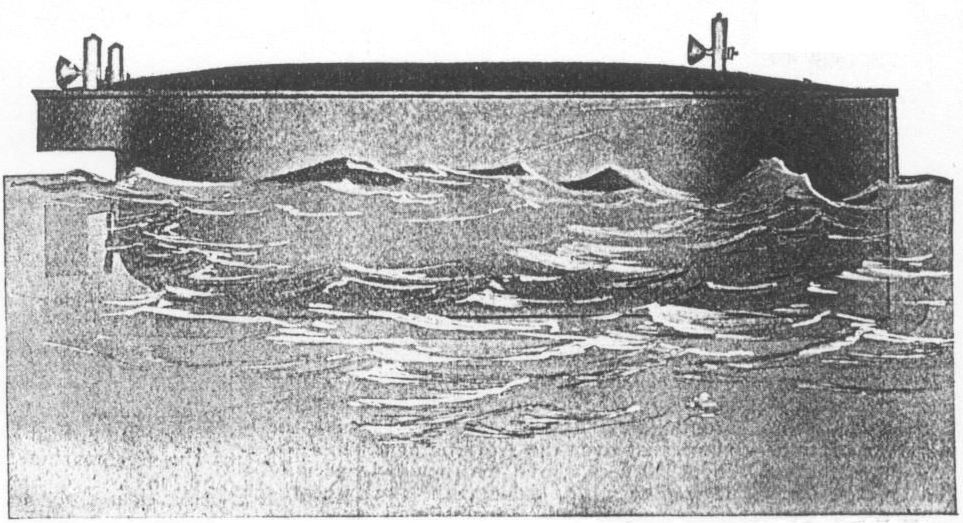
\includegraphics[width=.75\textwidth]{TelBoat.png}
	\legend{One of the Telautomatic Boats (submersible) Constructed by Tesla and Exhibited by Him in 1898. Controlled by Wireless without Aerials.}
\end{figure}

My belief is firm in a law of compensation.  The true rewards are ever in proportion to the labor 
and sacrifices made.  This is one of the reasons why I feel certain that of all my inventions, the 
Magnifying Transmitter will prove most important and valuable to future generations.  I am 
prompted to this prediction not so much by thoughts of the commercial and industrial revolution 
which it will surely bring about, but of the humanitarian consequences of the many achievements 
it makes possible.  Considerations of mere utility weigh little in the balance against the higher 
benefits of civilization.  We are confronted with portentous problems which can not be solved just 
by providing for our material existence, however abundantly.  On the contrary, progress in this 
direction is fraught with hazards and perils not less menacing than those born from want and 
suffering.  If we were to release the energy of atoms or discover some other way of developing 
cheap and unlimited power at any point of the globe this accomplishment, instead of being a 
blessing, might bring disaster to mankind in giving rise to dissension and anarchy which would 
ultimately result in the enthronement of the hated regime of force.  The greatest good will comes 
from technical improvements tending to unification and harmony, and my wireless transmitter is 
preeminently such.  By its means the human voice and likeness will be reproduced everywhere 
and factories driven thousands of miles from waterfalls furnishing the power; aerial machines will 
be propelled around the earth without a stop and the sun's energy controlled to create lakes and 
rivers for motive purposes and transformation of arid deserts into fertile land.  Its introduction for 
telegraphic, telephonic and similar uses will automatically cut out the statics and all other 
interferences which at present impose narrow limits to the application of the wireless. This is a timely topic on which a few words might not be amiss.   



\subsection{Tesla Rapes "Static`` Men Vigorously}
During the past decade a number 
of people have arrogantly claimed that they had succeeded in doing away with this impediment.  I 
have carefully examined all of the arrangements described and tested most of them long before 
they were publicly disclosed, but the finding was uniformly negative.  A recent official statement 
from the U.S. Navy may, perhaps, have taught some beguilable news editors how to appraise 
these announcments at their real worth.  As a rule the attempts are based on theories so 
fallacious that whenever they come to my notice I can not help thinking in a lighter vein.  Quite 
recently a new discovery was heralded, with a deafening flourish of trumpets, but it proved 
another case of a mountain bringing forth a mouse.  

This reminds me of an exciting incident which took place years ago when I was conducting my 
experiments with currents of high frequency.  Steve Brodie had just jumped off the Brooklyn 
Bridge.  The feat has been vulgarized since by imitators, but the first report electrified New York.  
I was very impressionable then and frequently spoke of the daring printer.  On a hot afternoon I 
felt the necessity of refreshing myself and stepped into one of the popular thirty thousand 
institutions of this great city where a delicious twelve per cent beverage was served which can 
now be had only by making a trip to the poor and devastated countries of Europe.  The 
attendance was large and not overdistinguished and a matter was discussed which gave me an 
admirable opening for the careless remark: "This is what I said when I jumped off the bridge." No 
sooner had I uttered these words than I felt like the companion of Timotheus in the poem of 
Schiller.  In an instant there was a pandemonium and a dozen voices cried: "It is Brodie! " I threw 
a quarter on the counter and bolted for the door but the crowd was at my heels with yells: "Stop, 
Steve!" which must have been misunderstood for many persons tried to hold me up as I ran 
frantically for my haven of refuge.  By darting around corners I fortunately managed - through the 
medium of a fire-escape - to reach the laboratory where I threw off my coat, camouflaged myself 
as a hard-working blacksmith, and started the forge.  But these precautions proved unnecessary; 
I had eluded my pursuers.  For many years afterward, at night, when imagination turns into 
spectres the trifling troubles of the day, I often thought, as I tossed on the bed, what my fate 
would have been had that mob caught me and found out that I was not Steve Brodie! 


Now the engineer, who lately gave an account before a technical body of a novel remedy against 
statics based on a "heretofore unknown law of nature," seems to have been as reckless as 
myself when he contended that these disturbances propagate up and down, while those of a 
transmitter proceed along the earth.  It would mean that a condenser, as this globe, with its 
gaseous envelope, could be charged and discharged in a manner quite contrary to the 
fundamental teachings propounded in every elemental text-book of physics.  Such a supposition 
would have been condemned as erroneous, even in Franklin's time, for the facts bearing on this 
were then well known and the identity between atmospheric electricity and that developed by 
machines was fully established. 

 Obviously, natural and artificial disturbances propagate through 
the earth and the air in exactly the same way, and both set up electromotive forces in the 
horizontal, as well as vertical, sense.  Interference can not be overcome by any such methods as 
were proposed.  The truth is this: in the air the potential increases at the rate of about fifty volts 
per foot of elevation, owing to which there may be a difference of pressure amounting to twenty, 
or even forty thousand volts between the upper and lower ends of the antenna.  The masses of 
the charged atmosphere are constantly in motion and give up electricity to the conductor, not 
continuously but rather disruptively, this producing a grinding noise in a sensitive telephonic 
receiver.  The higher the terminal and the greater the space encompassed by the wires, the more 
pronounced is the effect, but it must be understood that it is purely local and has little to do with 
the real trouble.  

In 1900, while perfecting my wireless system, one form of apparatus comprised four antennae.  
These were carefully calibrated to the same frequency and connected in multiple with the object 
of magnifying the action, in receiving from any direction.  When I desired to ascertain the origin of 
the transmitted impulses, each diagonally situated pair was put in series with a primary coil 
energizing the detector circuit.  In the former case the sound was loud in the telephone; in the 
latter it ceased, as expected, the two antennae neutralizing each other, but the true statics 
manifested themselves in both instances and I had to devise special preventives embodying 
different principles.  

\subsection{The Remedy for Static}
\emph{By employing receivers connected to two points of the ground, as suggested by me long ago, this 
trouble caused by the charged air, which is very serious in the structures as now built, is nullified} 
and besides, the liability of all kinds of interference is reduced to about one-half, because of the 
directional character of the circuit.  This was perfectly self-evident, but came as a revelation to 
some simple-minded wireless folks whose experience was confined to forms of apparatus that 
could have been improved with an axe, and they have been disposing of the bear's skin before 
killing him.  If it were true that strays performed such antics, it would be easy to get rid of them by 
receiving without aerials.  But, as a matter of fact, a wire buried in the ground which, conforming 
to this view, should be absolutely immune, is more susceptible to certain extraneous impulses 
than one placed vertically in the air.  To state it fairly, a slight progress has been made, but not by 
virtue of any particular method or device.  It was achieved simply by discarding the enormous 
structures, which are bad enough for transmission but wholly unsuitable for reception, and 
adopting a more appropriate type of receiver.  As I pointed out in a previous article, to dispose of 
this difficulty for good, a radical change must be made in the system, and the sooner this is done 
the better.  


\begin{figure}[p]
	\vspace*{-2cm}
	\makebox[\linewidth]{
		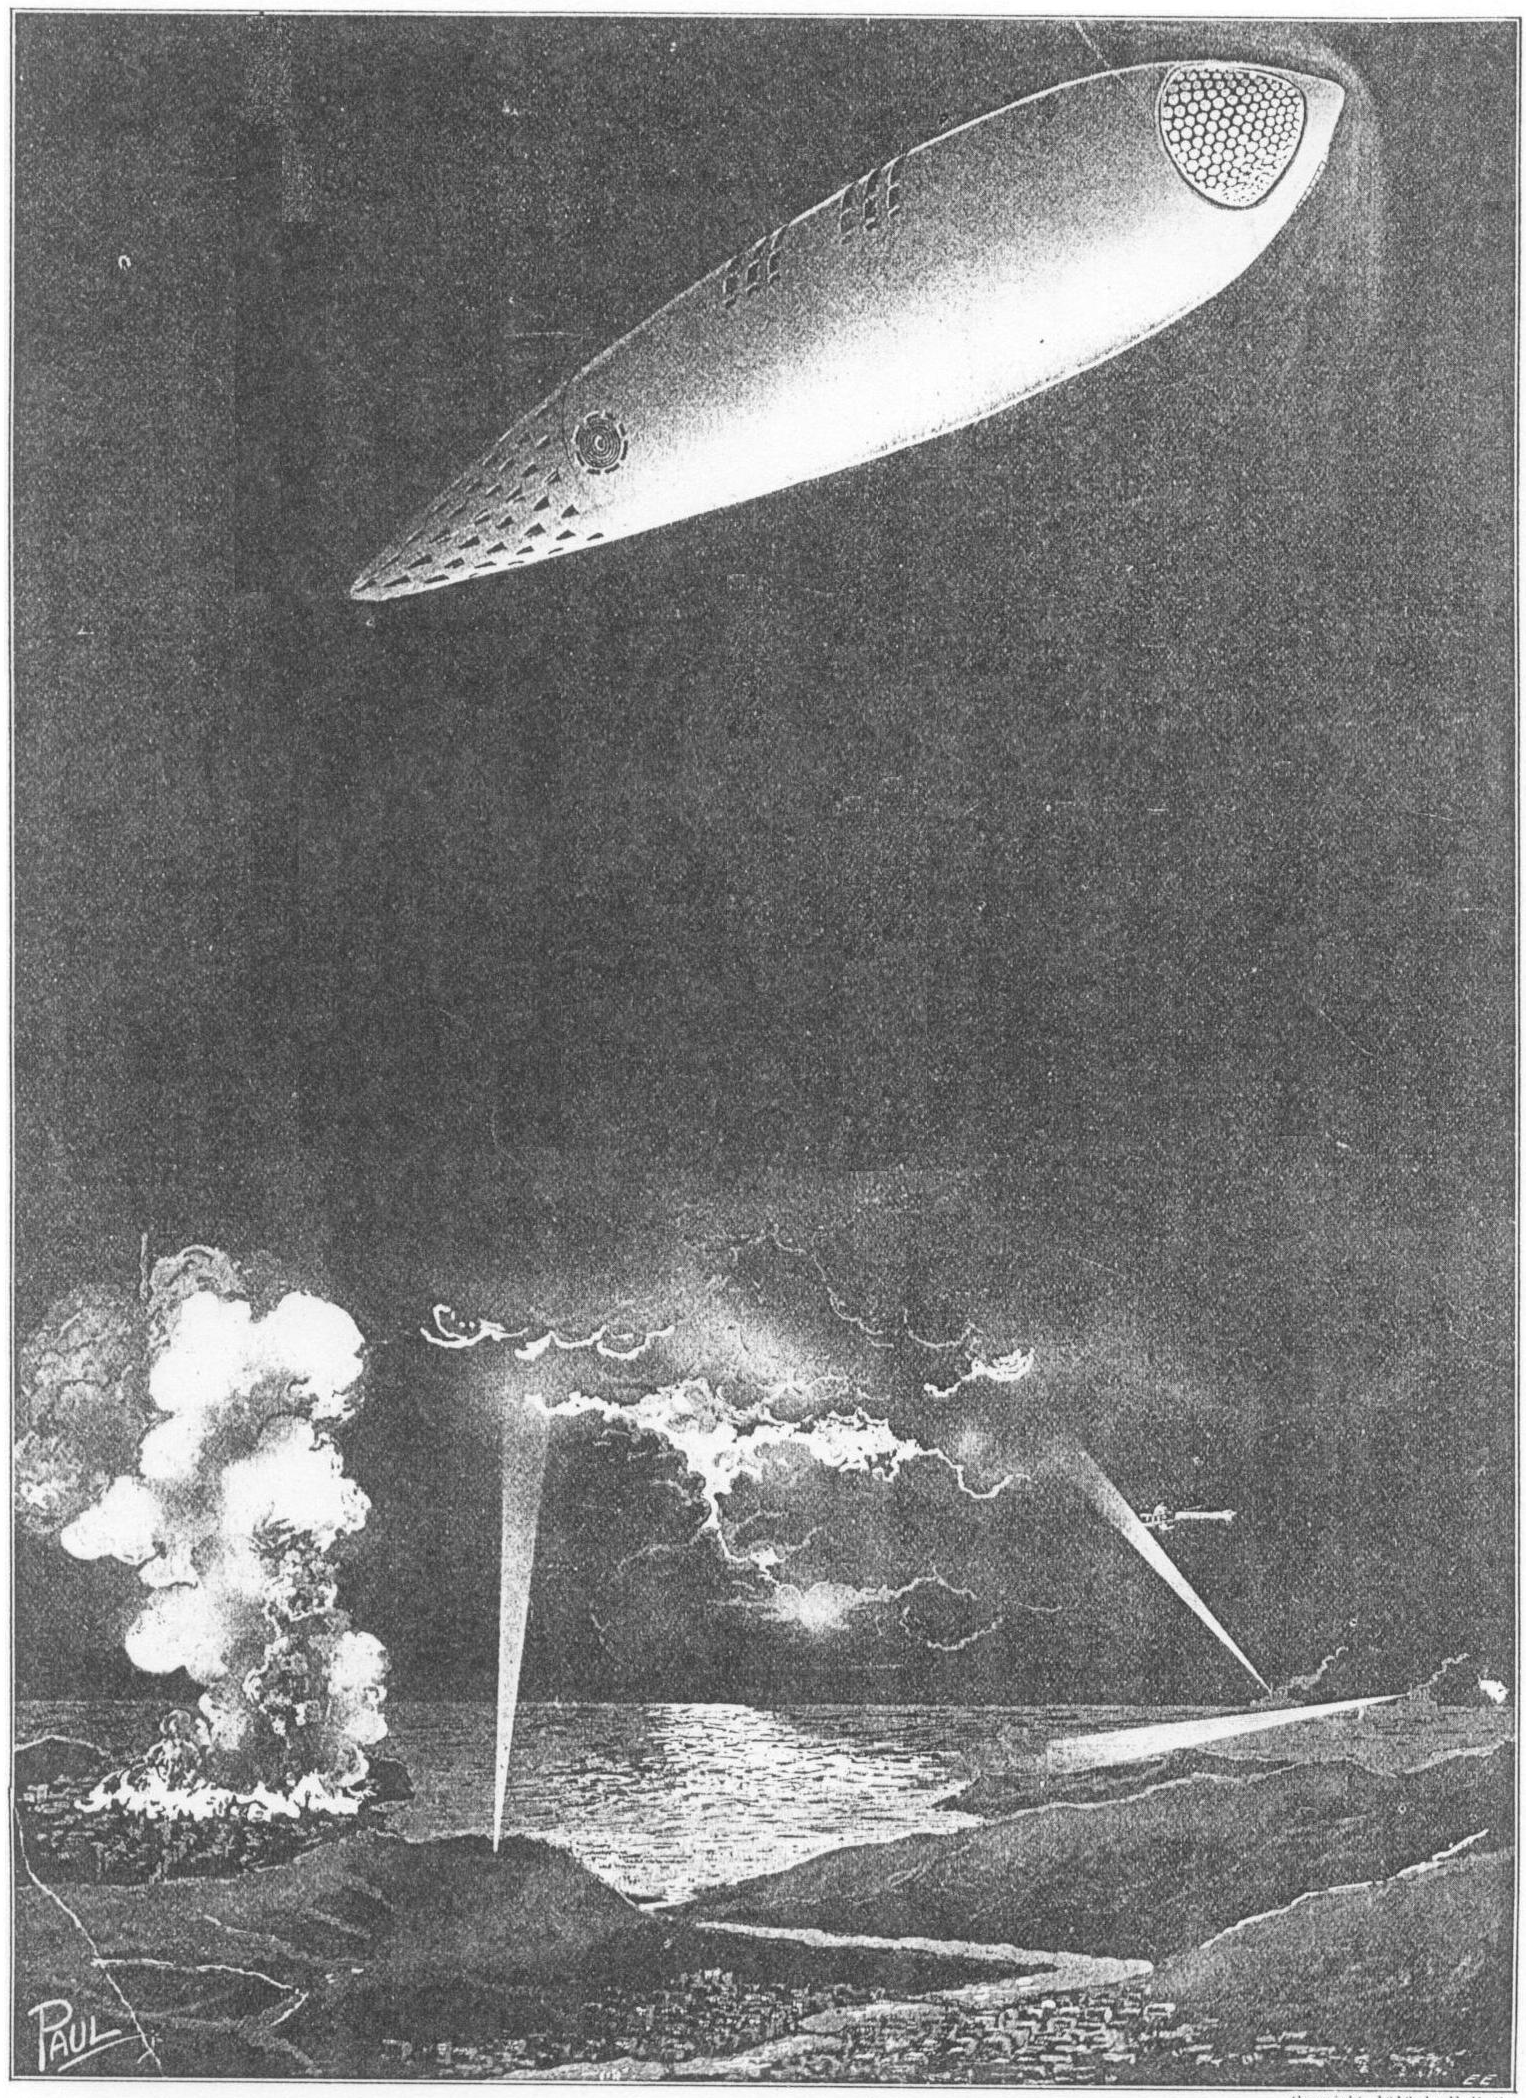
\includegraphics[width=1.3\linewidth]{TelAer.png}
	}
	\legend{Tesla's new S. If-Propelled Aerial Tel-Automaton. Devold of propeller, substaining wings and all other means of external control. Can attain a speed of $350$ Miles per Hour, and will reac a predetermined point a thousand Miles away accurately within a few feet.}
\end{figure}

\subsection{Radio Government Control Not Wanted}
It would be calamitous, indeed, if at this time when the art is in its infancy and the vast majority, 
not excepting even experts, have no conception of its ultimate possibilities, a measure would be 
rushed through the legislature making it a government monopoly.  This was proposed a few 
weeks ago by Secretary Daniels, and no doubt that distinguished official has made his appeal to 
the Senate and House of Representatives with sincere conviction.  But universal evidence 
unmistakably shows that the best results are always obtained in healthful commercial 
competition.  There are, however, exceptional reasons why wireless should be given the fullest 
freedom of development.  In the first place it offers prospects immeasurably greater and more 
vital to betterment of human life than any other invention or discovery in the history of man.  Then 
again, it must be understood that this wonderful art has been, in its entirety, evolved here and can 
be called "American" with more right and propriety than the telephone, the incandescent lamp or 
the aeroplane.  Enterprising press agents and stock jobbers have been so successful in 
spreading misinformation that even so excellent a periodical as the Scientific American accords 
the chief credit to a foreign country.  The Germans, of course, gave us the Hertz-waves and the 
Russian, English, French and Italian experts were quick in using them for signaling purposes.  It 
was an obvious application of the new agent and accomplished with the old classical and 
unimproved induction coil - scarcely anything more than another kind of heliography.  The radius 
of transmission was very limited, the results attained of little value, and the Hertz oscillations, as a 
means for conveying intelligence, could have been advantageously replaced by sound-waves, 
which I advocated in 1891.  Moreover, all of these attempts were made three years after the basic 
principles of the wireless system, which is universally employed to-day, and its potent 
instrumentalities had been clearly described and developed in America.  No trace of those 
Hertzian appliances and methods remains today.  We have proceeded in the very opposite 
direction and what has been done is the product of the brains and efforts of citizens of this 
country.  The fundamental patents have expired and the opportunities are open to all.  The chief 
argument of the Secretary is based on interference.  According to his statement, reported in the 
New York Herald of July 29th, signals from a powerful station can be intercepted in every village 
of the world .  In view of this fact, which was demonstrated in my experiments of 1900, it would be 
of little use to impose restrictions in the United States.  


\subsection{America First}
As throwing light on this point, I may mention that only recently an odd looking gentleman called 
on me with the object of enlisting my services in the construction of world transmitters in some 
distant land.  "We have no money," he said, "but carloads of solid gold and we will give you a 
liberal amount." I told him that I wanted to see first what will be done with my inventions in 
America, and this ended the interview.  But I am satisfied that some dark forces are at work, and 
as time goes on the maintenance of continuous communication will be rendered more difficult.  
The only remedy is a system immune against interruption.  It has been perfected, it exists, and all 
that is necessary is to put it in operation.  

The terrible conflict is still uppermost in the minds and perhaps the greatest importance will be 
attached to the Magnifying Transmitter as a machine for attack and defense, more particularly in 
connection with Telautomatics.  This invention is a logical outcome of observations begun in my 
boyhood and continued thruout my life.  When the first results were publisht the Electrical Review 
stated editorially that it would become one of the "most potent factors in the advance and 
civilization of mankind." The time is not distant when this prediction will be fulfilled.  In 1898 and 
1900 it was offered to the Government and might have been adopted were I one of those who 
would go to Alexander's shepherd when they want a favor from Alexander.  At that time I really 
thought that it would abolish war, because of its unlimited destructiveness and exclusion of the 
personal element of combat.  But while I have not lost faith in its potentialities, my views have 
changed since.  


\subsection{The Road To Permanent Peace}
War can not be avoided until the physical cause for its recurrence is removed and this, in the last 
analysis, is the vast extent of the planet on which we live.  Only thru annihilation of distance in 
every respect, as the conveyance of intelligence, transport of passengers and supplies and 
transmission of energy will conditions be brought about some day, insuring permanency of 
friendly relations.  What we now want most is closer contact and better understanding between 
individuals and communities all over the earth, and the elimination of that fanatic devotion to 
exalted ideals of national egoism and pride which is always prone to plunge the world into 
primeval barbarism and strife.  No league or parliamentary act of any kind will ever prevent such 
a calamity.  These are only new devices for putting the weak at the mercy of the strong.  I have 
exprest myself in this regard fourteen years ago, when a combination of a few leading 
governments - a sort of Holy Alliance - was advocated by the late Andrew Carnegie, who may be 
fairly considered as the father of this idea, having given to it more publicity and impetus than 
anybody else prior to the efforts of the President.  While it can not be denied that such a pact 
might be of material advantage to some less fortunate peoples, it can not attain the chief object 
sought.  Peace can only come as a natural consequence of universal enlightenment and merging 
of races, and we are still far from this blissful realization.  

As I view the world of today, in the light of the gigantic struggle we have witnest, I am filled with 
conviction that the interests of humanity would be best served if the United States remained true 
to its traditions and kept out of "entangling alliances." Situated as it is, geographically, remote 
from the theaters of impending conflicts, without incentive to territorial aggrandizement, with 
inexhaustible resources and immense population thoroly imbued with the spirit of liberty and right, 
this country is placed in a unique and privileged position.  It is thus able to exert, independently, 
its colossal strength and moral force to the benefit of all, more judiciously and effectively, than as 
member of a league.  


\subsection{The Mechanistic Theory Of Life}
In one of these biographical sketches, published in the \textsc{Electrical Experimenter}, I have 
dwelt on the circumstances of my early life and told of an affliction which compelled me to 
unremitting exercise of imagination and self observation.  This mental activity, at first involuntary 
under the pressure of illness and suffering, gradually became second nature and led me finally to 
recognize that I was but an automaton devoid of free will in thought and action and merely 
responsive to the forces of the environment.  Our bodies are of such complexity of structure, the 
motions we perform are so numerous and involved, and the external impressions on our sense 
organs to such a degree delicate and elusive that it is hard for the average person to grasp this 
fact.  And yet nothing is more convincing to the trained investigator than the mechanistic theory of 
life which had been, in a measure, understood and propounded by Descartes three hundred 
years ago.  But in his time many important functions of our organism were unknown and, 
especially with respect to the nature of light and the construction and operation of the eye, 
philosophers were in the dark.  

In recent years the progress of scientific research in these fields has been such as to leave no 
room for a doubt in regard to this view on which many works have been published.  One of its 
ablest and most eloquent exponents is, perhaps, Felix Le Dantec, formerly assistant of Pasteur.  
Prof. Jacques Loeb has performed remarkable experiments in heliotropism, clearly establishing 
the controlling power of light in lower forms of organisms, and his latest book, "Forced 
Movements," is revelatory.  But while men of science accept this theory simply as any other that 
is recognized, to me it is a truth which I hourly demonstrate by every act and thought of mine.  
The consciousness of the external impression prompting me to any kind of exertion, physical or 
mental, is ever present in my mind.  Only on very rare occasions, when I was in a state of 
exceptional concentration, have I found difficulty in locating the original impulses.  

\subsection{Lack of Observation a Form of Ignorance}
The by far greater number of human beings are never aware of what is passing around and within 
them, and millions fall victims of disease and die prematurely just on this account.  The 
commonest every-day occurrences appear to them mysterious and inexplicable.  One may feel a 
sudden wave of sadness and rake his brain for an explanation when he might have noticed that it 
was caused by a cloud cutting off the rays of the sun.  He may see the image of a friend dear to 
him under conditions which he construes as very peculiar, when only shortly before he has 
passed him in the street or seen his photograph somewhere.  When he loses a collar button he 
fusses and swears for an hour, being unable to visualize his previous actions and locate the 
object directly.  Deficient observation is merely a form of ignorance and responsible for the many 
morbid notions and foolish ideas prevailing.  There is not more than one out of every ten persons 
who does not believe in telepathy and other psychic manifestations, spiritualism and communion 
with the dead, and who would refuse to listen to willing or unwilling deceivers.  

Just to illustrate how deeply rooted this tendency has become even among the clearheaded 
American population, I may mention a comical incident.  

\subsection{Psychic Phenomena in the Manufacture of Flivvers}
Shortly before the war, when the 
exhibition of my turbines in this city elicited widespread comment in the technical papers, I 
anticipated that there would.  be a scramble among manufacturers to get hold of the invention, 
and I had particular designs on that man from Detroit who has an uncanny faculty for 
accumulating millions.  So confident was I that he would turn up some day, that I declared this as 
certain to my secretary and assistants.  Sure enough, one fine morning a body of engineers from 
the Ford Motor Company presented themselves with the request of discussing with me an 
important project.  "Didn't I tell you?" I remarked triumphantly to my employees, and one of them 
said, "You are amazing, Mr. Tesla; everything comes out exactly as you predict." As soon as 
these hard-headed men were seated I, of course, immediately began to extol the wonderful 
features of my turbine, when the spokesmen interrupted me and said, "We know all about this, 
but we are on a special errand.  We have formed a psychological society for the investigation of 
psychic phenomena and we want you to join us in this undertaking." I suppose those engineers 
never knew how near they came to being fired out of my office.  

\subsection{Confuting Spiritism}
Ever since I was told by some of the greatest men of the time, leaders in science whose names 
are immortal, that I am possesst of an unusual mind, I bent all my thinking faculties on the 
solution of great problems regardless of sacrifice.  For many years I endeavored to solve the 
enigma of death, and watched eagerly for every kind of spiritual indication.  But only once in the 
course of my existence have I had an experience which momentarily impressed me as 
supernatural.  It was at the time of my mother's death.  I had become completely exhausted by 
pain and long vigilance, and one night was carried to a building about two blocks from our home.  
As I lay helpless there, I thought that if my mother died while I was away from her bedside she 
would surely give me a sign.  Two or three months before I was in London in company with my 
late friend, Sir William Crookes, when spiritualism was discussed, and I was under the full sway 
of these thoughts.  I might not have paid attention to other men, but was susceptible to his 
arguments as it was his epochal work on radiant matter, which I had read as a student, that made 
me embrace the electrical career.  I reflected that the conditions for a look into the beyond were 
most favorable, for my mother was a woman of genius and particularly excelling in the powers of 
intuition.  During the whole night every fiber in my brain was strained in expectancy, but nothing 
happened until early in the morning, when I fell in a sleep, or perhaps a swoon, and saw a cloud 
carrying angelic figures of marvelous beauty, one of whom gazed upon me lovingly and gradually 
assumed the features of my mother.  The appearance slowly floated across the room and 
vanished, and I was awakened by an indescribably sweet song of many voices.  In that instant a 
certitude, which no words can express, came upon me that my mother had just died.  And that 
was true.  I was unable to understand the tremendous weight of the painful knowledge I received 
in advance, and wrote a letter to Sir William Crookes while still under the domination of these 
impressions and in poor bodily health.  When I recovered I sought for a long time the external 
cause of this strange manifestation and, to my great relief, I succeeded after many months of 
fruitless effort.  I had seen the painting of a celebrated artist, representing allegorically one of the 
seasons in the form of a cloud with a group of angels which seemed to actually float in the air, 
and this had struck me forcefully.  It was exactly the same that appeared in my dream, with the 
exception of my mother's likeness.  The music came from the choir in the church nearby at the 
early mass of Easter morning, explaining everything satisfactorily in conformity with scientific 
facts.  

This occurred long ago, and I have never had the faintest reason since to change my views on 
psychical and spiritual phenomena, for which there is absolutely no foundation.  The belief in 
these is the natural outgrowth of intellectual development.  Religious dogmas are no longer 
accepted in their orthodox meaning, but every individual clings to faith in a supreme power of 
some kind.  We all must have an ideal to govern our conduct and insure contentment, but it is 
immaterial whether it be one of creed, art, science or anything else, so long as it fulfills the 
function of a dematerializing force.  It is essential to the peacef ul existence of humanity as a 
whole that one common conception should prevail.  

\subsection{Tesla's Astounding Discovery}
While I have failed to obtain any evidence in support of the contentions of psychologists and 
spiritualists, I have proved to my complete satisfaction the automatism of life, not only through 
continuous observations of individual actions, but even more conclusively through certain 
generalizations.  These amount to a discovery which I consider of the greatest moment to human 
society, and on which I shall briefly dwell.  I got the first inkling of this astounding truth when I was 
still a very young man, but for many years I interpreted what I noted simply as coincidences.  
Namely, whenever either myself or a person to whom I was attached, or a cause to which I was 
devoted, was hurt by others in a particular way, which might be best popularly characterized as 
the most unfair imaginable, I experienced a singular and undefinable pain which, for want of a 
\begin{wrapfigure}{r}{0.65\textwidth}
	\vspace{-20pt}
	\begin{center}
		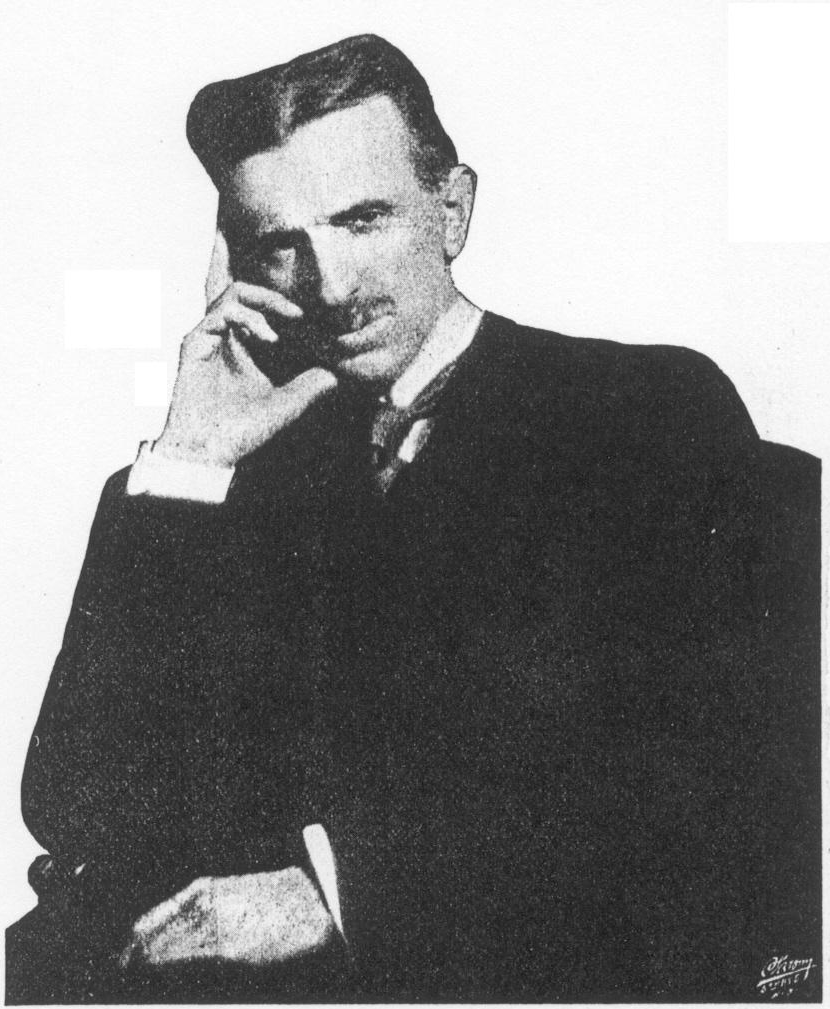
\includegraphics[width=0.63\textwidth]{Tesla-Younger.png}
	\end{center}
	\legend{Dr. Tesla is Rapidly Becoming Younger. Judge for Yourself from his Latest Photograph [circa 1919].}
	\vspace{-20pt}
\end{wrapfigure}
better term, I have qualified as "cosmic," and shortly thereafter, and invariably, those who had 
inflicted it came to grief.  After many such cases I confided this to a number of friends, who had 
the opportunity to convince themselves of the truth of the theory which I have gradually 
formulated and which may be stated in the following few words: 

Our bodies are of similar construction and exposed to the same external influences.  This results 
in likeness of response and concordance of the general activities on which all our social and other 
rules and laws are based.  We are automata entirely controlled by the forces of the medium being 
tossed about like corks on the surface of the water, but mistaking the resultant of the impulses 
from the outside for free will.  The movements and other actions we perform are always life 
preservative and tho seemingly quite independent from one another, we are connected by 
invisible links.  So long as the organism is in perfect order it responds accurately to the agents 
that prompt it, but the moment that there is some derangement in any individual, his self-
preservative power is impaired.  Everybody understands, of course, that if one becomes deaf, 
has his eyesight weakened, or his limbs injured, the chances for his continued existence are 
lessened.  But this is also true, and perhaps more so, of certain defects in the brain which deprive 
the automaton, more or less, of that vital quality and cause it to rush into destruction.  A very 
sensitive and observant being, with his highly developed mechanism all intact, and acting with 
precision in obedience to the changing conditions of the environment, is endowed with a 
transcending mechanical sense, enabling him to evade perils too subtle to be directly perceived.  
When he comes in contact with others whose controlling organs are radically faulty, that sense 
asserts itself and he feels the "cosmic" pain.  The truth of this has been borne out in hundreds of 
instances and I am inviting other students of nature to devote attention to this subject, believing 
that thru combined and systematic effort results of incalculable value to the world will be attained.  

\subsection{Dr. Tesla's First Automaton}
The idea of constructing an automaton, to bear out my theory, presented itself to me early but I 
did not begin active work until 1893, when I started my wireless investigations.  During the 
succeeding two or three years a number of automatic mechanisms, to be actuated from a 
distance, were constructed by me and exhibited to visitors in my laboratory.  In 1896, however, I 
designed a complete machine capable of a multitude of operations, but the consummation of my 
labors was delayed until late in 1897.  This machine was illustrated and described in my article in 
the Century Magazine of June, 1900, and other periodicals of that time and, when first shown in 
the beginning of 1898, it created a sensation such as no other invention of mine has ever 
produced.  In November, 1898, a basic patent on the novel art was granted to me, but only after 
the Examiner-in-Chief had come to New York and witnesst the performance, for what I claimed 
seemed unbelievable.  I remember that when later I called on an official in Washington, with a 
view of offering the invention to the Government, he burst out in laughter upon my telling him 
what I had accomplished.  Nobody thought then that there was the faintest prospect of perfecting 
such a device.  It is unfortunate that in this patent, following the advice of my attorneys, I 
indicated the control as being effected thru the medium of a single circuit and a well-known form 
of detector, for the reason that I had not yet secured protection on my methods and apparatus for 
individualization.  As a matter of fact, my boats were controlled thru the joint action of several 
circuits and interference of every kind was excluded.  Most generally I employed receiving circuits 
in the form of loops, including condensers, because the discharges of my high-tension transmitter 
ionized the air in the hall so that even a very small aerial would draw electricity from the 
surrounding atmosphere for hours.  Just to give an idea, I found, for instance, that a bulb 12" in 
diameter, highly exhausted, and with one single terminal to which a short wire was attached, 
would deliver well on to one thousand successive flashes before all charge of the air in the 
laboratory was neutralized.  The loop form of receiver was not sensitive to such a disturbance 
and it is curious to note that it is becoming popular at this late date.  In reality it collects much less 
energy than the aerials or a long grounded wire, but it so happens that it does away with a 
number of defects inherent to the present wireless devices.  In demonstrating my invention before 
audiences, the visitors were requested to ask any questions, however involved, and the 
automaton would answer them by signs.  This was considered magic at that time but was 
extremely simple, for it was myself who gave the replies by means of the device.  

At the same period another larger telautomatic boat was constructed a photograph of which is 
shown in this number of the \textsc{Electrical Experimenter}.  It was controlled by loops, having 
several turns placed in the hull, which was made entirely water-tight and capable of 
submergence.  The apparatus was similar to that used in the first with the exception of certain 
special features I introduced as, for example, incandescent lamps which afforded a visible 
evidence of the proper functioning of the machine.  

\subsection{Telautomatics of the Future}
These automata, controlled within the range of vision of the operator, were, however, the first and 
rather crude steps in the evolution of the Art of Telautomatics as I had conceived it.  The next 
logical improvement was its application to automatic mechanisms beyond the limits of vision and 
at great distance from the center of control, and I have ever since advocated their employment as 
instruments of warfare in preference to guns.  The importance of this now seems to be 
recognized, if I am to judge from casual announcements thru the press of achievements which 
are said to be extraordinary but contain no merit of novelty, whatever.  In an imperfect manner it 
is practicable, with the existing wireless plants, to launch an aeroplane, have it follow a certain 
approximate course, and perform some operation at a distance of many hundreds of miles.  A 
machine of this kind can also be mechanically controlled in several ways and I have no doubt that 
it may prove of some usefulness in war.  But there are, to my best knowledge, no 
instrumentalities in existence today with which such an object could be accomplished in a precise 
manner.  I have devoted years of study to this matter and have evolved means, making such and 
greater wonders easily realizable.  

As stated on a previous occasion, when I was a student at college I conceived a flying machine 
quite unlike the present ones.  The underlying principle was sound but could not be carried into 
practice for want of a prime-mover of sufficiently great activity.  In recent years I have 
successfully solved this problem and am now planning aerial machines devoid of sustaining 
planes, ailerons, propellers and other external attachments, which will be capable of immense 
speeds and are very likely to furnish powerful arguments for peace in the near future.  Such a 
machine, sustained and propelled entirely by reaction, is shown on page 108 and is supposed to 
be controlled either mechanically or by wireless energy.  By installing proper plants it will be 
practicable to project a missile of this kind into the air and drop it almost on the very spot 
designated, which may be thousands of miles away.  But we are not going to stop at this.  
Telautomata will be ultimately produced, capable of acting as if possest of their own intelligence, 
and their advent will create a revolution.  As early as 1898 I proposed to representatives of a 
large manufacturing concern the construction and public exhibition of an automobile carriage 
which, left to itself, would perform a great variety of operations involving something akin to 
judgment.  But my proposal was deemed chimerical at that time and nothing came from it.  

At present many of the ablest minds are trying to devise expedients for preventing a repetition of 
the awful conflict which is only theoretically ended and the duration and main issues of which I 
have correctly predicted in an article printed in the Sun of December 20, 1914.  The proposed 
League is not a remedy but on the contrary, in the opinion of a number of competent men, may 
bring about results just the opposite.  It is particularly regrettable that a punitive policy was 
adopted in framing the terms of peace, because a few years hence it will be possible for nations 
to fight without armies, ships or guns, by weapons far more terrible, to the destructive action and 
range of which there is virtually no limit.  A city, at any distance whatsoever from the enemy, can 
be destroyed by him and no power on earth can stop him from doing so.  If we want to avert an 
impending calamity and a state of things which may transform this globe into an inferno, we 
should push the development of flying machines and wireless transmission of energy without an 
instant's delay and with all the power and resources of the nation.

	\vspace*{\stretch{1}}
	{\centering
		\aldine\\
		\aldine\hspace{1.2em}\aldine
		\par}
	\vspace*{2cm}
	
	
\backmatter
%Biblio,Index, endnotes etc





\end{document}

Sources:http://www.teslacollection.com/
My Inventions Part One - My Early Life	22	22	ELECTRICAL EXPERIMENTER	Nikola Tesla	1919-02-01	BIOGRAPHICAL	696-7,743-7	
Volume 22 Page 022.jpg
Volume 22 Page 023.jpg
Volume 22 Page 024.jpg
Volume 22 Page 025.jpg
Volume 22 Page 026.jpg
Volume 22 Page 027.jpg
Volume 22 Page 028.jpg
Volume 22 Page 029.jpg

My Inventions Part Two - My First Efforts In Inventions	22	30	ELECTRICAL EXPERIMENTER	Nikola Tesla	1919-03-01	BIOGRAPHICAL	776-7,839-41,843	
Volume 22 Page 030.jpg
Volume 22 Page 031.jpg
Volume 22 Page 032.jpg
Volume 22 Page 033.jpg
Volume 22 Page 034.jpg
Volume 22 Page 035.jpg

My Inventions Part Three - My Later Endeavors	22	36	ELECTRICAL EXPERIMENTER	Nikola Tesla	1919-04-01	BIOGRAPHICAL	864-5,905,907,909	
Volume 22 Page 036.jpg
Volume 22 Page 037.jpg
Volume 22 Page 038.jpg
Volume 22 Page 039.jpg
Volume 22 Page 040.jpg

My Inventions Part Four - The Discovery Of The Tesla Coil And Transformer	22	41	ELECTRICAL EXPERIMENTER	Nikola Tesla	1919-05-01	BIOGRAPHICAL	16-17,64-5,89	Volume 22 Page 041.jpg
Volume 22 Page 042.jpg
Volume 22 Page 043.jpg
Volume 22 Page 044.jpg
Volume 22 Page 045.jpg

My Inventions Part Five - The Magnifying Transmitter	22	46	ELECTRICAL EXPERIMENTER	Nikola Tesla	1919-06-01	BIOGRAPHICAL	112-3,148,173,176-8	
Volume 22 Page 046.jpg
Volume 22 Page 047.jpg
Volume 22 Page 048.jpg
Volume 22 Page 049.jpg
Volume 22 Page 050.jpg
Volume 22 Page 051.jpg
Volume 22 Page 052.jpg

My Inventions Part Six - The Art Of Telautomatics	22	53	ELECTRICAL EXPERIMENTER	Nikola Tesla	1919-10-01	REMOTE CONTROL	506-8,550-6,600-3	
Volume 22 Page 053.jpg
Volume 22 Page 054.jpg
Volume 22 Page 055.jpg
Volume 22 Page 056.jpg
Volume 22 Page 057.jpg
Volume 22 Page 058.jpg
Volume 22 Page 059.jpg
Volume 22 Page 060.jpg
Volume 22 Page 061.jpg
Volume 22 Page 062.jpg

Originaux:
http://electricalexperimenter.com/

Others:
http://www.teslauniverse.com/
http://www.teslasociety.com/